%%UTF-8
\documentclass[twoside,UTF8]{nputhesis}
%\documentclass[oneside]{nputhesis}

\usepackage{amsmath}
\usepackage{amsfonts}
\usepackage{booktabs}
\usepackage{multirow}
\usepackage{graphicx}
\usepackage{subfigure}
\usepackage{bm}
\usepackage{lipsum}
\usepackage{enumerate}
\usepackage{ listings} 

\schoolno{10699}
%\classno{}
%\secretlevel{}
\title[Numerical Methods Research for The Monodomain Model of Cardiac Potential]{心脏电势单域模型数值方法研究}
\author[Sun Ye]{孙晔}
\authorno{2016201852}
\major[Computational Mathematics]{计算数学}
\supervisor[Cai Li]{蔡力}
\applydate[March 2019]{2019~年~3~月}
%\support{本文研究得到xxxxxx项目资助。}

\begin{document}
\makecover  % 中英文封面
\frontmatter

% 中文摘要
\begin{abstract}
心脏电势传播的电生理模拟是数学建模在生物医学工程中重要的应用之一,模拟心脏的电活动有助于了解导致心脏疾病的机制,如心房扑动,心室颤动,为医疗手段提供支持。描述心脏电活动的单域模型是一个反应-扩散偏微分方程与一组代表细胞膜动力学的常微分方程耦合的系统,本文先提出了有限元方法,有限元方法对复杂不规则区域适应性较好,得到的代数方程组便于编程求解等特点,是工程等领域广泛使用的数值解法。本文将有限元方法用于求解简化的二维及三维FHN单域模型和ORd单域模型,本文主要内容有:

(1) 介绍心肌细胞动作电位的产生机制和描述心脏电势传播的双域,单域模型。介绍了有限元方法的基本思想和数学基础,侧重介绍了Sobolve空间及相关不等式,作为完全离散的有限元方法数值格式理论分析的预备知识。

(2) FHN单域模型是一个非线性的反应-扩散系统,本文对于二维FHN单域模型中的非线性反应项,采取的是显-隐时间离散数值格式。基于完全离散的显-隐有限元方法,保留了反应项的原始格式,并未将其根据假设条件一般化,证明了当时间步长满足一定条件时,该数值格式是稳定并且收敛的。通过数值算例,验证了完全离散的显-隐有限元方法的空间-时间收敛阶,通过选择合适的初边值条件和不同的扩散系数,模拟了跨膜电势传播的螺旋波运动轨迹。将该方法进行扩展,求解了三维人类左心室结构的FHN单域模型,模拟了跨膜电势的传播状态。

(3) 算子分裂法求解耦合的偏微分系统是一种常用的技术,本文中运用一阶算子分裂(Godunov splitting)技术,将原非线性偏微分方程分为线性偏微分方程和非线性常微分方程,并用有限元方法求解了二维FHN单域模型,通过合适的初边值条件,也得到了周期性螺旋波的传播轨迹。同时用该算子分裂有限元方法求解了三维左右心室结构的FHN单域模型,获得了跨膜电势的传播轨迹。

(4) ORd单域模型属于离子通道模型,涉及多个离子流,本文用有限元方法结合一阶算子分裂技术,并将门控变量用Rush-Larsen方法进行处理,求解了三维左右心室结构的ORd单域模型,模拟了跨膜电势的传播状态,可以为后续心脏电活动模拟提供研究基础,更贴合在生物医学领域中的实际应用。

\begin{keywords}
  有限元方法,FitzHugh-Nagumo(FHN)模型,O’Hara-Rudy dynamic(ORd)模型,非线性反应项,算子分裂     
\end{keywords}
\end{abstract}

% 英文摘要
\begin{Abstract}
Electrophysiological simulation of cardiac potential propagation is one of the important applications of mathematical modeling in biomedical engineering. Simulating the electrical activity of the heart helps to understand the mechanisms that lead to heart disease, such as atrial flutter, ventricular fibrillation, and support for medical treatment. The monodomain model about cardiac electrical activity is a reaction-diffusion partial differential equation coupled with a set of ordinary differential equations representing the dynamics of cell membrane dynamics. This paper first proposes a finite element method. The finite element method
has better adaptability to complex irregular regions and the obtained algebraic equations are easy to program and solve. The finite element method is a numerical solution widely used in
engineering and other fields. The finite element method is used to solve the simplified twodimensional and three-dimensional FHN monodomain model and ORd monodomain model.
The main contents of this paper are as follows:

(1)We introduce the mechanism of cardiomyocyte action potential and the bodomain, monodomain model describing cardiac potential propagation. The basic idea and mathematical foundation of the finite element method are introduced. The Sobolve space and related
inequalities are displayed, which is the preliminary knowledge of the theoretical analysis of the numerical format used in this paper.

(2)The FHN monodomain model is a nonlinear reaction-diffusion system. In this paper, for the nonlinear response term in the two-dimensional FHN monodomain model, the explicitimplicit
time discrete numerical format is adopted. Based on the fully discrete explicit-implicit finite element method, the original format of the reaction term is preserved, and it is not generalized
according to the assumptions. It is proved that the numerical format is stable and convergent when the time step satisfies certain conditions. The spatial-temporal convergence
order of the fully discrete explicit-implicit finite element method is verified by numerical examples. The spiral wave motion trajectory of transmembrane potential propagation is simulated
by selecting appropriate initial boundary condition and different diffusion coefficients.
The method was extended to solve the FHN monodomain model of three-dimensional human left ventricular structure, and the propagation state of transmembrane potential was simulated.

(3)Operator splitting method for solving coupled partial differential systems is a commonly used technique. In this paper, the original partial differential equation is divided into
linear partial differential equation and nonlinear ordinary differential equation by using the first order operator splitting (Godunov splitting) technique. And the FHN monodomain model
is solved by the finite element method. The propagation path of the periodic spiral wave is also obtained by the appropriate initial boundary condition. At the same time, the FHN
monodomain model of three-dimensional left and right ventricular structures was solved by the operator splitting finite element method, and the propagation trajectory of transmembrane
potential was obtained.

(4)The ORd monodomain model belongs to the ion channel model and involves multiple ion streams. In this paper, the finite element method is combined with the first-order operator splitting technique, and the gating variables are processed by the Rush-Larsen method to solve the three-dimensional left and right ventricular structures. The ORd monodomain model simulates the propagation state of the transmembrane potential, which can provide a research basis for subsequent cardiac electrical activity simulation, and is more suitable for practical
applications in the biomedical field.
   
    \begin{Keywords}
      Finite element method, FitzHugh-Nagumo(FHN) model, O’Hara-Rudy dynamic(ORd) model, nonlinear reaction term, operator splitting
    \end{Keywords}
\end{Abstract}

% 目录
\tableofcontents 

\mainmatter  
\chapter{绪论}
\section{研究背景及意义}
%==============第一章节内容==================
心脏是推动血液循环的器官,通过左心室,右心室,左心房,右心房四个腔的舒张和收缩将血液运输到身体的各个部分,对血液的生成与运行起着重要的作用。心脏疾病是威胁人类健康的头号杀手,美国心脏协会(AHA)对心脏病相关数据统计显示,在美国,每7人中就有1人死于冠心病,每年有超过366,800人死于冠心病。有790万人患心肌梗死,占美国成年人的3%。大约每40秒就有一个美国人发生心梗\cite{AHA2018}。
根据《中国心血管疾病报告2016》,心血管疾病死亡率已经超过肿瘤等其他疾病,目前导致城乡居民死亡的原因中,心血管病引起的死亡占据首位,城市达到了42.61\%,农村已达到45.01\%。2015年城市居民心脏病死亡率达到136.61/10万,农村居民心脏病死亡率是144.79/10万,并且用于治疗心率失常的除颤器或者起搏器等用量也成逐年增长的趋势\cite{china2016}。 为了引起人们对心脏健康的关注,世界心脏联盟自2011年规定了每年的9月29日为“世界心脏日“。心脏病的检查一般是通过心电图,心脏彩超,CT等方法,这些方法存在敏感性不高,不能准确定位,有一定危险性,花费较高的问题。

心率失常作为一种常见的心脏疾病,是电信号在心脏中的传导速度受到影响,传导通道发生异常引起的,表现为心动过速,心房或心室颤动(VF)等症状\cite{broken1999,broken1994},特别是室颤,是造成心脏猝死的主要原因。通常心律失常的治疗手段为药物作用,或者通过电除颤,心脏起搏器等非药物手段。
研究发现抗心律失常药物使用不当会产生死亡率增加,破坏其他脏器的风险\cite{china2004}。根据临床实践,通过及时施加强电击对心脏进行除颤是心室颤动终止和预防心源性猝死的手段之一。而电除颤可能会存在灼伤患者皮肤,给患者带来疼痛,出现急性肺水肿等并发症\cite{dian2004},导致心肌功能障碍和损伤的不良影响。综合目前治疗手段的发展现状,心律失常疾病预防与治疗的研究还会是一个重要的方向。现实生活中,心电图是反映心脏中电信号传播状态的直接方式,但是心电图基于人的实体,并需要结合相关专家的经验及患者的实际情况来进行医疗诊断,所以单纯借助心电图来研究心脏电活动是不切实际的。
要更全面地了解正常和异常的心脏功能,需要整合在细胞和亚细胞水平上衍生的大量实验信息。计算机建模为实验和理论之间的结合提供了强大的工具,心脏解剖学的适当数学表示则是该过程的核心。实验研究提供了关于心室肌细胞的正常和病态情况下的信息,但是人们对再入室性心律失常的起源知之甚少。计算机模型则提供了最实用的工具,用于研究许多类型的室性心律失常的发生,并探索可能的治疗方法。通过建立描述心脏电活动机制的数学模型,并借助计算机技术进行数值仿真,已经是生物医学界,数学领域一个重要的研究方向。

随着信息科学技术的发展和计算机的广泛应用,结合生物医学的理论知识,运用数学思想可以构建心脏电信号传播模型。借助计算机仿真出相关模型,并进行数值模拟求解已经成为研究和理解心脏电生理学复杂现象的有力手段\cite{Bernus2002,Ten2006,Nickerson2010,Shuaiby2013,Groenendaal2015}。自心脏电活动研究以来,已经发展为从单细胞到组织及器官水平,由一维到三维真实心脏结构的数值模拟阶段。心脏电生理模型,主要研究正常和病态情况下心肌细胞跨膜电势的传播规律,为新的药物,医疗设备的开发,和非侵入性诊断技术研究提供参考依据。

(1)心肌细胞的动作电位

细胞膜是由磷脂双分子层构成的,可将细胞的内外空间进行分隔。细胞膜上存在种类繁多的离子通道,心肌细胞膜存在的离子通道主要有钠通道,钙通道,钾通道等。细胞膜对离子具有选择通透性,可供不同种类的离子进行跨膜运动。这种运动会导致心肌细胞内外形成不均匀的离子浓度,从而形成电位差。
心肌细胞没有受到刺激时,在细胞膜两侧会产生由钾离子($K^+$)外流形成的外正内负的电位差,也就是静息电位,细胞此时处于极化状态。人类心肌细胞静息电位的范围一般为-80mV至-90mV。 当细胞受到某个临界刺激时会产生兴奋,钠离子($Na^+$),钾离子($K^+$)等离子进行不同程度的跨膜运动,导致静息电位发生变化,细胞膜内的负电位变成了正电位,细胞膜外的正电位变为负电位,这种短暂的变化称之为动作电位。动作电位产生后会经历以下过程:去极化过程的0期,复极化过程的1 期,2 期,3 期,4 期\cite{Sachse2004},心肌细胞动作电位的变化如图\ref{f1}。
\begin{figure}[ht]
	\centering
	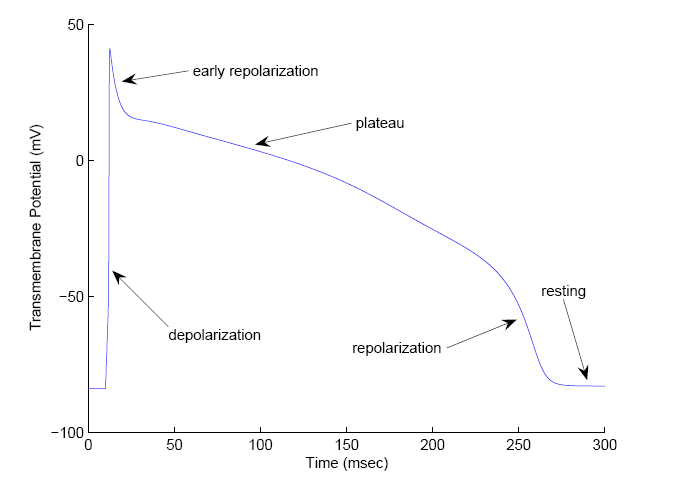
\includegraphics[width=0.8\textwidth,height=0.5\textwidth]{figures/LUO.png}
	\hspace{0.04\textwidth}
	\caption{Luo-Rudy I~模型的心肌细胞动作电位示意图\cite{Ying2005}}
	\label{f1} 
\end{figure}

去极化过程中,钠离子通道起关键作用,此时钠离子内流,导致细胞膜电位的上升,由-90mV上升至+30mV左右。这时心肌细胞的去极化程度达到最强,钠通道渐渐失活关闭,细胞开始进入复极化的状态。

复极化过程1期,即快速复极化初期,钠离子通道的渐渐关闭和钾离子外流的综合作用下,导致细胞膜电位由+30mV快速下降至0mV左右,所需时间大约10ms。复极化过程2期又称为缓慢复极期,当动作电位达到0mV左右之后,动作电位大概在0mV左右经历一段较长的持续时间,大约是100-150ms的平台期。这个阶段主要是钾离子外流和钙离子内流相互作用形成的。复极化过程3期,又叫做快速复极末期,这个阶段心肌细胞复极化加快,表现为钙离子内流减弱,钾离子外流加强,动作电位从0mV以比较快的速度下降到-90mV,持续时间大概100-150ms。至此,复极化过程完成,进入动作电位4 期,称为静息期。该时期细胞膜电位恢复到最初的静息电位状态。

(2)双域模型

在上世纪50年代,Hodgkin和Huxley通过对枪乌贼神经纤维细胞膜上离子电流的流动和电信号传导的研究,为细胞膜上的电生理学行为给出了定量的模型。将起到关键作用的离子通道抽象成是电阻可变的电路,钠离子,钾离子等跨膜流动形成的离子电流与跨膜电压,时间,电导和电容等物理量建立起数学关系,推导出经典的H-H方程
\cite{HH1952yu,HH1952,HH1952a,HH1952b},为以后基于心肌细胞电生理学模型的发展奠定了基础。FitzHugh\cite{FitzHugh1961}和Nagumo\cite{Nagumo1962}等人对H-H模型进行了简化和改进,提出了包含跨膜电势和单一恢复变量的双变量FitzHugh-Nagumo(FHN)模型。为了更贴近实验数据和心脏细胞结构的真实情况,电生理模型中涉及的膜模型也变得越来越复杂。Beeler和Reuter等人\cite{Beer1977}提出的模型涉及4种离子流,Luo和Rudy\cite{Luo1991}的模型中包含6种离子流,O'Hara等人\cite{ORD2011}基于非疾病人类心室实验数据提出的模型中有14种离子电流。这些模型在更好的反应心脏电生理学的运作机制的同时,涉及变量越来越多,并且可以运用到单细胞水平以及二维或者三维心脏组织结构上进行模拟\cite{3D1,3D2,3D3},相应带来的计算量也比较大。

随着进一步的研究,目前关于心肌细胞电势传播的仿真模拟模型发展为双域模型和单域模型两大方向。和单细胞模型中最明显的差异是这两种模型中都加入了扩散项,是偏微分方程和一系列常微分方程的耦合系统。最符合实际标准的心脏电活动的模拟需要考虑心脏结构中的纤维方向,电传导率的各向异性,心肌材料的不均匀性以及心肌细胞膜的特性等因素,双域模型\cite{bodo1983,EJ1,JS1} 被认为是最完整的描述心脏电活动的模型,更多的运用到心脏器官水平。心脏组织中细胞通过缝隙连接成为一个“整体”,双域模型假设心脏组织可以分为细胞内和细胞外两类区域,如图\ref{figbd}所示。
\begin{figure}[ht]
	\centering
	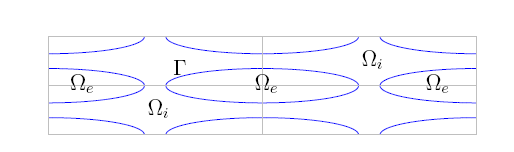
\includegraphics[width=0.65\textwidth,height=0.2\textwidth]{figures/ying.png}
	\hspace{0.04\textwidth}
	\caption{Intracellular and extracellular spaces $\Omega_i$ and $\Omega_e$ (4 rectangular cells) rated by the membrane $\Gamma$\cite{Ying2005}}
	\label{figbd} 
\end{figure}

双域模型的建立基于电势分布以及电荷和电流的守恒。通过广义欧姆定律来描述每个区域的动作电位,定义了从电势~$\phi(V)$,电流密度~$J$~和电导率张量~$D$~导出的电场~$E$~之间的关系。
\begin{equation}
E=-\nabla\phi,\quad J=DE=-D\nabla\phi.
\label{aa}
\end{equation}
考虑细胞内和细胞外空间:
\begin{equation}
J_i=-D_i\nabla\phi_i,\quad J_e=-D_e\nabla\phi_e,
\label{bb}
\end{equation}
其中,$J_i$~和~$J_e$~分别是细胞内和细胞外电流密度,$D_i$~和~$D_e$~分别是细胞内和细胞外电导率张量,$\phi_i$~和~$\phi_e$~是细胞内和细胞外的电势。
\begin{equation}
\nabla\cdot J_i=-I_m,\quad \nabla\cdot J_e=I_m, \quad\nabla(J_i+J_e)=0,
\label{cc}
\end{equation}
其中~$I_m$~是单位体积跨膜电流,它包含总的离子流~$I_{ion}$。
\begin{equation}
I_m=\beta_m\left(C_m\frac{\partial V_m}{\partial t}+I_{ion}+I_{app}\right),
\label{dd}
\end{equation}
其中~$\beta_m$~是心肌细胞的表面积-体积比,$C_m$~是指定的细胞膜电容,$I_{app}$~是刺激电流,$V_m$~是由下式给出的跨膜电压:
\begin{equation}
V_m=\phi_i-\phi_e.
\label{ee}
\end{equation}
由方程~(\ref{bb})和方程~(\ref{ee})可得:
\begin{equation}
\nabla\cdot D_i(\nabla V_m+\nabla\phi_e)=\beta_m\left(C_m\frac{\partial V_m}{\partial t}+I_{ion}+I_{app}\right),
\label{ff}
\end{equation}
\begin{equation}
\nabla\cdot\Big((D_i+D_e)\nabla\phi_e\Big)=-\nabla\cdot(D_i\nabla V_m).
\label{gg}
\end{equation}
(3)简化的单域模型

单域模型\cite{Cla2011,Per1993}是对双域模型的简化,相对双域模型计算量较少,更易于分析\cite{JS1}。 假设细胞内和细胞外空间的各向异性是相同的,即细胞外空间中的电导率与细胞内电导率成正比,$D_e=\lambda D_i$,其中~$\lambda$~是标量,表示细胞内和细胞外空间的电导率之间的比率。$\lambda$~值的选择可以决定生理意义上研究的准确性,但是选择一个能得到最好结果的值并不容易。使用单域模型的计算成本大约是使用双域模型的成本的十分之一到一半,这取决于所使用的细胞膜模型的复杂性。将~$D_e=\lambda D_i$~代入到方程~(\ref{gg}):
\begin{equation}
\nabla\cdot\Big((D_i+\lambda D_i)\nabla\phi_e\Big)=-\nabla\cdot(D_i\nabla V_m)
\label{h}
\end{equation}
\begin{equation}
\nabla\cdot(D_i\nabla\phi_e)=-\frac{1}{1+\lambda}\nabla\cdot(D_i\nabla V_m)
\label{i}
\end{equation}
将方程~(\ref{i})代入方程~(\ref{ff}):
\begin{equation}
\nabla\cdot\left(\frac{\lambda}{1+\lambda}D_i\nabla V_m\right)=\beta_m\left(C_m\frac{\partial V_m}{\partial t}+I_{ion}+I_{app}\right)
\label{j}
\end{equation}
如果我们引入有效电导率~$D=\frac{\lambda}{1+\lambda}D_i$\cite{ND1},我们获得了心脏组织的单域模型:
\begin{equation}
\nabla\cdot(D\nabla V_m)=\beta_m\left(C_m\frac{\partial V_m}{\partial t}+I_{ion}+I_{app}\right)
\label{k}
\end{equation}
\begin{equation}
\frac{\partial V_m}{\partial t}=-\frac{1}{C_m}(I_{ion}+I_{app})+(\frac{1}{C_m\beta_m})\nabla\cdot(D\nabla V_m)
\label{l}
\end{equation}
FitzHugh-Nagumo(FHN)单域模型指的是单域模型中的~$I_{ion}$~采用FitzHugh和Nagumo等人提出的膜模型,假设静息状态时的电势V为零,离子电流只使用一个恢复变量,即:
\begin{equation}
I_{ion}=cu(u-\alpha)(u-1)+w
\label{m}
\end{equation}
\begin{equation}
\frac{\partial w}{\partial t}=\varepsilon(u-\gamma w)
\label{n}
\end{equation}
$w$~是恢复变量,$u$~是标准的跨膜电势,定义为
\begin{equation}
u=\frac{V_m-V_{rest}}{V_p-V_{rest}}
\label{29}
\end{equation}
%$V_m$~是跨膜电势,$V_{rest}$~是静息电位,$V_p$~是高原电位\cite{Vig2008},$V_{th}$~是阈值电位,标准化的阈值电位~$\alpha$~也类似定义:
\begin{equation}
\alpha=\frac{V_{th}-V_{rest}}{V_p-V_{rest}}
\label{o}
\end{equation}
而O’Hara-Rudy dynamic(ORd)单域模型中的膜模型是2011年基于非病态的人类心室肌细胞的实验数据发展而来的\cite{ORD2011},属于离子通道模型,包含多种离子流:$I_{ion}=I_{Na}+I_{to}+I_{CaL}+I_{CaNa}+I_{CaK}+I_{Kr}+I_{Ks}+I_{K1}+I_{NaCa}+I_{NaK}+I_{Nab}+I_{Cab}+I_{Kb}+I_{pCa}$,并且涉及多个常微分方程,能更全面的反映心脏动作电位的特性。
\section{FHN、ORd单域模型研究现状}
心脏电势的传导机制对人体至关重要,对心脏电生理学的研究已经广泛存在。心脏电生理模型是一个非线性的反应-扩散系统,经研究表明,当心脏出现心律失常等疾病时,往往伴随着电势传播出现螺旋波的状态,心肌组织作为一种可激发系统,当系统不再处于平衡态的时候,螺旋波斑图会自发形成。
螺旋波的自组织和室速或者室颤的产生有一定的关系\cite{sprial2006},产生室速时,伴随着电折返形成螺旋波的状态,产生室颤时,则表现为螺旋波的破碎。可见螺旋波的稳定和失稳,对心率失常的影响很关键。双域模型由两个偏微分方程(PDE)和一系列描述细胞膜动力学的常微分方程(ODE)共同组成,双域方程求解对时间、空间离散化的要求比较高, 特别是在三维空间上求解数值解的计算量很大\cite{Clayton2008},直接求解双域模型仿真心脏各向异性兴奋传导的工作较难实现。单域模型作为简化的双域模型,除常微分方程外,只涉及一个偏微分方程,特别是FHN单域模型,只有两个变量,能够反映心脏电势传导的基本特性,已经有了大量的研究。

在非线性动力系统研究领域,对心脏电势传播中螺旋波的产生与消除的研究已经是一个趋势\cite{ouyang2001,yuan2005,tangguoning2010,gao2011}。 其中袁国勇等人在2005年研究了两个延迟耦合的FHN系统的动力学行为,分析了耦合强度范围,对一些螺旋波图形做了说明,2011年高加振等人采用了相空间压缩法,研究得出二维空间FHN系统中螺旋波的控制可以分为三个阶段。分数阶偏微分方程在生物,物理等领域也有一定的研究前景,一些专家学者,运用分数阶导数具有记忆和遗传的性质,来研究分数阶FHN方程\cite{LFW2012,Buweiping2015,LFW2015,YZZ2017}。 其中2012年Liu等人用隐式有限差分法求解了分数阶FHN单域模型,并给出了该方法的稳定性和收敛性。2017年Yang等人在不规则的二维区域上,用隐式向后欧拉有限元方法求解了分数阶FHN单域模型,展现了稳定的螺旋波图形。关于整数阶FHN单域模型也有许多数值方法,包括有限差分法,有限元方法,有限体积法等,Pertsov等人\cite{Pertsov1993}用有限差分法求解了FHN单域模型,研究了折返性势性心动过速的机制,Cherry 等人\cite{chafen2000}基于有限差分方法,提出了显式空间-时间自适应网格细化算法(AMRA),缩短了计算时间。Shuaiby 等人\cite{SM1} 运用了伽辽金有限元方法和算子分裂技术求解了FHN单域模型,显示激励扩散和复极化阶段的行为。Gerardo-Giorda\cite{GG2008}用半隐式有限元方法模拟激发前沿在心房细胞的传播,分别求解了FHN单域和双域方程,可以看出单域模型求解所用CPU 时间明显短于双域模型。Vincent 等人\cite{Vincent2015}提出高阶有限元方法,研究了通过使用高阶多项式有限元方法来减少自由度(DOF)数量的可能性,目标是显着提高分段线性有限元方法的仿真效率。Dickopf等人\cite{Dickopf2014}提出一种轻量级并行自适应方案设计与分析,提高了求解效率。Trangenstein等人\cite{Trangenstein2000}发展了算子分裂和有限元网格细化方法。已知心脏电生理波的模拟需要非常精细的网格,限制了当前数值模型对简化的几何形状和离子模型的适用性。在Belhamadia等人\cite{Belhamadia2009}的工作中,提出了一种基于时间依赖的各向异性网格重建的精确数值方法来模拟三维心脏电生理波。提出的数值方法大大减少了元素的数量,提高了电波前沿预测的准确性。Bendahmane等人\cite{Bendahmane2010}用有限体积法求解了FHN单域模型,并证明了该方法收敛于单域模型的弱解。Zhang等人\cite{zhang2005}用无网格有限元方法求解了FHN系统,研究了复杂的心脏几何形状,不均匀的纤维取向和不均匀的材料对电势传播的影响。Jackson\cite{Jackson1990,Jackson1992}证明了FHN单域模型精确解的存在性和唯一性,Jerome等人\cite{Jerome1980}和Sanfelici\cite{SAN1996}都利用有限元方法对反应-扩散系统进行了半离散空间近似的理论分析。

ORd单细胞模型是2011年基于人类心室肌细胞实验数据开发而来的,相对FHN模型的发展历程,时间较短。该模型涉及多个离子流及离子通道,能更好的反映心脏电活动的生理状态,由于心肌细胞动作电位的产生和离子通道的激活和失活状态密切相关,可以运用该模型来研究离子流的改变对心脏疾病的影响。Elshrif\cite{ovvr2015} 等人基于ORd单细胞模型,用Rush-Larsen(RL)方法求解了该模型,来研究心力衰竭状态下,跨膜动作电位的状态。Christophe\cite{ovvr2013} 等人通过改变ORd单细胞模型中~$I_{Na}$~等离子流的变化进行早期复极化(EAD)模拟,来研究影响早期复极化状态的因素,为某种室性心动过速疾病提供支持。
Chen等人\cite{ord1}用时间自适应方法结合RL等方法求解了ORd单细胞模型,使得动作电位的传播规律更精确。Whittaker等人\cite{ovvr2017}对ORd单域模型进行改进,用显式有限差分法研究了~$I_{Kr}$~等离子流通道的阻滞改变对短QT综合征(SQTS)的影响。
Trenor等人\cite{ovvr2012}分别在细胞和组织水平求解了ORd模型,研究离子通道阻滞对心律失常状态的影响,这些结果都为药物治疗提供了理论依据。
Elshrif等人\cite{ovvr20141}对ORd模型进行修改,开发了基于细胞水平的HF(心脏衰竭)模型,用了显式欧拉方法和RH方法,重现了心脏衰竭状态下人类心肌细胞的动作电位传播性质。Elshrif等人\cite{ovvr20142}又用同样的数值方法求解了二维ORd单域模型,研究了再重入波螺旋波的动力学行为,并与其它描述心脏肌细胞动作电位的模型进行了比较。Dutta等人\cite{ovvr20172}基于ORd模型,分别在单细胞和组织水平,模拟了急性心肌缺血状态下的动作电位复极化,传导速度等性质,并且在求解ORd单域模型中用了有限元方法。

心脏电活动的数值模拟,最开始是基于细胞水平的电生理模拟,将单个细胞兴奋的传播融入到心脏结构来进行电活动数值仿真。组织水平的研究通常看做是细胞间的耦合,一般是加入扩散项,常见的是在二维区域进行研究,如Bourgault\cite{2d2003}等人提出了基于非结构网格运用有限元方法求解了各向异性双域模型,展示螺旋波尖端更精细的动力学行为。随着人们对心脏结构及电生理机制产生越来越全面的认识,计算机水平的不断提高,基于整个心脏或者心室结构的电活动研究也受到广泛关注。首先需要得到心脏或者心室的三维结构,医学上可以通过CT(计算机断层扫描),MRI(核磁共振)等手段,这种方式需要考虑人的实体及一些副作用,不适合大范围研究使用。目前有许多方法构建三维的心脏或心室结构。Arevalo\cite{3d2007}等人使用基于解剖学的兔心室3D几何对双域模型进行了有限元方法数值模拟,心室表面和体积分别表示为非结构化三角形和四面体网格,对心律失常和心室颤动的机制有了更深的理解。Deuflhard\cite{3d2009}等人使用人类Auckland心脏3D几何形状,运用有限元空间和时间自适应方法求解了Aliev-Panfilov单域模型,获得的结果清楚地证明了在激发和平台阶段(正常传导)以及在重入激发(传导异常)之后心脏中电位的传播状态。Rodriguez\cite{3d2005}等人通过基于解剖学的兔子心脏,用半隐式可变步长有限元方法进行Beeler–Reuter双域模型求解,研究了左右心室腔几何形状的差异对电击的心脏易损性的影响。Prassl\cite{3d20009}等人提出了基于图像的非结构化网格生成技术,并用有限元方法求解了三维双域和单域模型。


\section{本文的研究内容}

心脏组织的电生理学模型正在应用于基础学科的研究,包括心律失常疾病,除颤研究等,借助计算机模拟心脏电势传导机制的模型,已经越来越普遍。本文主要用有限元方法求解了FHN单域模型,基于非线性反应项,采用显-隐时间离散的数值格式,证明了该完全离散的显-隐有限元方法的稳定性和收敛性,用二维数值算例验证了该方法的正确性,得到了稳定的螺旋波轨迹,验证了数值格式的时间和空间收敛阶符合理论证明,并将该方法拓展到三维人类左心室结构的计算中。本文中用了算子分裂技术将非线性反应-扩散偏微分方程分为线性偏微分方程和非线性常微分方程两部分。首先用有限元方法结合算子分裂技术求解了二维FHN单域模型,通过恰当的初边值条件,得到了稳定的螺旋波传播状态,并将该方法扩展到三维左右心室结构的数值模拟中。再用算子分裂有限元方法研究了基于三维左右心室结构的ORd单域模型,获得了跨膜电势的传播轨迹,可以为后续研究离子流的改变对心律失常等心脏疾病的影响奠定基础。本文各章节的组织结构如下:

第一章为绪论,主要介绍了心脏电生理模拟的研究背景及意义,目前描述组织及器官水平心脏电势传导机制的两大模型:双域模型和单域模型,以及FHN单域模型和ORd单域模型数值方法的研究现状。

第二章为有限元方法的基本思想,基本步骤,及有限元方法的数学基础,主要是泛函空间及相关不等式。

第三章介绍求解FHN单域模型的显-隐有限元方法,证明了二维情况下该数值格式的稳定性和收敛性,给定适当的初边值条件,得到了稳定的螺旋波运动轨迹,并将该方法应用到三维人类左心室结构的FHN单域模型求解中。

第四章介绍求解FHN单域模型的算子分裂有限元方法,在二维反应-扩散系统中,给定适当的初边值条件,也可以得到稳定的螺旋波状态,体现了算子分裂方法的正确性。基于三维左右心室结构,用该方法求解了FHN单域模型。

第五章介绍求解三维ORd单域模型的算子分裂有限元方法,得到了三维左右心室结构下跨膜电势的传播轨迹,可以为将来改变离子流来研究跨膜电势在病态情况下的传播规律提供支持。

第六章是对本文主体内容的总结,对以后的工作进展进行了概括。



\chapter{有限元方法}
%==============第二章节内容==================
航空航天工程,机械工程,生物力学\cite{FEM2010}等工程领域中常常涉及一些物理问题,比如弹性力学,电磁场,热传导等问题,这些问题大多可以用偏微分方程来描述。通常根据实际问题,其方程及其边界条件,几何形状等比较复杂的情况下,很难得到方程的解析解,这时候就需要运用数值离散方法得到近似解。有限元方法就是一种常用且高效的数值计算方法,在流体力学,结构力学等方面应用十分广泛\cite{begin1986}。早在19世纪40年代就有了有限元的基本思想\cite{Courant1943},1956年Turner等人\cite{Turner1956} 发表了在结构力学中运用有限元思想的文章,对飞机结构进行“单元”划分,并对形成的刚度矩阵进行了分析。1960年Clough等人\cite{Clough1960}在用有限元思想进行平面应力分析的文章中,第一次明确提出“有限元方法”(finite element method)的术语。在国内,胡海昌\cite{Hu1954} 在1954年提出了广义变分原理,为研究近似数值解提供了理论依据,冯康是我国有限元方法的创始人,1965年他的著作\cite{Feng1965}《基于变分原理的差分格式》,标志着有限元方法在中国的诞生,为计算数学的发展产生了深远影响。19世纪80年代以来,石钟慈对非协调有限元的收敛性证明方面做出了贡献\cite{shi2000},90年代以来,间断有限元的发展在实际工程问题中也发挥越来越大的作用\cite{Feng2001}。随着有限元分析软件渐渐成熟\cite{ANSYS2000},使得有限元方法的应用前景更广阔。
\section{有限元方法的基本思想}
有限元法的基本思想是将微分方程连续的计算区域进行离散,剖分成有限个单元,这些单元通过节点按一定的方式相互连接但是互不重叠。在每个单元内选取恰当节点和插值基函数,近似解可以由节点值和单元基函数的线性组合来表示。这里运用分片插值的思想,其作为有限元方法的核心,是与里兹法(Ritz)的重要区别。在有限元方法的实现过程中,单元剖分类型,插值基函数的选取等对近似解收敛于解析解十分重要,误差估计和网格自适应技术也是研究的方向。

有限元方法的变分原理是基于待求解方程及其边界条件的等价积分形式,使得有限元方法有严谨的理论基础支撑。有限元方法的通用性较高,对不规则的空间几何现状,复杂的边界条件,不同材料特性,非线性问题等都能有效处理,有很好的适应性。除此之外,有限元方法求解过程中会转化为矩阵代数问题,通过计算机编程,运用并行化等新技术,可支持高效率的数值计算。在流体力学,电磁力学,以及不同物理场的耦合问题有广泛的应用。
\section{有限元方法的基本步骤}
(1)单元划分
根据求解区域的形状,选择符合要求的单元几何形状,将求解区域剖分成互不重叠的有限单元,即剖分逼近,化繁为简。单元形状不会限制规则划分,是和有限差分法相比的一大优势。单元剖分一般要求简单化,便于建立相关方程;尽量精确,所有剖分单元与原始求解区域相同;单元剖分数量根据实际问题灵活选取,以免造成太大计算量。常见的二维区域上的剖分形状有三角形,四边形等。三维区域上有四面体,六面体单元等。

(2)单元分析
对剖分得到的单元,选择合适的节点与插值基函数,将待求解函数表示为节点及其插值基函数之间的关系,通过物理状态或者数学分析,可以构建单元节点上的待求解函数值和外界条件之间的方程组,称之为单元方程组。一般常用多项式作为插值基函数,方便进行积分等操作。单元刚度矩阵和单元方程组的推导一般有直接平衡法,功和能量法,加权残余法\cite{L2003}。

(3)系统综合
根据有限个单元之间的关系,可以利用单元方程组得到整个求解区域上的总体方程组。

(4)初边值条件
根据待求解问题中已知的初边值条件,修改总体方程组。

(5)方程组求解
修改后的总体方程组一般是代数方程组,可以运用消元法,迭代法等数值方法进行求解,得到待求解函数的近似解。
\section{有限元方法的数学基础}
\newtheorem{Definition}{\hspace{2em}定义}[chapter]
\begin{Definition}
[范数\cite{fanhan2006}]{
	线性空间$X$上的范数$\| \cdot\|$是一个非负函数:$X\rightarrow R^1$满足:
	
	$(1) \|x\|\geq0$   \quad$($正定性$)$;
	
	$(2) \|x+y\|\leq\| x\|+\| y\| \quad (\forall x,y\in X)$  \quad$($三角不等式$)$;
	
	$(3) \| \alpha x\|=\mid \alpha\mid\| x\| \quad(\forall\alpha\in K,\forall x\in X)$  \quad$($齐次性$)$.
}
\end{Definition}
\begin{Definition}
	[$L^p(\Omega)(1\leq p<\infty)$空间]{
	$\Omega$是$R^n$中的可测集,将在$\Omega$上可测,并且$\mid u(x)\mid$在$\Omega$上可积的函数$u(x)$的全体构成的空间记为$L^p(\Omega)$。其范数定义为
	\begin{equation*}
	\| u\|_{L^p(\Omega)}=(\int_\Omega\mid u(x)\mid^pdx)^{\frac{1}{p}},
	\end{equation*}
	其中$L^2(\Omega)$内积规定为
	\begin{equation*}
	(u,v)=\int_\Omega uvdx.
	\end{equation*}}
\end{Definition}

\begin{Definition}
[$L^\infty(\Omega)$空间]{
	$\Omega$是$R^n$中的可测集,将在$\Omega$上本性有界可测函数$u(x)$的全体构成的空间记为$L^\infty(\Omega)$。其范数定义为
	\begin{equation*}
	\| u\|_{L^\infty}=ess\sup_{x\in\Omega}\mid u(x)\mid.
	\end{equation*}}
\end{Definition}
\begin{Definition}
[$H\ddot{o}lder$不等式]{
	设$p>1$,$\frac{1}{p}+\frac{1}{q}=1$,若$f(x)\in L^p(\Omega)$,$g(x)\in L^q(\Omega)$,则$f(x)g(x)\in L^1(\Omega)$,且
	\begin{equation*}
	\int_\Omega\mid f(x)g(x)\mid dx\leq(\int_\Omega\mid f(x)\mid^p)^{\frac{1}{p}}(\int_\Omega\mid g(x)\mid^q)^{\frac{1}{q}},
	\end{equation*}
	即$\| fg\|_{L^1(\Omega)}\leq\| f\|_{L^p(\Omega)}\| g\|_{L^q(\Omega)}$。当且仅当$\mid f(x)\mid=C\mid g(x)\mid^{\frac{q}{p}}$ 或$\mid g(x)\mid=C\mid f(x)\mid^{\frac{p}{q}}$时等号成立。
}
\end{Definition}
\begin{Definition}
[$H\ddot{o}lder$不等式的推广\cite{holder2013}]
{
	设$\lambda_1+\lambda_2+...+\lambda_k=1$,$\lambda_j>0$,且对于函数$f_j(j=1,2,3...,k)$, $\int_\Omega\mid f_j(x)\mid^{\frac{1}{\lambda_j}}<\infty$ 成立,则函数$f_1f_2...f_k$是Lebesgue可积的,且有下列不等式成立
	\begin{equation*}
	\int_\Omega\mid f_1f_2...f_k\mid dx\leq(\int_\Omega\mid f_1\mid^{\frac{1}{\lambda_1}})^{\lambda_1}(\int_\Omega\mid f_2\mid^{\frac{1}{\lambda_2}})^{\lambda_2}...(\int_\Omega\mid f_k\mid^{\frac{1}{\lambda_k}})^{\lambda_k}.
	\end{equation*}
}
\end{Definition}
\begin{Definition}
   [Minkowski不等式]
   {
   	设$p\geq1$,若$f(x)$,$g(x)\in L^p(\Omega)$,则$f(x)+g(x)\in L^p(\Omega)$,且
   	\begin{equation*}
   	\| f+g\|_p\leq\| f\|_p+\| g\|_p,
   	\end{equation*}
   	当且仅当$\exists k_1$,$k_2\geq0$,$k_1+k_2>0$ ,使$k_1f(x)=k_2g(x)$ 成立时等号成立。
   }
\end{Definition}

\begin{Definition}
	[Cauchy-Schwarz不等式]{
		设$(X,(\cdot,\cdot))$是内积空间,令$\| x\|=(x,x)^{\frac{1}{2}}\quad(\forall x\in X)$,则
		\begin{equation*}
		\mid (x,y)\mid\leq\| x\|\| y\| \quad(\forall x,y\in X),
		\end{equation*}
		当且仅当$x$与$y$线性相关时等号成立。
	}
\end{Definition}

$\Omega$是$n$维空间$R^n$中的开子集,$C^\infty_0(\Omega)$表示在$\Omega$上无穷次可微函数的集合,并且这些函数的紧支集也在$\Omega$内。多重指标$\alpha=(\alpha_1,\alpha_2,...,\alpha_n)\in N^n$,记$\mid \alpha\mid=\alpha_1+\alpha_2+...+\alpha_n$。偏导数算子有如下形式
\begin{equation*}
\partial^\alpha=\frac{\partial^{\mid \alpha\mid}}{\partial^{\alpha_1}_{x_1}...\partial^{\alpha_n}_{x_n}}.
\end{equation*}
\begin{Definition}
[广义导数\cite{Shi2010}]{
	假设$u$在$\Omega$上是局部Lebesgue可积函数,如果存在$\Omega$上的局部Lebesgue可积函数$v$,满足以下等式
	\begin{equation*}
	\int_\Omega v\varphi dx=(-1)^{\mid \alpha\mid}\int_\Omega u\partial^\alpha\varphi dx  \quad \forall\varphi\in C^\infty_0(\Omega),
	\end{equation*}
	称$v$是$u$的一个广义导数,记为$\partial^\alpha u$。}
\end{Definition}
\begin{Definition}
	[Sobolev 空间\cite{Chen2010}]{
		$W^{k,p}(\Omega)=\{u\in L^p(\Omega):\partial^\alpha u\in L^p(\Omega) \mid \alpha\mid\leq k\}$,其中~$k$为非负整数,$p\geq1$。有以下范数定义
		\begin{equation*}
		\| u\|_{W^{k,p}(\Omega)}=\left\{\begin{aligned}&(\sum_{\mid \alpha\mid\leq k}\| \partial^\alpha u\|^p_{L^p(\Omega)})^{1/p},\quad 1\leq p<+\infty;\\&\max_{\mid \alpha\mid\leq k}\| \partial^\alpha u\|_{L^\infty(\Omega)},\quad p=+\infty.\end{aligned}\right.
		\end{equation*}
		称赋范线性空间~$W^{k,p}(\Omega)$为Sobolve空间。当~$p=2$时,还可以定义
		\begin{equation*}
		H^k(\Omega)=W^{k,2}(\Omega),\quad H^k_0(\Omega)=W^{k,2}_0(\Omega).
		\end{equation*}
		引入內积
		\begin{equation*}
		(u,v)_{k,\Omega}=\sum_{\mid \alpha\mid\leq k}\int_\Omega\partial^\alpha u\partial^\alpha vdx,
		\end{equation*}
		当$k=0$时,$W^{0,p}(\Omega)=L^p(\Omega)$.}
\end{Definition}
\begin{Definition}
	[嵌入定理\cite{qianru2012}]{
		设$m$为非负整数,$m\geq1$, $1\leq p\leq\infty$,$\Omega\subset R^n$的开子集,并且边界满足Lipschitz连续,则有如下嵌入关系成立:
		\begin{equation*}
		W^{m,p}\hookrightarrow\left\{\begin{aligned}&L^{q}(\Omega), \frac{1}{q}=\frac{1}{p}-\frac{m}{n}>0,
		\\&L^q_{loc}(\Omega),\forall q,1\leq q\leq\infty, \frac{1}{q}=\frac{m}{n}.\end{aligned}\right.
		\end{equation*}
	}
\end{Definition}
\begin{Definition}
[紧嵌入定理]{
	若$\Omega$有界,有下列紧嵌入关系成立:
	\begin{equation*}
	W^{m,p}\hookrightarrow\left\{\begin{aligned}&L^{q}(\Omega), \forall1\leq q<p^*, \frac{1}{p^*}=\frac{1}{p}-\frac{m}{n}, m<\frac{n}{p},
	\\&L^q(\Omega),\forall q\in[1,\infty), m=\frac{n}{p}.\end{aligned}\right.
	\end{equation*}
	最常用的情况为
	\begin{equation*}
	n=2, H^1(\Omega)\hookrightarrow L^q(\Omega), \forall 1\leq q\leq\infty.
	\end{equation*}
}
\end{Definition}




\section{本章小结}
本章主要介绍了有限元方法的起源与发展,阐述了有限元方法的基本思想和基本步骤,对本文有限元理论中涉及到的泛函空间及不等式做了说明,为完全离散显-隐有限元方法的稳定性和收敛性分析提供理论基础。

%==============第三章节内容==================
\chapter{FHN单域模型的显-隐有限元方法}

反应-扩散模型已经在化学,物理学,工程学和生物学中有许多应用\cite{ouyang2000}。心脏中心律不齐等疾病的产生可能与心脏电势传播形成螺旋波的现象密切相关。螺旋波的产生机制就属于反应-扩散系统范畴,并且可以作为可激发系统,在双域或者单域模型中表现为动作电位的扩布过程。计算心脏学中,这种反应-扩散系统是由一系列非线性微分方程耦合形成的。
FHN单域模型是描述心脏电势传播规律的FHN双域模型的简化,由一个偏微分方程和常微分方程耦合组成的反应-扩散系统,如下形式\cite{Belhamadia2009}。
\begin{equation}
\left\{\begin{aligned}&\frac{\partial u}{\partial t}=\nabla\cdot(\textbf{K}\nabla u)+I_{ion}(u,v)+I_s,\\&\frac{\partial v}{\partial t}=F(u,v).\end{aligned}\right.
\label{system}
\end{equation}
这是一个无量纲的双变量系统,其中~$u$~是跨膜电势,$v$~是恢复变量,$\textbf{K}$~是扩散系数,$I_s$代表外部刺激项,$I_{ion}$~代表跨膜离子流。%gating 表征细胞膜对不同离子的渗透性
\section{时间离散}
因为单域模型中涉及一个抛物型方程,我们先考虑简单的抛物方程:
\begin{equation*}
\left\{\begin{aligned}&\frac{\partial u}{\partial t}=\nabla^{2}u+f(u) \quad\Omega\times(0,T],\\&u=u_D \quad\partial\Omega\times(0,T],\\&u=u_0\quad t=0.\end{aligned}\right.
\label{1.1}
\end{equation*}
假设$\Omega$是二维区域,我们用有限差分逼近来近似时间导数,时间离散可以有多种格式,常见的有显格式,隐格式,半隐(显-隐)格式,Crank–Nicolson格式。
首先用~$u^n$~表示~$u(n\Delta t)$,$\Delta t$表示时间步长,有以下时间离散格式:

(1) 显格式(向前欧拉)
\begin{equation}
\frac{u^{n+1}-u^n}{\Delta t}=\nabla^2u^{n}+f(u^{n}).
\end{equation}

(2) 隐格式(向后欧拉)
\begin{equation}
\frac{u^{n+1}-u^n}{\Delta t}=\nabla^2u^{n+1}+f(u^{n+1}).
\end{equation}

(3) 显-隐格式(半隐格式)
\begin{equation}
\frac{u^{n+1}-u^n}{\Delta t}=\nabla^2u^{n+1}+f(u^{n}).
\end{equation}

(4) Crank–Nicolson格式
\begin{equation}
\frac{u^{n+1}-u^n}{\Delta t}=\frac{1}{2}(\nabla^2u^{n+1}+\nabla^2u^{n})+f(u^{n}).
\end{equation}
总的来说,除去半隐格式,其余三种离散格式可以写成一个通用的~$\theta$~格式,即
\begin{equation}
\frac{u^{n+1}-u^n}{\Delta t}=\theta\nabla^2u^{n+1}+(1-\theta)\nabla^2u^{n}+f(u^{n}).
\end{equation}
当~$\theta=0$~时,对应向前欧拉格式,当~$\theta=1$~时,对应向后欧拉格式,当~$\theta=\frac{1}{2}$~时,对应Crank–Nicolson格式。
这几种方法比较常用,有各自的特点。完全显式的方法,不用求解代数方程组,编程简单,但是求解时,时间和空间步长需要满足一定的关系,才能保证数值格式的稳定性。完全隐式的方法,没有时间步长的限制,但需要在每个时间层求解代数方程组,特别计算大型非线性方程组时,需要更多的计算时间。显-隐格式是一个比较折中的方法,一般隐式的求解方程中的一些项(例如线性项),显式的求解方程中其余项(例如非线性项),对时间步长的要求不是很高,并且求解的是线性方程组。Crank–Nicolson~格式相对更精确,时间方向达到二阶精度。本节中时间离散采用的是显-隐格式。


\section{控制方程}
本文研究了二维和三维FHN单域模型,FHN单域模型的具体形式及满足的初边值条件为
\begin{equation}
\left\{\begin{aligned}&\frac{\partial u}{\partial t}=\nabla\cdot(\textbf{K}\nabla u)+G(u)u-v\quad (\textbf{x},t)\in\Omega\times(0,T],\\&\frac{\partial v}{\partial t}=\varepsilon(\beta u-\gamma v-\delta)\quad (\textbf{x},t)\in\Omega\times(0,T],\\&u(\textbf{x},0)=\psi(\textbf{x}),v(\textbf{x},0)=\varphi(\textbf{x})\quad \textbf{x}\in\Omega,
\\&u(\textbf{x},t)=0, v(\textbf{x},t)=0\quad (\textbf{x},t)\in\partial\Omega\times (0,T),
\end{aligned}\right.
\label{1}
\end{equation}
其中$\Omega$可以表示二维$(\textbf{x}=(x,y))$和三维$(\textbf{x}=(x,y,z))$有界区域,$I_{ion}(u,v)=G(u)u-v$,$G(u)u=(1-u)(u-a)u$,$0< a<1$,$I_s=0$,$F(u,v)=\varepsilon(\beta-\gamma v-\delta)$,$\varepsilon\beta>0$,$\varepsilon\gamma$,$\varepsilon\delta\geq0$。

本文中先用显-隐有限元方法求解二维FHN单域模型,并证明了完全离散的显-隐有限元方法数值格式的稳定性和收敛性,给出相应数值算例进行验证。
本文中符号$(\cdot,\cdot)$表示为$L^2(\Omega)$中的内积,$\|\cdot\|=\| \cdot\|_{L^2(\Omega)}$,$\|\cdot\|_k=\| \cdot\|_{H^k(\Omega)}$,$\|\cdot\|_{0,\mu}=(\int^T_0\| \cdot\|^2_\mu dt)^{\frac{1}{2}}$。
\section{二维FHN单域模型变分和离散形式}
\subsection{变分形式}
考虑系统~(\ref{1})的有限元变分形式,将整个方程系统两边同时乘以测试函数,并将偏微分方程中的扩散项进行分部积分,有~$u(t)$,$v(t)\in U$,使得
\begin{equation}
\left\{\begin{aligned}&(u_t,p)+a(u,p)=\big(G(u)u,p\big)-(v,p)\quad \forall p\in V,t\in(0,T],\\&(v_t,q)=\big(\varepsilon(\beta u-\gamma v-\delta),q\big)\quad \forall q\in V,t\in(0,T],\\&\big(u(x,y,0),p\big)=(u_0,p),\big(v(x,y,0),q\big)=(v_0,q)\quad \forall p,q\in V,\end{aligned}\right.
\label{2}
\end{equation}
成立,其中~$U=L^2(0,T;V)$,$V=H^1_0(\Omega)$~是标准的Sobolev空间,$a(u,p)=\int_\Omega K\nabla u\cdot\nabla p dx$。关于连续问题~(\ref{2})中解的存在唯一性结果可参考\cite{exist1978,bianzhi1978}。
\subsection{完全离散的显-隐有限元方法}
我们假设~$\mathcal {T}_h$~是对有界区域~$\Omega$~的三角剖分,$h$~表示所有剖分单元的最大直径。针对变分形式~(\ref{2}),将无限维的空间~$V$~中的求解问题转化为离散(有限维)空间~$V_h$ 中的问题,$V_h\in V$,并称~$V_h$~为有限元空间,定义如下:
\begin{equation*}
V_h=\{p_h,q_h\in H_0^1(\Omega):p_h,q_h|_K\in P_s(K),\quad\forall K\in \mathcal {T}_h\},
\label{hs}
\end{equation*}
其中~$P_s(K)$~是多项式函数空间,其中最高次幂为~$s$。

记~$\tau=T/M$~为时间步长,$M$~为正整数。$u^n_h$,$v^n_h$~是精确解~$u(t)$~和~$v(t)$~在空间~$V_h$~中,$t=t_{n}=n\tau$, ($n=0,1,...,M-1$)时刻的近似。我们用
\begin{equation*}
\bar{\partial}_tu^{n+1}=\frac{u^{n+1}-u^n}{\tau},\quad\bar{\partial}_tv^{n+1}\\=\frac{v^{n+1}-v^n}{\tau}
\end{equation*}
来近似时间导数。偏微分方程中扩散项是隐格式,反应项作为非线性三次多项式,本文做了简单的线性化,而常微分方程则采用隐格式,最终完全离散的显-隐有限元方法就是对于~$n=0,1,...,M-1$~ 有~$u^{n+1}_h,v^{n+1}_h\in V_h$~并且对~$t\in (0,T]$,$p_h,q_h\in V_h$,使得
\begin{equation}
\left\{\begin{aligned}&(\bar{\partial}_tu^{n+1}_h,p_h)+a(u^{n+1}_h,p_h)=\big(G(u^n_h)u_h^{n+1},p_h\big)-(v_h^n,p_h)\quad p_h\in V_h,\\&(\bar{\partial}_tv^{n+1}_h,q_h)=\big(\varepsilon(\beta u^{n+1}_h-\gamma v^{n+1}_h-\delta),q_h\big)\quad \forall q_h\in V_h,t\in(0,T],\\&u^0_h=u_{h0},v^0_h=v_{h0}.\end{aligned}\right.
\label{4}
\end{equation}
成立,其中~$u_{h0},v_{h0}$~是初值~$u_0,v_0$~在~$V_h$~中的逼近。
在下一节,我们分析了完全离散的数值格式~(\ref{4})的稳定性,本文中~$C$~为与~$h$~无关的正常数。
\newpage
\subsection{稳定性分析}
\newtheorem{theorem}{\hspace{2em}定理}[chapter]
\newtheorem{lemma}{\hspace{2em}引理}[chapter]
\begin{lemma}[Gronwall's Lemma\cite{He2003}]
	令~$a_k$,$b_k$,$c_k$,$d_k$~$($整数$k\geq0$$)$和~$C_0$~为非负数,有
	\begin{equation*}
	a_n+\triangle t\sum^n_{k=0}b_k\leq\triangle t\sum^{n-1}_{k=0}d_ka_k+\Delta t\sum^{n-1}_{k=0}c_k+C_0   \quad \forall n\geq1,
	\label{5}
	\end{equation*}
	\begin{equation*}
	a_n+\triangle t\sum^n_{k=0}b_k\leq exp\left(\triangle t\sum^{n-1}_{k=0}d_k\right)\left( \triangle t\sum^{n-1}_{k=0}c_k+C_0\right)  \quad \forall n\geq1.
	\label{6}
	\end{equation*}
	\label{yinli1}
\end{lemma}
\begin{theorem}[稳定性]
	假设~$u^{n+1}_h$~和~$v^{n+1}_h$~是完全离散显-隐有限元方法数值格式~$(\ref{4})$的数值解。 如果~$\tau<\min\{\frac{2}{(1-a)^2+2+2\varepsilon^2\beta^2},\frac{1}{2(1-\varepsilon\gamma)}\}$,则
	\begin{equation*}
	\parallel u^{n+1}_h\parallel^2+\parallel v^{n+1}_h\parallel^2+\frac{2\tau\alpha}{A}\sum^n_{k=0}\parallel u^{k+1}_h\parallel^2_1\leq \frac{q_n}{A}\exp(\frac{B}{A}n),
	\end{equation*}
	\label{the:the1}
	其中$A=\min\{1-\tau\left(\frac{(1-a)^2+2}{2}+\varepsilon^2\beta^2\right),1-2\tau(1-\varepsilon\gamma)\}$,$B=\max\{\tau\left(\frac{(1-a)^2+2}{2}+\varepsilon^2\beta^2\right),\tau\\(3-2\varepsilon\gamma)\}$,$q_n=\parallel u^0_h\parallel^2+(1+\tau)\parallel v^0_h\parallel^2+\tau(n+1)(\varepsilon\delta)^2$。
	\label{the:the1}
\end{theorem}

证明:我们很容易得到系统~(\ref{2})中的双线性形式~$a(u,p)$~是有界并且强制的,存在常数~$\alpha$,$\beta>0$~使得
\begin{equation*}
\mid a(u,p)\mid\leq\beta\| u\|_1\| p\|_1, \quad a(p,p)\geq \alpha\| p\|^2_1,\quad\forall u,p\in H_0^1(\Omega).
\label{7}
\end{equation*}
令~$p_h=u^{n+1}_h$,$q_h=v^{n+1}_h$,可以得到
\begin{equation}
\left\{\begin{aligned}&(\bar{\partial}_tu^{n+1}_h,u^{n+1}_h)+a(u^{n+1}_h,u^{n+1}_h)=\big(G(u^n_h)u_h^{n+1},u^{n+1}_h\big)-(v_h^n,u^{n+1}_h), \\&(\bar{\partial}_tv^{n+1}_h,v^{n+1}_h)=\big(\varepsilon(\beta u^{n+1}_h-\gamma v^{n+1}_h-\delta),v^{n+1}_h\big).\end{aligned}\right.
\label{8}
\end{equation}
\begin{equation}
\begin{split}
(G(u^n_h)u_h^{n+1},u^{n+1}_h)&=\big((1+a)u^n_hu^{n+1}_h,u^{n+1}_h\big)-\big((u^n_h)^2u^{n+1}_h,u^{n+1}_h\big)-a(u^{n+1}_h,u^{n+1}_h)\\
&\leq(1+a)\| u^n_hu^{n+1}_h\|\| u^{n+1}_h\|-\| u^n_hu^{n+1}_h\|^2-a\| u^{n+1}_h\|^2\\
&\leq\frac{(1-a)^2}{4}\| u^{n+1}_h\|^2.
\end{split}
\label{9}
\end{equation}
通过~$2(x-y,x)\geq\mid x\mid^2-\mid y\mid^2$,(\ref{9})和Cauchy-Schwarz不等式,~(\ref{8})满足
\begin{equation*}
\begin{split}
&\| u^{n+1}_h\|^2-\| u^{n}_h\|^2+\| v^{n+1}_h\|^2-\| v^n_h\|^2+2\tau\alpha\| u^{n+1}_h\|^2_1 \\
&\leq\tau\Big(\frac{(1-a)^2+2}{2}-(\varepsilon\beta)^2\Big)\|u^{n+1}_h\|^2+\tau(2-2\varepsilon\gamma)\|v^{n+1}_h\|^2+\tau\|v^{n}_h\|^2+\tau (\varepsilon\delta)^2.
\end{split}
\label{10}
\end{equation*}
将上式从0到~$n$~进行累加,有
\begin{equation*}
\begin{split}
&\Big(1-\tau\frac{(1-a)^2+2}{2}-\tau\varepsilon^2\beta^2\Big)\| u^{n+1}_h\|^2+\big(1-2\tau(1-\varepsilon\gamma)\big)\| v^{n+1}_h\|^2+2\tau\alpha\sum^{n}_{k=0}\parallel u^{k+1}_h\parallel^2_1\\
&\leq\tau\left(\frac{(1-a)^2+2}{2}+\varepsilon^2\beta^2\right)\sum^n_{k=1}\parallel u^k_h\parallel^2+\tau(3-2\varepsilon\gamma)\sum^n_{k=1}\parallel v^k_h\parallel^2\\
&\quad+\parallel u^0_h\parallel^2+(1+\tau)\parallel v^0_h\parallel^2+\tau(n+1)(\varepsilon\delta)^2.
\end{split}
\label{12}
\end{equation*}
令~$A=\min\{1-\tau\left(\frac{(1-a)^2+2}{2}+\varepsilon^2\beta^2\right),1-2\tau(1-\varepsilon\gamma)\}$,
$B=\max\{\tau\left(\frac{(1-a)^2+2}{2}+\varepsilon^2\beta^2\right),\\\tau(3-2\varepsilon\gamma)\}$,$q_n=\parallel u^0_h\parallel^2+(1+\tau)\parallel v^0_h\parallel^2+\tau(n+1)(\varepsilon\delta)^2$,当 ~$\tau<\min\{\frac{2}{(1-a)^2+2+2\varepsilon^2\beta^2},\\\frac{1}{2(1-\varepsilon\gamma)}\}$。
运用引理~\ref{yinli1},有
\begin{equation*}
\parallel u^{n+1}_h\parallel^2+\parallel v^{n+1}_h\parallel^2+\frac{2\tau\alpha}{A}\sum^n_{k=0}\parallel u^{k+1}_h\parallel^2_1\leq \frac{1}{A}q_n\exp(\frac{B}{A}n).
\end{equation*}
至此完成了完全离散的显-隐有限元方法数值格式的稳定性证明。接下来证明该数值格式的收敛性之前,先证明数值解~$u_h^{n+1}$~在~$H^1$~范数意义下的有界性。
\begin{theorem}
	假设~$\tau<\min\{\frac{2}{(1-a)^2+2+2\varepsilon^2\beta^2},\frac{1}{2(1-\varepsilon\gamma)},\frac{1}{2\varepsilon^2\beta^2},\frac{2}{3-4\varepsilon\gamma}\}$,有以下不等式成立
	\begin{equation*}
	(1-2\tau\varepsilon^2\beta^2)\|u^{n+1}_h\|^2_{1}\leq C\|u^n_h\|^2_{1}+C.
	\label{13}
	\end{equation*}
	\label{thm2}
\end{theorem}

证明:令~$p_h=\frac{u^{n+1}_h-u^n_h}{\tau}$,$q_h=v^{n+1}_h$,系统~(\ref{4})可变为
\begin{equation*}
\left\{\begin{aligned}&(\bar{\partial}_tu^{n+1}_h,\bar{\partial}_tu^{n+1}_h)+a(u^{n+1}_h,\bar{\partial}_tu^{n+1}_h)
=\Big(G(u^n_h)u_h^{n+1},\bar{\partial}_tu^{n+1}_h\Big)-(v_h^n,\bar{\partial}_tu^{n+1}_h), \\&(\bar{\partial}_tv^{n+1}_h,v^{n+1}_h)=\Big(\varepsilon(\beta u^{n+1}_h-\gamma v^{n+1}_h-\delta),v^{n+1}_h\Big).\end{aligned}\right.
\label{14}
\end{equation*}
从定理~\ref{the:the1},我们可以得到下列不等式
\begin{equation}
\begin{split}
\Big(G(u^n_h)u_h^{n+1},~&\bar{\partial}_tu^{n+1}_h\Big)=\frac{1}{\tau}\Big(\big((1+a)u^n_h-a-(u^n_h)^2\big)u^{n+1}_h,u^{n+1}_h-u^n_h\Big)\\
&\leq\frac{1}{\tau}\Big(\frac{2a+3+3a^2}{4}\|u^{n+1}_h\|^2+\frac{3(1+a)^2}{4}\|u^{n}_h\|^2+a\|u^{n+1}_h\|\|u^n_h\|\\
&\quad+C\frac{q_n}{2\tau\alpha}\exp(\frac{B}{A}n)\|u^n_h\|^2_{1}\Big),
\label{15}
\end{split}
\end{equation}
其中~$A$,$B$~和~$q_n$是~$\tau$~满足一定条件时,定理~\ref{the:the1}中相对应的项。
\begin{equation}
a(u^{n+1}_h,\bar{\partial}_tu^{n+1}_h)\geq\frac{1}{2\tau}(\|u^{n+1}_h\|^2_{1}-\|u^n_h\|^2_{1}),
\label{16}
\end{equation}
\begin{equation}
(v^n_h,\bar{\partial}_tu^{n+1}_h)\leq\frac{1}{\tau}\|v^n_h\|(\|u^{n+1}_h\|+\|u^n_h\|),
\label{17}
\end{equation}
\begin{equation}
\|v^{n+1}_h\|^2-\|v^n_h\|^2\leq2\tau(\varepsilon\beta)^2\|u^{n+1}_h\|^2_{1}+\tau(\frac{3}{2}-2\varepsilon\gamma)\|v^{n+1}_h\|^2+\tau(\varepsilon\delta)^2.
\label{18}
\end{equation}
将~(\ref{15})-(\ref{18})相加,有
\begin{equation*}
\begin{split}
(1-&2\tau\varepsilon^2\beta^2)\|u^{n+1}_h\|^2_{1}+(1-\frac{3\tau}{2}+2\tau\varepsilon\gamma)\|v^{n+1}_h\|^2\leq2\Big(\frac{2a+3+3a^2}{4}\|u^{n+1}_h\|^2+C\|u^n_h\|^2_1\\
&+\frac{3(1+a)^2}{4}\| u^n_h\|^2+a\| u^{n+1}_h\|\| u^n_h\|\Big)+2\|v^n_h\|(\|u^{n+1}_h\|+\|u^n_h\|)+\|v^n_h\|^2+\tau \varepsilon^2\delta^2.
\label{19}
\end{split}
\end{equation*}
如果~$\tau<\min\{\frac{2}{(1-a)^2+2+2\varepsilon^2\beta^2},\frac{1}{2(1-\varepsilon\gamma)},\frac{1}{2\varepsilon^2\beta^2},\frac{2}{3-4\varepsilon\gamma}\}$,有
\begin{equation*}
\begin{split}
(1-2\tau\varepsilon^2\beta^2)\|u^{n+1}_h\|^2_{1}&\leq C\|u^n_h\|^2_{1}+C.
\label{20}
\end{split}
\end{equation*}
下一节证明完全离散的显-隐有限元方法的收敛性。
\subsection{收敛性分析}
首先我们介绍插值算子$I_h :H^{s+1}(\Omega)\rightarrow V_h$,满足以下不等式 \cite{b1994}
\begin{equation}
\| u-I_hu\|_{H^\xi(\Omega)}\leq Ch^{\mu-\xi}\| u\|_{H^\mu(\Omega)}, \,\,\, u\in H^{\mu}(\Omega),\,\, 0\leq\xi<\mu\leq s+1.
\label{21}
\end{equation}
除此之外,椭圆投影算子$P_h:V\longrightarrow V_h$有如下性质\cite{CiarletPG}
\begin{equation}
a(u-P_hu,v_h)=0 \quad ~u\in V, \,\,v_h\in V_h,
\label{22}
\end{equation}
并且$u\in H^\mu(\Omega)\bigcap V$, $0\leq\lambda<\mu\leq s+1$,以下不等式成立
\begin{equation*}
\| u-P_hu\|_{H^\lambda(\Omega)}\leq Ch^{\mu-\lambda}\| u\|_{H^\mu(\Omega)}.
\label{23}
\end{equation*}
我们选择初值近似$u_{h0}=P_hu_0$,$v_{h0}=I_hv_0$。接下来,我们将给出系统~(\ref{4})的收敛性分析。
\begin{theorem}[收敛性~I]
	在定理~$\ref{the:the1}$和$\ref{thm2}$的基础上,我们假设 \\
	$(1)$\quad 精确解$u$,$v\in L^{\infty}(0,T;H^\mu_0(\Omega))$, $u_t\in L^\infty(0,T;H^1_0(\Omega))\cap L^2(0,T;H^\mu_0(\Omega))$, $v_t\in L^\infty(0,T;L^2(\Omega))\cap L^2(0,T;H^\mu_0(\Omega)$, $u_{tt}$ 和 $v_{tt}\in L^2(0,T;L^2(\Omega))$, 其中$0\leq\lambda<\mu\leq {s+1}$,$0\leq\xi<\mu\leq {s+1}$;\\
	$(2)$\quad $\tau<\min\{\frac{1}{8(4C_1(1+a)^2+a^2+4C_3)+2\varepsilon^2\beta^2},\frac{1}{2\varepsilon^2\gamma^2+4}\}$。有以下收敛性结论: \\
	\begin{equation}
	\begin{split}
	&\| u^{n+1}_h-u^{n+1}\|^2_1+\| v^{n+1}_h-v^{n+1}\|^2\\
	&\leq C\Big(h^{2\mu}(\| u_t\|^2_{0,\mu}+\| v_t\|^2_{0,\mu})+h^{2(\mu-1)}(\max\limits_{0\leq t\leq T}\| u(t)\|^2_\mu+\max\limits_{0\leq t\leq T}\| v(t)\|^2_\mu)\\
	&\quad +\tau^2(\| u_{tt}\|^2_{0,0}+\| v_{tt}\|^2_{0,0}+\max_{0\leq t\leq T}\| u_t\|^2_1+\max_{0\leq t\leq T}\| v_t\|^2)\Big).
	\label{24}
	\end{split}
	\end{equation}
	\label{thm3}
\end{theorem}
注解:误差估计~(\ref{24})可以简化成以下形式
\begin{equation}\label{eq:12}
\| u^{n+1}_h-u^{n+1}\|_1+\| v^{k+1}_h-v^{k+1}\|\leq C(h^{\mu-1}+\tau).
\end{equation}
如果~$\mu=2$,$u$~基于$H^1$范数的误差界为~$\mathcal {O}(h+\tau)$。

证明:令$\theta^{n+1}=u^{n+1}_h-P_hu^{n+1}$,$\rho^{n+1}=P_hu^{n+1}-u^{n+1}$,$e^{n+1}=u^{n+1}_h-u^{n+1}=\theta^{n+1}+\rho^{n+1}$。当 $t\in(0,T]$,精确解$u^{n+1}$ 满足
\begin{equation*}
(u^{n+1}_t,p_h)+a(u^{n+1},p_h)=\Big(G(u^{n+1})u^{n+1},p_h\Big)-(v^{n+1},p_h)\quad\forall p_h\in V_h.
\label{25}
\end{equation*}
结合(\ref{4})中的第一个方程和性质~(\ref{22}),我们有
\begin{equation}
\begin{split}
(\bar{\partial}_t\theta^{n+1},p_h)+a(\theta^{n+1},p_h)&=(u_t^{n+1}-\bar{\partial}_tu^{n+1},p_h)-(\bar{\partial}_t\rho^{n+1},p_h)-(v_h^{n}-v^{n+1},p_h)\\
&\quad+\Big(G(u^n_h)u^{n+1}_h-G(u^{n+1})u^{n+1},p_h\Big).
\label{26}
\end{split}
\end{equation}
令上述方程中$p_h=\bar{\partial}_t\theta^{n+1}$,有
\begin{equation}
\begin{split}
(\bar{\partial}_t\theta^{n+1},\bar{\partial}_t\theta^{n+1})&+a(\theta^{n+1},\bar{\partial}_t\theta^{n+1})=(u_t^{n+1}-\bar{\partial}_tu^{n+1},\bar{\partial}_t\theta^{n+1})
-(\bar{\partial}_t\rho^{n+1},\bar{\partial}_t\theta^{n+1})\\
&+\Big(G(u^n_h)u^{n+1}_h-G(u^{n+1})u^{n+1},\bar{\partial}_t\theta^{n+1}\Big)-(v_h^n-v^{n+1},\bar{\partial}_t\theta^{n+1}).
\label{27}
\end{split}
\end{equation}
根据Cauchy-Schwarz不等式,可以得到:
\begin{equation}
(u_t^{n+1}-\bar{\partial}_tu^{n+1},\bar{\partial}_t\theta^{n+1})\leq \frac{1}{4\varepsilon_1}\| u_t^{n+1}-\bar{\partial}_tu^{n+1}\|^2+\varepsilon_1\| \bar{\partial}_t\theta^{n+1}
\|^2,
\label{28}
\end{equation}
\begin{equation}
(\bar{\partial}_t\rho^{n+1},\bar{\partial}_t\theta^{n+1})\leq \frac{1}{4\varepsilon_1}\| \bar{\partial}_t\rho^{n+1}\|^2+\varepsilon_1\| \bar{\partial}_t\theta^{n+1}\|^2,
\label{29}
\end{equation}
\begin{equation}
(v_h^n-v^{n+1},\bar{\partial}_t\theta^{n+1})\leq \frac{1}{4\varepsilon_1}\| v_h^n-v^{n+1}\|^2+\varepsilon_1\| \bar{\partial}_t\theta^{n+1}
\|^2.
\label{30}
\end{equation}
接下来估计(\ref{27})的右端第三项:
\begin{equation}
\begin{split}
\Big(G(u^n_h)u^{n+1}_h-&G(u^{n+1})u^{n+1},\bar{\partial}_t\theta^{n+1} \Big)=(1+a)\left(u^n_hu^{n+1}_h-u^{n+1}u^{n+1},\bar{\partial}_t\theta^{n+1} \right)\\
&-a\left(u^{n+1}_h-u^{n+1},\bar{\partial}_t\theta^{n+1} \right)-\left((u^n_h)^2u^{n+1}_h-(u^{n+1})^2u^{n+1},\bar{\partial}_t\theta^{n+1} \right).
\label{31}
\end{split}
\end{equation}
通过 Minkowski不等式和
\begin{equation*}
\begin{split}
(m_1+m_2+\cdots+m_n)^2\leq n(m_1^2+m_2^2+\cdots+m_n^2),
\label{32}
\end{split}
\end{equation*}
其中~$m_i(i=1,\cdots,n)$~是非负实值,可以得到
\begin{equation}
\begin{split}
\| u^{n+1}_h-u^{n+1}\|^2_1\leq2(\|\theta^{n+1}\|^2_1+\| \rho^{n+1}\|^2_1),
\label{33}
\end{split}
\end{equation}
和
\begin{equation}
\begin{split}
\| u^n_h-u^{n+1}\|^2_1\leq3(\|\theta^{n}\|^2_1+\| \rho^{n}\|^2_1+\| u^n-u^{n+1}\|^2_1).
\label{34}
\end{split}
\end{equation}
%Since $\|u^{n+1}_h\|^2_{1}$ and $\|u\|^2_{1}$ are bounded
根据~(\ref{33})-(\ref{34})和定理~\ref{thm2},\eqref{31}中各项可以估计为:
\begin{equation}
\begin{split}
a(u^{n+1}_h-u^{n+1},\bar{\partial}_t\theta^{n+1} )
\leq\frac{a^2}{2\varepsilon_1}(\| \theta^{n+1}\|^2_1+\| \rho^{n+1}\|^2_1)+\varepsilon_1\| \bar{\partial}_t\theta^{n+1} \|^2,
\label{37}
\end{split}
\end{equation}
\begin{equation}
\begin{split}
&(1+a)\left(u^n_hu^{n+1}_h-u^{n+1}u^{n+1},\bar{\partial}_t\theta^{n+1} \right)\\
&=(1+a)\left(u^n_h(u^{n+1}_h-u^{n+1}),\bar{\partial}_t\theta^{n+1}  \right)+(1+a)\left(u^{n+1}(u^n_h-u^{n+1}), \bar{\partial}_t\theta^{n+1} \right)\\
&\leq(1+a)\Big(\| u^n_h\|_{L^4}\| u^{n+1}_h-u^{n+1}\|_{L^4}+\| u^{n+1}\|_{L^4}\| u^n_h-u^{n+1}\|_{L^4}\Big)\| \bar{\partial}_t\theta^{n+1} \|\\
&\leq\frac{C_1(1+a)^2}{\varepsilon_1}\| u^{n+1}_h-u^{n+1}\|^2_1+\frac{C_2(1+a)^2}{\varepsilon_1}\| u^{n}_h-u^{n+1}\|^2_1+2\varepsilon_1\| \bar{\partial}_t\theta^{n+1} \|^2\\
&\leq \frac{2C_1(1+a)^2}{\varepsilon_1}(\| \theta^{n+1}\|^2_1+\| \rho^{n+1}\|^2_1)+2\varepsilon_1\| \bar{\partial}_t\theta^{n+1} \|^2\\
&\quad+\frac{3C_2(1+a)^2}{\varepsilon_1}(\| \theta^n\|^2_1+\| \rho^n\|^2_1+\| u^n-u^{n+1}\|^2_1),
\label{36}
\end{split}
\end{equation}
\begin{equation}
\begin{split}
&\left((u^n_h)^2u^{n+1}_h-(u^{n+1})^2u^{n+1},\bar{\partial}_t\theta^{n+1} \right)\\
&=((u^n_h)^2(u^{n+1}_h-u^{n+1}),\bar{\partial}_t\theta^{n+1})+(u^{n+1}(u^n_h+u^{n+1})(u^n_h-u^{n+1}),\bar{\partial}_t\theta^{n+1}),\\
&\leq\!(\parallel u^n_h\parallel_{L^6}^2\parallel u^{n+1}_h\!-\!u^{n+1}\parallel_{L^6}\!+\| u^{n+1}\|_{L^6}\| u^{n}_h\!+\!u^{n+1}\|_{L^6}\| u^n_h-u^{n+1}\|_{L^6})\| \bar{\partial}_t\theta^{n+1} \|\\
&\leq \frac{C_3}{\varepsilon_1}\| u^{n+1}_h-u^{n+1}\|^2_1+\frac{C_4}{\varepsilon_1}\parallel u^n_h-u^{n+1}\parallel^2_1+2\varepsilon_1\|\bar{\partial}_t\theta^{n+1} \|^2\\
&\leq\frac{2C_3}{\varepsilon_1}(\|\theta^{n+1}\|^2_1+\|\rho^{n+1}\|^2_1)+\frac{3C_4}{\varepsilon_1}(\| \theta^n\|^2_1+\| \rho^n\|^2_1+\| u^n-u^{n+1}\|^2_1)\\
&\quad+2\varepsilon_1\|\bar{\partial}_t\theta^{n+1} \|^2.
\label{38}
\end{split}
\end{equation}
最后将不等式~(\ref{28})--(\ref{30}),(\ref{36})--(\ref{38})相加,\eqref{27}有如下形式
\begin{equation}
\begin{split}
\| \bar{\partial}_t\theta^{n+1} \|^2&+\frac{1}{2\tau}(\| \theta^{n+1}\|^2_1-\| \theta^n\|^2_1)
\leq \frac{1}{4\varepsilon_1}(\| u^{n+1}_t-\bar{\partial_t}u^{n+1}\|^2+\| \bar{\partial_t}\rho^{n+1}\|^2\\
&+\| v^n_h-v^{n+1}\|^2)+\frac{4C_1(1+a)^2+a^2+4C_3}{2\varepsilon_1}(\| \theta^{n+1}\|^2_1+\| \rho^{n+1}\|^2_1)\\
&+\frac{3C_2(1+a)^2+3C_4}{\varepsilon_1}(\| \theta^n\|^2_1+\| \rho^n\|^2_1+\| u^n-u^{n+1}\|^2_1)+8\varepsilon_1\| \bar{\partial}_t\theta^{n+1} \|^2.
\label{40}
\end{split}
\end{equation}
现在分析系统~(\ref{4})中的常微分方程。
令~$\theta_1^{n+1}=v_h^{n+1}-I_hv^{n+1}$,$\rho^{n+1}_1=I_hv^{n+1}-v^{n+1}$~和~$e^{n+1}_1=v^{n+1}_h-v^{n+1}$,精确解~$v^{n+1}$~满足
\begin{equation}
\begin{split}
(v_t^{n+1},q_h)=\big(\varepsilon(\beta u^{n+1}-\gamma v^{n+1}-\delta),q_h\big),
\label{41}
\end{split}
\end{equation}
~(\ref{41})和~(\ref{4})中的第二个方程相减,有
\begin{equation*}
\begin{split}
(\bar{\partial}_te_1^{n+1},q_h)=(v_t^{n+1}-\bar{\partial}_tv^{n+1},q_h)+\Big(\varepsilon\beta (u_h^{n+1}-u^{n+1})-\varepsilon\gamma (v_h^{n+1}-v^{n+1}),q_h\Big),
\label{42}
\end{split}
\end{equation*}
和
\begin{equation*}
\begin{split}
(\bar{\partial}_t\theta_1^{n+1},q_h)\!=\!(v_t^{n+1}-\bar{\partial}_tv^{n+1},q_h)\!-\!(\bar{\partial}_t\rho_1^{n+1},q_h)\!+\!\varepsilon\Big(\beta (u_h^{n+1}-u^{n+1})\!-\!\gamma (v_h^{n+1}-v^{n+1}),q_h\Big).
\label{43}
\end{split}
\end{equation*}
上述方程中令~$q_h=\theta^{n+1}_1$,可以得到
\begin{equation}
\begin{split}
\| \theta^{n+1}_1\|^2+\| \theta^{n+1}_1&-\theta^n_1\|^2-\| \theta^n_1\|^2=2\tau(v_t^{n+1}-\bar{\partial}_tv^{n+1},\theta^{n+1}_1)-2\tau(\bar{\partial}_t\rho_1^{n+1},\theta^{n+1}_1)\\
&+2\tau\varepsilon\Big(\beta (u_h^{n+1}-u^{n+1})-\gamma (v_h^{n+1}-v^{n+1}),\theta^{n+1}_1\Big).
\label{44}
\end{split}
\end{equation}
即
\begin{equation}
\begin{split}
\| \theta^{n+1}_1\|^2&-\| \theta^n_1\|^2\leq\frac{\tau}{\varepsilon_2}(\| v_t^{n+1}-\bar{\partial}_tv^{n+1}\|^2+\|\bar{\partial}_t\rho_1^{n+1}\|^2)+4\tau\varepsilon_2\| \theta^{n+1}_1\|^2\\
&\quad+\frac{\tau\varepsilon^2}{\varepsilon_2}(\beta ^2 \| u_h^{n+1}-u^{n+1}\|^2+\gamma^2 \| v_h^{n+1}-v^{n+1}\|^2)\\
&\quad\leq\frac{\tau}{\varepsilon_2}(\| v_t^{n+1}-\bar{\partial_t}v^{n+1}\|^2+\| \bar{\partial_t}\rho^{n+1}_1\|^2)+\frac{2\tau\varepsilon^2\beta^2}{\varepsilon_2}(\| \theta^{n+1}\|^2_1+\| \rho^{n+1}\|^2_1)\\
&\quad+(\frac{2\tau\varepsilon^2\gamma^2}{\varepsilon_2}+4\tau\varepsilon_2)\| \theta^{n+1}_1\|^2+\frac{2\tau\varepsilon^2\gamma^2}{\varepsilon_2}\| \rho^{n+1}_1\|^2.
\label{45}
\end{split}
\end{equation}
令$\varepsilon_1=\frac{1}{8}, \varepsilon_2=1$,根据~(\ref{45})和(\ref{40}),有以下不等式成立:
\begin{equation}
\begin{split}
&\|\theta^{n+1}\|^2_1-\| \theta^n\|^2_1+\| \theta^{n+1}_1\|^2-\| \theta^n_1\|^2 \\
&\leq 4\tau\big(\| u^{n+1}_t-\bar{\partial_t}u^{n+1}\|^2+\| \bar{\partial_t}\rho^{n+1}\|^2+3(\|\theta_1^n\|^2+\|\rho_1^n\|^2+\|v^n-v^{n+1}\|^2)\big)\\
&\quad +8\tau(4C_1(1+a)^2+a^2+4C_3)(\| \theta^{n+1}\|^2_1+\| \rho^{n+1}\|^2_1)\\
&\quad +16\tau(3C_2(1+a)^2+3C_4)(\| \theta^n\|^2_1\!+\|\rho^n\|_1^2+\|u^n-u^{n+1}\|_1^2)\\
&\quad +\tau(\| v_t^{n+1}-\bar{\partial_t}v^{n+1}\|^2+\| \bar{\partial_t}\rho^{n+1}_1\|^2)+2\tau\varepsilon^2\beta^2(\| \theta^{n+1}\|^2_1+\| \rho^{n+1}\|^2_1)\\
&\quad+\tau(2\varepsilon^2\gamma^2+4)\| \theta^{n+1}_1\|^2+2\tau\varepsilon^2\gamma^2\| \rho^{n+1}_1\|^2.
\label{46}
\end{split}
\end{equation}
将~(\ref{46})从0到$n$进行累加,有
\begin{equation*}
\begin{split}
&\|\theta^{n+1}\|^2_1+\|\theta^{n+1}_1\|^2\leq 4\tau\sum_{k=0}^{n}(\| u^{k+1}_t-\bar{\partial_t}u^{k+1}\|^2+\| \bar{\partial_t}\rho^{k+1}\|^2+3\|v^k-v^{k+1}\|^2)\\
&\quad +\tau\Big(8(4C_1(1+a)^2+a^2+4C_3)+2\varepsilon^2\beta^2\Big)\| \theta^{n+1}\|^2_1+\tau(2\varepsilon^2\gamma^2+4)\| \theta^{n+1}_1\|^2\\
&\quad +C_5\tau\sum_{k=0}^{n}\|\rho^{k+1}\|_1^2+C_6\tau\sum_{k=0}^{n}\| \theta^{k}\|^2_1+C_7\tau\sum_{k=0}^{n}\|u^k-u^{k+1}\|_1^2+C_{8}\tau\sum^n_{k=0}\|\rho^k\|_1\\
&\quad +\tau\sum_{k=0}^{n}(\| v_t^{k+1}-\bar{\partial_t}v^{k+1}\|^2+\| \bar{\partial_t}\rho^{k+1}_1\|^2)+C_9\tau\sum_{k=0}^{n}\|\theta^{k}_1\|^2+C_{10}\tau\sum_{k=0}^{n}\| \rho^{k+1}_1\|^2\\
&\quad+C_{11}\tau\sum_{k=0}^n\|\rho^k_1\|^2.
\end{split}
\end{equation*}
即
\begin{equation*}
\begin{split}
&\Big(1-\tau(8(4C_1(1+a)^2+a^2+4C_3)+2\varepsilon^2\beta^2)\Big)\| \theta^{n+1}\|^2_1+(1-\tau(2\varepsilon^2\gamma^2+4))\| \theta^{n+1}_1\|^2\\
&\leq 4\tau\sum_{k=0}^{n}(\| u^{k+1}_t-\bar{\partial_t}u^{k+1}\|^2+\| \bar{\partial_t}\rho^{k+1}\|^2+3\|v^k-v^{k+1}\|^2)+C_5\tau\sum_{k=0}^{n}\|\rho^{k+1}\|_1^2\\
&\quad +C_6\tau\sum_{k=0}^{n}\| \theta^{k}\|^2_1+C_7\tau\sum_{k=0}^{n}\|u^k-u^{k+1}\|_1^2+C_{8}\tau\sum^n_{k=0}\| \rho^k\|^2_1+C_9\tau\sum_{k=0}^n\| \theta^k_1\|^2\\
&\quad +\tau\sum_{k=0}^{n}(\| v_t^{k+1}-\bar{\partial_t}v^{k+1}\|^2+\| \bar{\partial_t}\rho^{k+1}_1\|^2)+C_{10}\tau\sum_{k=0}^{n}\| \rho^{k+1}_1\|^2_1+C_{11}\tau\sum^{n}_{k=0}\|\rho^k_1\|^2_1.
\label{47}
\end{split}
\end{equation*}
如果$\tau<\min\{\frac{1}{8(4C_1(1+a)^2+a^2+4C_3)+2\varepsilon^2\beta^2},\frac{1}{2\varepsilon^2\gamma^2+4}\}$,$M=\min\{1-\tau(8(4C_1(1+a)^2+a^2+4C_3)+2\varepsilon^2\beta^2),1-\tau(2\varepsilon^2\gamma^2+4)\}$,$N=\max\{C_6,C_9\}$,可以得到
\begin{equation*}
\begin{split}
\| \theta^{n+1}\|^2_1+\| \theta^{n+1}_1\|^2\leq \frac{1}{M}g_n+\frac{N}{M}\sum^n_{k=1}(\| \theta^k\|^2_1+\| \theta_1^k\|^2),
\label{48}
\end{split}
\end{equation*}
其中
\begin{equation*}
\begin{split}
g_n&=4\tau\sum_{k=0}^{n}(\| u^{k+1}_t-\bar{\partial_t}u^{k+1}\|^2+\| \bar{\partial_t}\rho^{k+1}\|^2+3\|v^k-v^{k+1}\|^2)+C_5\tau\sum_{k=0}^{n}\|\rho^{k+1}\|_1^2\\
&\quad +C_7\tau\sum_{k=0}^{n}\|u^k-u^{k+1}\|_1^2+\tau\sum_{k=0}^{n}(\| v_t^{k+1}-\bar{\partial_t}v^{k+1}\|^2+\| \bar{\partial_t}\rho^{k+1}_1\|^2)+C_{10}\tau\sum_{k=0}^{n}\| \rho^{k+1}_1\|^2_1\\
&\quad +C_8\tau\sum^n_{k=0}\|\rho^k\|_1^2+C_{11}\tau\sum^n_{k=0}\|\rho^k_1\|^2_1.
\label{49}
\end{split}
\end{equation*}
根据Gronwall'lemma~\ref{yinli1},可以得到下列估计
\begin{equation}
\begin{split}
\| \theta^{n+1}\|^2_1+\| \theta^{n+1}_1\|^2\leq \frac{1}{M}g_n\exp\left(\frac{N}{M}n\right).
\label{50}
\end{split}
\end{equation}
接下来估计$g_n$,
对于$\| u^{n+1}_t-\bar{\partial}_tu^{n+1}\|$,我们在随后的分析中使用具有积分余项的泰勒公式:
\begin{equation*}
\begin{split}
f(x)&=f(x_0)+f'(x_0)(x-x_0)+\frac{f''(x_0)}{2!}(x-x_0)^2+...+\frac{f^{(n)}(x_0)}{n!}(x-x_0)^n\\
&\quad+\frac{1}{n!}\int^x_{x_0}f^{(n+1)}(t)(x-t)^ndt,
\end{split}
\end{equation*}
再结合Cauchy-Schwarz不等式,有
\begin{equation*}
\begin{split}
u^{k+1}_t-\bar{\partial}_tu^{k+1}=\frac{1}{\tau}\int^{t_{k+1}}_{t_k}(t-t_k)u_{tt}dt&\leq\frac{1}{\tau}\Big(\int^{t_{k+1}}_{t_k}\big(t-t_k\big)^2dt\int^{t_{k+1}}_{t_k}u^2_{tt}dt\Big)^{1/2}\\
&=\Big(\frac{\tau}{3}\Big)^{1/2}\Big(\int^{t_{k+1}}_{t_k}u^2_{tt}dt\Big)^{1/2},
\label{51}
\end{split}
\end{equation*}
和
\begin{equation}
\begin{split}
4\tau\sum^n_{k=0}\| u^{k+1}_t-\bar{\partial}_tu^{k+1}\|^2&\leq4\tau\sum^n_{k=0}\int_\Omega\Big(\frac{\tau}{3}\int^{t_{k+1}}_{t_k}u^2_{tt}dt\Big)dxdy=\frac{4\tau^2}{3}\| u_{tt}\|^2_{0,0}.
\label{52}
\end{split}
\end{equation}
同样地
\begin{equation}
\begin{split}
\tau\sum^n_{k=0}\| v^{k+1}_t-\bar{\partial}_tv^{k+1}\|^2&\leq\tau\sum^n_{k=0}\int_\Omega\Big(\frac{\tau}{3}\int^{t_{k+1}}_{t_k}v^2_{tt}dt\Big)dxdy
=\frac{\tau^2}{3}\| v_{tt}\|^2_{0,0}.
\label{53}
\end{split}
\end{equation}
根据 $\rho^{n+1}$,$\rho_1^{n+1}$的定义和投影$P_h$,插值 $I_h$的性质,有
\begin{equation}
\begin{split}
4\tau\sum^n_{k=0}\| \bar{\partial}_t\rho^{k+1}\|^2&=4\tau\sum^n_{k=0}\| \frac{1}{\tau}\int^{t_{k+1}}_{t_k}\rho_tdt\|^2\\
&\leq4\tau\sum^n_{k=0}\int_\Omega\Big(\frac{1}{\tau^2}\int^{t_{k+1}}_{t_k}1^2dt\int^{t_{k+1}}_{t_k}\rho^2_tdt\Big)dxdy\\
&\leq Ch^{2\mu}\| u_t\|^2_{0,\mu},
\label{54}
\end{split}
\end{equation}
和
\begin{equation}
\begin{split}
\tau\sum^n_{k=0}\| \bar{\partial}_t\rho_1^{k+1}\|^2&=\tau\sum^n_{k=0}\| \frac{1}{\tau}\int^{t_{k+1}}_{t_k}\rho_{1t}dt\|^2\leq Ch^{2\mu}\| v_t\|^2_{0,\mu}.
\label{55}
\end{split}
\end{equation}
同时有
\begin{equation}
\begin{split}
&C_5\tau\sum^n_{k=0}\| \rho^{k+1}\|^2_1
\,\leq C_5\tau\sum^n_{k=0}h^{2(\mu-1)}\| u^{k+1}\|^2_\mu\leq Ch^{2(\mu-1)}\max\limits_{0\leq t\leq T}\| u(t)\|^2_\mu,\\
&C_{10}\tau\sum^n_{k=0}\| \rho_1^{k+1}\|^2_1\,\leq Ch^{2(\mu-1)}\max\limits_{0\leq t\leq T}\| v(t)\|^2_\mu.
\label{56}
\end{split}
\end{equation}
并且以下不等式成立:
\begin{equation}
\begin{split}
C_7 \tau\sum^n_{k=0}\| u^k-u^{k+1}\|^2_1&\leq C\tau\sum^n_{k=0}\tau^2\| u_t(t_k)\|^2_1\leq C\tau^2\max_{0\leq t\leq T}\| u_t\|^2_1, \\
12\tau \sum^n_{k=0}\| v^k-v^{k+1}\|^2&\leq C\tau \sum^n_{k=0}\tau^2\| v_t(t_k)\|^2\leq C\tau^2\max_{0\leq t\leq T}\| v_t\|^2.
\label{57}
\end{split}
\end{equation}
结合\eqref{52}--\eqref{57},(\ref{50})可以估计为:
\begin{equation*}
\begin{split}
g_n&\leq Ch^{2(\mu-1)}(\max\limits_{0\leq t\leq T}\| u(t)\|^2_\mu+\max\limits_{0\leq t\leq T}\| v(t)\|^2_\mu)+ Ch^{2\mu}(\| u_t\|^2_{0,\mu}+\| v_t\|^2_{0,\mu})\\
&\quad+C\tau^2(\| u_{tt}\|^2_{0,0}+\| v_{tt}\|^2_{0,0}+\max_{0\leq t\leq T}\| u_t\|^2_1+\max\limits_{0\leq t\leq T}\| v_t\|^2).
\label{65}
\end{split}
\end{equation*}
根据 $u^{k+1}_h-u^{k+1}=\theta^{k+1}+\rho^{k+1}$,$v^{k+1}_h-v^{k+1}=\theta_1^{k+1}+\rho_1^{k+1}$,有
\begin{equation*}
\begin{split}
\|u^{n+1}_h-u^{n+1}\|^2_1&+\| v^{n+1}_h-v^{n+1}\|^2\leq C(\|\theta^{n+1}\|^2_1+\|\rho^{n+1}\|^2_1+\|\theta^{n+1}_1\|^2+\|\rho^{n+1}_1\|^2_1)\\
&\leq C\Big(\frac{g_n}{M}\exp(\frac{N}{M}n)+h^{2(\mu-1)}(\|u(t_{n+1})\|^2_\mu+\|v(t_{n+1})\|^2_\mu)\Big)\\
&\leq C\Big(h^{2(\mu-1)}(\max\limits_{0\leq t\leq T}\| u(t)\|^2_\mu+\max\limits_{0\leq t\leq T}\| v(t)\|^2_\mu)+ h^{2\mu}(\| u_t\|^2_{0,\mu}+\| v_t\|^2_{0,\mu})\\
&\quad+\tau^2(\| u_{tt}\|^2_{0,0}+\| v_{tt}\|^2_{0,0}+\max_{0\leq t\leq T}\| u_t\|^2_1+\max\limits_{0\leq t\leq T}\| v_t\|^2)\Big).
\end{split}
\end{equation*}
至此完成了基于$H^1$范数的收敛性证明,接下来证明基于$L^2$范数的误差估计与收敛阶。
\begin{theorem}
	[收敛性~II]
	在定理~$\ref{the:the1}$,$\ref{thm2}$,$\ref{thm3}$的假设条件下,我们假设\\
	$(1)$\quad 精确解$u\in L^2(0,T;L^\infty(\Omega))\cap L^{\infty}(0,T;H^\mu_0(\Omega))$,$v\in L^{\infty}(0,T;H^\mu_0(\Omega))$,$u_t\in L^\infty(0,\\T;H^1_0(\Omega))\cap L^2(0,T;H^\mu_0(\Omega))$,$v_t\in L^\infty(0,T;L^2(\Omega))\cap L^2(0,T;H^\mu_0(\Omega))$,$u_{tt}$~和 ~$v_{tt}\in L^2(0,\\T;L^2(\Omega))$,其中~$0\leq\lambda<\mu\leq {s+1}$,$0\leq\xi<\mu\leq {s+1}$;\\
	$(2)$\quad $\tau<\min\{\frac{1}{2(1+a+\varepsilon^2\beta^2+(1+a)C_u^1+(C_u^2)^2+2C_u^1C_u^2)},\frac{1}{2(\varepsilon^2\gamma^2+2)}\}$,则有以下收敛性结果
	\begin{equation*}
	\begin{split}
	&\|u^{n+1}_h-u^{n+1}\|^2+\| v^{n+1}_h-v^{n+1}\|^2\\
	&\leq C\Big(h^{2\mu}\big( \| u_t\|^2_{0,\mu}+\| v_t\|^2_{0,\mu}+\max_{0\leq t\leq T}\| v(t)\|^2_\mu+\max_{0\leq t\leq T}\| u(t)\|^2_{\mu}\big)\\
	&\quad+(h^{2(\mu-1)}+\tau^2)\tau^2\max_{0\leq t\leq T}\| u_t\|^2_1+\tau^2(\| u_{tt}\|^2_{0,0}+\| v_{tt}\|^2_{0,0}+\max_{0\leq t\leq T}\| v_t\|^2+\max_{0\leq t\leq T}\| u_t\|^2)\\
	&\quad+(h^{2(\mu-1)}+\tau^2)\tau^4\max_{0\leq t\leq T}\| u_t\|^4_1+(h^{\mu-1}+\tau)^4\Big).
	\end{split}
	\label{ending}
	\end{equation*}
	\label{the:the3}
\end{theorem}
%\begin{remark}
注解:在这个定理中,当~$\mu=2$时,误差界为~$\mathcal {O}(h^2+\tau+\tau(h+\tau))$,这是不等式~(\ref{79})中~$(h^{2(\mu-1)}\!+\!\tau^2)\parallel u^n-u^{n+1}\parallel^2_1$~ 和~$(h^{2(\mu-1)}\!+\!\tau^2)\parallel u^n-u^{n+1}\parallel^4_1$~的存在导致的。当~$\tau=\mathcal{O}(h^2)$,$u, v$~在~$L^2$~范数下的最优误差界为~$\mathcal {O}(h^2+\tau)$,在表格4.2的数据也验证了这个结果。
%\end{remark}

证明:令~(\ref{26})中~$p_h=\theta^{n+1}$,可以得到
\begin{equation}
\begin{split}
(\bar{\partial}_t\theta^{n+1},\theta^{n+1})&+a(\theta^{n+1},\theta^{n+1})=(u_t^{n+1}-\bar{\partial}_tu^{n+1},\theta^{n+1})-(\bar{\partial}_t\rho^{n+1},\theta^{n+1})\\
&+\Big(G(u^n_h)u^{n+1}_h-G(u^{n+1})u^{n+1},\theta^{n+1}\Big)-(v_h^n-v^{n+1},\theta^{n+1}).
\label{67}
\end{split}
\end{equation}
根据Cauchy-Schwarz不等式,有
\begin{equation}
(u_t^{n+1}-\bar{\partial}_tu^{n+1},\theta^{n+1})\leq \frac{1}{4\varepsilon_3}\| u_t^{n+1}-\bar{\partial}_tu^{n+1}\|^2+\varepsilon_3\| \theta^{n+1}\|^2,
\label{68}
\end{equation}
\begin{equation}
(\bar{\partial}_t\rho^{n+1},\theta^{n+1})\leq \frac{1}{4\varepsilon_3}\|\bar{\partial}_t\rho^{n+1}\|^2+\varepsilon_3\|\theta^{n+1}\|^2,
\label{69}
\end{equation}
\begin{equation}
\begin{split}
(v_h^n-v^{n+1},\theta^{n+1})&=(\theta^n_1+\rho^n_1+v^n-v^{n+1},\theta^{n+1})\\
&\leq \frac{1}{4\varepsilon_3}(\| \theta^n_1\|^2+\| \rho^n_1\|^2+\| v^n-v^{n+1}\|^2)+3\varepsilon_3\| \theta^{n+1}\|^2.
\label{70}
\end{split}
\end{equation}
(\ref{67})的右端第三项可以估计为:
\begin{equation*}
\begin{split}
&\Big(G(u^n_h)u^{n+1}_h-G(u^{n+1})u^{n+1},\theta^{n+1}\Big)=(1+a)(u^n_hu^{n+1}_h-u^{n+1}u^{n+1},\theta^{n+1})\\
&\quad-a(u^{n+1}_h-u^{n+1},\theta^{n+1})-\Big((u^n_h)^2u^{n+1}_h-(u^{n+1})^2u^{n+1},\theta^{n+1}\Big):=I_1+I_2+I_3.
\end{split}
\end{equation*}
接下来,我们估计~$I_i, i=1,2,3$,很容易看出
\begin{equation}\label{74}
I_2\leq (a+\varepsilon_3)\| \theta^{n+1}\|^2\!+\frac{a^2}{4\varepsilon_3}\| \rho^{n+1}\|^2.
\end{equation}
对于~$I_1$,因为
\begin{equation*}
\begin{split}
u^n_hu^{n+1}_h-u^{n+1}u^{n+1}&=(u^n_h-u^n)(u^{n+1}_h-u^{n+1})+u^n(u^{n+1}_h-u^{n+1})+u^{n+1}(u^n_h-u^{n+1}),
\end{split}
\end{equation*}
我们可以得到
\begin{equation*}
\begin{split}
I_1&=(1+a)\Big(\!(u^n_h-u^n\!)\!(u^{n+1}_h-u^{n+1}\!),\theta^{n+1}\Big)+(1+a)\Big(u^n(u^{n+1}_h-u^{n+1}),\theta^{n+1}\Big)\\
&\quad +(1+a)\Big(u^{n+1}(u^n_h-u^{n+1}),\theta^{n+1}\Big):=I_1^1+I_1^2+I_1^3.
\end{split}
\end{equation*}
根据定理~\ref{thm3}和\eqref{eq:12},有
\begin{equation}
\begin{split}
I_1^1&\leq(1+a)\| \theta^{n+1}\|\,\| u^n_h\!-\!u^n\|_{L^4}\| u^{n+1}_h\!-\!u^{n+1}\|_{L^4}\\
&\leq\varepsilon_3\| \theta^{n+1}\|^2+\frac{C(1+a)^2}{4\varepsilon_3}\| u^n_h-u^n\|^2_1\,\| u^{n+1}_h-u^{n+1}\|^2_1,
%&\leq\varepsilon_3\| \theta^{n+1}\|^2+Ch^{4(\mu-1)}+C\tau^4,
\label{71}
\end{split}
\end{equation}
\begin{equation}
\begin{split}
I_1^2&=(1+a)\Big(u^n(\theta^{n+1}+\rho^{n+1}),\theta^{n+1}\Big)\\
&\leq(1+a)\| u^n\|_{L^\infty}\| \theta^{n+1}\|^2+\varepsilon_3\| \theta^{n+1}\|^2+\frac{(1+a)^2}{4\varepsilon_3}(\| u^n\|^2_{L^\infty}\| \rho^{n+1}\|^2)\\
&\leq(\varepsilon_3+(1+a)C_u^1)\| \theta^{n+1}\|^2+\frac{(C_u^1(1+a))^2}{4\varepsilon_3}\| \rho^{n+1}\|^2,
\label{72}
\end{split}
\end{equation}
和
\begin{equation}
\begin{split}
I_1^3&=(1+a)\Big(u^{n+1}(\theta^n+\rho^n+u^n-u^{n+1}),\theta^{n+1}\Big)\\
&\leq3\varepsilon_3\| \theta^{n+1}\|^2+\frac{(1+a)^2}{4\varepsilon_3}\| u^{n+1}\|^2_{L^\infty}(\| \theta^n\|^2+\| \rho^n\|^2+\| u^n-u^{n+1}\|^2)\\
&\leq3\varepsilon_3\| \theta^{n+1}\|^2+\frac{(C_u^2(1+a))^2}{4\varepsilon_3}(\| \theta^n\|^2+\| \rho^n\|^2+\| u^n-u^{n+1}\|^2).
\label{73}
\end{split}
\end{equation}
同样地,对于~$I_3$,因为
\begin{equation*}
\begin{split}
&(u^n_h)^2u^{n+1}_h-(u^{n+1})^2u^{n+1}\\
&\!=\!(u^n_h)^2u^{n+1}\!-\!(u^{n+1})^2u^{n+1}_h\!+\!2u^n_hu^{n+1}u^{n+1}_h\!-\!2u^n_hu^{n+1}u^{n+1}\!+\!(u^n_h\!-\!u^{n+1})^2(u^{n+1}_h\!-\!u^{n+1}),
\end{split}
\end{equation*}
即
\begin{equation}
\begin{split}
I_3&=\Big((u^n_h)^2u^{n+1}-(u^{n+1})^2u^{n+1}_h,\theta^{n+1}\Big)+\Big(2u^n_hu^{n+1}(u^{n+1}_h-u^{n+1}),\theta^{n+1}\Big)\\
&\quad+\Big(\big(u^n_h-u^{n+1})^2(u^{n+1}_h-u^{n+1}),\theta^{n+1}\big)\Big):=I_3^1+I_3^2+I_3^3.
\end{split}
\end{equation}
接下来估计~$I_3^i,i=1,2,3$:
\begin{equation}
\begin{split}
&I_3^1=\Big(u^nu^{n+1}(\theta^n+\rho^n+u^n-u^{n+1}),\theta^{n+1}\Big)\\
&+\Big((u^{n+1})^2\big(\theta^n\!+\!\rho^n\!+\!u^n\!-\!u^{n+1}\!-\!(\theta^{n+1}\!+\!\rho^{n+1})\big)\!-\!u^{n+1}(u^n_h\!-\!u^{n+1})(u^n\!-\!u^n_h),
\theta^{n+1}\Big)\\
&\leq\parallel \theta^{n+1}\parallel(\parallel \theta^n\parallel+\| \rho^n\|+\| u^n-u^{n+1}\|)\| u^n\|_{L^\infty}\| u^{n+1}\|_{L^\infty}\\
&+\parallel \theta^{n+1}\parallel(\parallel \theta^n\parallel+\parallel \rho^n\parallel+\parallel u^n-u^{n+1}\parallel+\parallel \theta^{n+1}\parallel+\parallel \rho^{n+1}\parallel)\parallel u^{n+1}\parallel^2_{L^\infty}\\
&+\parallel \theta^{n+1}\parallel\parallel u^n_h-u^{n+1}\parallel_{L^6}\parallel u^n-u^n_h\parallel_{L^6}\parallel u^{n+1}\parallel_{L^6}\\
&\leq(8\varepsilon_3+(C_u^2)^2)\parallel \theta^{n+1}\parallel^2
+\frac{C}{4\varepsilon_3}(\parallel u^n_h-u^{n}\parallel^2_1+\parallel u^n-u^{n+1}\parallel^2_1)\parallel u^n-u^n_h\parallel^2_1\\
%+\frac{(C^1_uC^2_u)^2+(C^2_u)^4}{4\varepsilon_3}(\parallel\theta^n\parallel^2+\parallel \rho^n\parallel^2+\parallel u^n-u^{n+1}\parallel^2)\\
&+\frac{(C_u^2)^4}{4\varepsilon_3}\parallel \rho^{n+1}\parallel^2
+\frac{(C^1_uC^2_u)^2+(C^2_u)^4}{4\varepsilon_3}(\parallel\theta^n\parallel^2+\parallel \rho^n\parallel^2+\parallel u^n-u^{n+1}\parallel^2),
%+\frac{C}{4\varepsilon_3}(\parallel u^n_h-u^{n}\parallel^2_1+\parallel u^n-u^{n+1}\parallel^2_1)\parallel u^n-u^n_h\parallel^2_1,
\label{75}
\end{split}
\end{equation}
和
\begin{equation}
\begin{split}
I_3^2&=\!2\big(u^nu^{n+1}(\theta^{n+1}\!+\!\rho^{n+1})\!-u^{n+1}(u^n_h-u^n)(u^{n+1}\!-\!u^{n+1}_h),\theta^{n+1}\big)\\
&\leq2\parallel \theta^{n+1}\parallel\parallel u^n_h-u^n\parallel_{L^6}\parallel u^{n+1}-u^{n+1}_h\parallel_{L^6}\parallel u^{n+1}\parallel_{L^6}\\
&\quad+2\parallel \theta^{n+1}\parallel\big(\parallel \theta^{n+1}\parallel+\parallel \rho^{n+1}\parallel\big)\parallel u^n\parallel_{L^\infty}\parallel u^{n+1}\parallel_{L^\infty}\\
&\leq2(\varepsilon_3+C_u^1C_u^2)\| \theta^{n+1}\|^2+\frac{C(C_u^2)^2}{\varepsilon_3}\| u^n_h-u^n\|^2_1\| u^{n+1}-u^{n+1}_h\|^2_1\\
&\quad+\frac{(C_u^1C_u^2)^2}{\varepsilon_3}\|\rho^{n+1}\|^2,
\label{76}
\end{split}
\end{equation}
同时
\begin{equation}
\begin{split}
I_3^3&\leq\parallel \theta^{n+1}\parallel\parallel u^n_h-u^{n+1}\parallel^2_{L^6}\parallel\parallel u^{n+1}_h-u^{n+1}\parallel_{L^6}\\
&\leq\varepsilon_3\parallel \theta^{n+1}\parallel^2+\frac{C}{4\varepsilon_3}(\parallel u^n_h-u^n\parallel^4_1+\parallel u^n-u^{n+1}\parallel^4_1)\parallel u^{n+1}_h-u^{n+1}\parallel^2_1.
%&\leq\varepsilon_3\parallel \theta^{n+1}\parallel^2\!+C(h^{\mu-1}+\tau)^6+C(h^{2(\mu-1)}\!+\!\tau^2)\parallel u^n-u^{n+1}\parallel^4_1.
\label{77}
\end{split}
\end{equation}
结合(\ref{68})--(\ref{77})并考虑\eqref{67},\eqref{eq:12}可以估计为:
\begin{equation}
\begin{split}
&\| \theta^{n+1}\|^2-\| \theta^n\|^2+2\tau\alpha\|\theta^{n+1}\|_1^2\\
&\leq 2\tau\Big\{\big(22\varepsilon_3+a+(1+a)C_u^1+(C_u^2)^2+2C_u^1C_u^2\big)\| \theta^{n+1}\|^2+\frac{1}{4\varepsilon_3}\|\theta^n_1\|^2\\
&\quad+\frac{1}{4\varepsilon_3}(\| u_t^{n+1}-\bar{\partial}_tu^{n+1}\|^2
+\|\bar{\partial}_t\rho^{n+1}\|^2+\| \rho^n_1\|^2+\| v^n-v^{n+1}\|^2)\\
&\quad+(\frac{a^2+(C_u^1)^2(1+a)^2+(C_u^2)^4+4(C_u^1C_u^2)^2}{4\varepsilon_3})\| \rho^{n+1}\|^2\\
&\quad+\frac{(C_u^2)^2(1+a)^2+(C_u^1C_u^2)^2+(C_u^2)^4}{4\varepsilon_3}(\parallel \theta^n\parallel^2+\| \rho^n\|^2+\| u^n-u^{n+1}\|^2)\\
&\quad +C(h^{\mu-1}+\tau)^6+C(h^{2(\mu-1)}\!+\!\tau^2)\parallel u^n-u^{n+1}\parallel^4_1+C(h^{\mu-1}+\tau)^4\\
&\quad +C(h^{2(\mu-1)}+\tau^2)\|u^n-u^{n+1}\|_1^2\Big\}.
\label{78}
\end{split}
\end{equation}
根据\eqref{44}和\eqref{45},我们知道
\begin{equation}\label{eq:52}
\begin{split}
\| \theta^{n+1}_1\|^2-\| \theta^n_1\|^2&\leq\frac{\tau}{\varepsilon_4}(\| v_t^{n+1}-\bar{\partial_t}v^{n+1}\|^2+\| \bar{\partial_t}\rho^{n+1}_1\|^2)+\frac{2\tau\varepsilon^2\gamma^2}{\varepsilon_4}\| \rho^{n+1}_1\|^2\\
&\quad+\frac{2\tau\varepsilon^2\beta^2}{\varepsilon_4}(\| \theta^{n+1}\|^2+\| \rho^{n+1}\|^2)
+(\frac{2\tau\varepsilon^2\gamma^2}{\varepsilon_4}+4\tau\varepsilon_4)\| \theta^{n+1}_1\|^2.
%+\frac{2\tau\varepsilon^2\gamma^2}{\varepsilon_4}\| \rho^{n+1}_1\|^2.
\end{split}
\end{equation}
\eqref{78}和\eqref{eq:52}相加,令~$\varepsilon_3=\frac{1}{22},\varepsilon_4=1$,有
\begin{equation}
\begin{split}
&\| \theta^{n+1}\|^2-\| \theta^n\|^2+\| \theta^{n+1}_1\|^2-\| \theta^n_1\|^2+2\tau\alpha\|\theta^{n+1}\|_1^2\\
&\leq 2\tau\Big\{\big(1\!+\!a\!+\!\varepsilon^2\beta^2\!+\!(1+a)C_u^1\!+\!(C_u^2)^2\!+\!2C_u^1C_u^2\big)\|\theta^{n+1}\|^2\!+\!(\varepsilon^2\gamma^2+2)\| \theta^{n+1}_1\|^2\Big\}\\
&\quad+C\tau\Big\{(\| u_t^{n+1}-\bar{\partial}_tu^{n+1}\|^2
+\|\bar{\partial}_t\rho^{n+1}\|^2+\| \rho^n_1\|^2+\|\theta^n_1\|^2+\| v^n-v^{n+1}\|^2)\Big\}\\
&\quad+C\tau\Big\{\| v_t^{n+1}-\bar{\partial_t}v^{n+1}\|^2+\| \bar{\partial_t}\rho^{n+1}_1\|^2\Big\}+C\tau(h^{\mu-1}+\tau)^6+C\tau(h^{\mu-1}+\tau)^4\\
&\quad+C\tau\Big\{\|\rho^{n+1}\|^2+\| \rho_1^{n+1}\|^2+\parallel \theta^n\parallel^2+\| \rho^n\|^2+\| u^n-u^{n+1}\|^2\Big\}\\
&\quad+C\tau(h^{2(\mu-1)}\!+\!\tau^2)\parallel u^n-u^{n+1}\parallel^4_1+C\tau(h^{2(\mu-1)}+\tau^2)\|u^n-u^{n+1}\|_1^2.
\label{79}
\end{split}
\end{equation}
将不等式~(\ref{79})从0到~$n$~进行累加,我们有
\begin{equation*}
\begin{split}
&\big(1\!-\!2\tau(1+a+\varepsilon^2\beta^2\!+\!(1+a)C_u^1+(C_u^2)^2\!+\!2C_u^1C_u^2)\big)\| \theta^{n+1}\|^2\!+\!\big(1\!-\!2\tau(\varepsilon^2\gamma^2+2)\big)\| \theta_1^{n+1}\|^2\\
&\leq C\tau\sum^n_{k=0}(\parallel u^{k+1}_t-\bar{\partial_t}u^{k+1}\parallel^2+\| \bar{\partial_t}\rho^{k+1}\|^2+\| v^{k+1}_t-\bar{\partial_t}v^{k+1}\|^2+\| \bar{\partial_t}\rho^{k+1}_1\|^2)\\
&\,\,\,+C\tau\sum^n_{k=0}\| \theta^k\|^2+C\tau\sum^n_{k=0}\| \theta^k_1\|^2+C\tau\sum^n_{k=0}(\|\rho^{k+1}\|^2+\|\rho^{k+1}_1\|^2)+C\tau\sum^n_{k=0}(h^{\mu-1}+\tau)^6\\
&\,\,\,+C\tau\sum^n_{k=0}\big(\| v^k-v^{k+1}\|^2+\| u^k-u^{k+1}\|^2+(h^{2(\mu-1)}\!+\!\tau^2)\parallel u^n-u^{n+1}\parallel^4_1\big)\\
&\,\,\,+C\tau\sum^n_{k=0}\big((h^{\mu-1}+\tau)^4+(h^{2(\mu-1)}+\tau^2)\|u^n-u^{n+1}\|^2_1\big).
\label{80}
\end{split}
\end{equation*}
如果~$\tau<\min\{\frac{1}{2(1+a+\varepsilon^2\beta^2+(1+a)C_u^1+(C_u^2)^2+2C_u^1C_u^2)},\frac{1}{2(\varepsilon^2\gamma^2+2)}\}$,以下不等式成立:
\begin{equation}
\begin{split}
\|\theta^{n+1}\|^2+\| \theta^{n+1}_1\|^2\leq \frac{1}{P}p_n+\frac{C}{P}\sum^n_{k=1}(\| \theta^k\|^2+\| \theta_1^k\|^2),
\label{81}
\end{split}
\end{equation}
其中$P=\min\{1-2\tau(1+a+\varepsilon^2\beta^2+(1+a)C_u^1+(C_u^2)^2+2C_u^1C_u^2),1-2\tau(\varepsilon^2\gamma^2+2)\}$。
通过引理~\ref{yinli1},(\ref{81})可以估计为:
\begin{equation*}
\begin{split}
\| \theta^{n+1}\|^2_1+\| \theta^{n+1}_1\|^2\leq \frac{1}{P}p_n\exp\left(\frac{C}{P}n\right).
\label{82}
\end{split}
\end{equation*}
并且可以根据定理~\ref{thm2}的证明过程,运用同样的方法来估计$p_n$。
\begin{equation*}
\begin{split}
\sum^n_{k=0}(\| \rho^{k+1}\|^2+\|\rho_1^{k+1}\|^2)\leq Ch^{2\mu}(\max\limits_{0\leq t\leq T}\| u(t)\|^2_\mu+\max\limits_{0\leq t\leq T}\| v(t)\|^2_\mu)\quad t_0\leq t\leq T.
\label{85}
\end{split}
\end{equation*}
我们可以得到
\begin{equation*}
\begin{split}
p_n&\leq C\Big(h^{2\mu}\big( \| u_t\|^2_{0,\mu}+\| v_t\|^2_{0,\mu}+\max_{0\leq t\leq T}\| v(t)\|^2_\mu+\max_{0\leq t\leq T}\| u(t)\|^2_{\mu}\big)\\
&\quad+(h^{2(\mu-1)}+\tau^2)\tau^2\max_{0\leq t\leq T}\| u_t\|^2_1+\tau^2(\| u_{tt}\|^2_{0,0}+\| v_{tt}\|^2_{0,0}+\max_{0\leq t\leq T}\| v_t\|^2+\max_{0\leq t\leq T}\| u_t\|^2)\\
&\quad+(h^{2(\mu-1)}+\tau^2)\tau^4\max_{0\leq t\leq T}\| u_t\|^4_1+(h^{\mu-1}+\tau)^4\Big).
\label{89}
\end{split}
\end{equation*}
因为$u^{n+1}_h-u^{n+1}=\theta^{n+1}+\rho^{n+1}$和$v^{n+1}_h-v^{n+1}=\theta^{n+1}_1+\rho^{n+1}_1$,可以得到
\begin{equation*}
\begin{split}
&\|u^{n+1}_h-u^{n+1}\|^2+\| v^{n+1}_h-v^{n+1}\|^2\\
&\leq C\left(\frac{1}{P}q_n\exp(\frac{C}{P}n)+h^{2\mu}(\| u(t_{n+1})\|^2_\mu+\| v(t_{n+1})\|^2_\mu)\right)\\
&\leq C\Big(h^{2\mu}\big( \| u_t\|^2_{0,\mu}+\| v_t\|^2_{0,\mu}+\max_{0\leq t\leq T}\| v(t)\|^2_\mu+\max_{0\leq t\leq T}\| u(t)\|^2_{\mu}\big)\\
&\quad+(h^{2(\mu-1)}+\tau^2)\tau^2\max_{0\leq t\leq T}\| u_t\|^2_1+\tau^2(\| u_{tt}\|^2_{0,0}+\| v_{tt}\|^2_{0,0}+\max_{0\leq t\leq T}\| v_t\|^2+\max_{0\leq t\leq T}\| u_t\|^2)\\
&\quad+(h^{2(\mu-1)}+\tau^2)\tau^4\max_{0\leq t\leq T}\| u_t\|^4_1+(h^{\mu-1}+\tau)^4\Big).
\label{90}
\end{split}
\end{equation*}
至此完成了对于完全离散的显-隐有限元方法基于~$L^2$~范数的收敛性证明。
\section{三维FHN单域模型变分和离散形式}

本节内容将二维FHN单域模型的显-隐有限元方法扩展到三维FHN单域模型的求解中,整个反应-扩散系统的具体形式同(\ref{1}),此时~$\Omega$~表示三维区域,本文中的三维人类左心室结构来自Cai等人\cite{Caili2015}的研究成果,该心室结构基于人类的心脏核磁共振图像,并运用Level Set方法进行图像分割,最终获得了三维左心室的计算模型。三维FHN单域模型的变分和离散形式和二维情况是一致的,在此本文中省略了数值格式的具体内容。

\section{数值算例}
本节基于显-隐有限元方法,求解了二维FHN单域模型,并给数值算例验证了完全离散的显-隐有限元方法的稳定性和收敛性结果,通过给定合适的参数和初边值条件,得到了稳定的螺旋波传播轨迹,之后用同样的方法求解了基于三维人类左心室结构的FHN单域模型,可以观察到跨膜电势的传播状态。

\textbf{算例1} 考虑二维方形区域~$\Omega=\{(x,y):0\leq x\leq2.5, 0\leq y\leq2.5\}$,FHN单域模型:
\begin{equation}
\left\{\begin{aligned}&\frac{\partial u}{\partial t}=\nabla\cdot(K\nabla u)+u(1-u)(u-a)-v,\\
&\frac{\partial v}{\partial t}=\varepsilon(\beta u-\gamma v-\delta),\end{aligned}\right.
\label{fhn}
\end{equation}
其中~$a = 0.1$,$\varepsilon = 0.01$,$\beta = 0.5$,$\gamma= 1$,$\delta= 0$。考虑Dirichlet边界条件~$u|_{\partial\Omega}=0$,$ v|_{\partial\Omega}=0$,表示细胞膜与外界环境互不影响,并且在细胞外部区域边界上的电势是零,本章中的数值算例统一运用拉格朗日线性基函数,运用基于多重网格(AMG)预条件的稳定双共轭梯度法,求解线性代数方程组系统。

\textbf{情形~I}.~~选择扩散系数~$\textbf{K}$~为单位矩阵,总的求解时间~$T=1$。初值条件为~ $u(x,y,0)=\psi(x,y)=xy(2.5-x)(2.5-y)$,$v(x,y,0)=\varphi(x,y)=x^2y^2(2.5-x)(2.5-y)$。我们在整个方形二维区域选择均匀三角网格剖分,并且将~$h = 1/128$~ 时的数值结果作为未知量~$u$~和~$v$~的“精确解”,来计算与在其他粗网格上的数值结果~$u_h$~和~$v_h$~之间的误差。表格3.1,3.2的结果给出了~$u$,$v$~在~$L^2$~范数意义下的误差和空间收敛阶~$\mathcal {O}(h^2)$~以及在~$H^1$~范数下的误差和空间收敛阶~$\mathcal {O}(h)$,表格3.3 显示时间方向的最优收敛阶接近1,这些结果跟定理4.3和定理4.4的理论分析是相符合的。

\begin{table}[h]
	%\centering
	\caption{~$u$~和~$v$的空间收敛阶,其中~$\tau=0.001$}\label{label3}
	\begin{tabular*}{\hsize}{@{}@{\extracolsep{\fill}}ccccccccc@{}}
		%{c c  c c c  c c c c }	
		\hline $h$ & $\| u-u_h\|$  & order   &$\| u-u_h\|_1$  &order   &  $\| v-v_h\|$    &order       & $\|v-v_h\|_1$    &order            \\
		%\midrule
		\hline1/8  & 9.429e-3  & -           &1.789e-1      &-          &  4.954e-2    & -             &1.340      & -                               \\
		1/16 & 2.319e-3  & 2.024      &8.895e-2      & 1.008    &  1.230e-2    &  2.010       &6.671e-1      &  1.001                           \\
		1/32 & 5.330e-4  & 2.121      &4.341e-2      & 1.035    &  2.954e-3    &  2.057       &3.257e-1      & 1.034                      \\
		1/64 & 9.489e-5  & 2.490      &1.941e-2      & 1.161    &  6.161e-4    &  2.262       &1.457e-1      & 1.161                     \\
		
		\hline
	\end{tabular*}
\end{table}
\begin{table}[h]
	\centering
	\caption{~$u$~和~$v$的空间收敛阶,其中~$\tau=h^2$}\label{label4.2}
	\begin{tabular*}{\hsize}{@{}@{\extracolsep{\fill}}ccccccccc@{}}
		\hline$h$& $\| u-u_h\|$  & order   &$\| u-u_h\|_1$  &order   &  $\| v-v_h\|$    &order       & $\|v-v_h\|_1$    &order                          \\
		\hline1/3  & 1.336e-1  & -        &  5.393e-1         &  -       &  3.932e-1       &   -        & 3.765     &   -                          \\
		1/6  & 2.643e-2  & 2.338    & 2.472e-1        &1.125     &  8.744e-2      &  2.169     & 1.834     &1.037                       \\
		1/12  & 5.042e-3  & 2.390     & 1.264e-1        &0.967     &  2.199e-2       &  1.991    &9.476e-1       &0.953                    \\
		1/24  & 1.229e-3  & 2.037     & 6.691e-2         &0.918     &  5.368e-3      &  2.035     &5.019e-1      &0.917            \\
		
		\hline
	\end{tabular*}
\end{table}
\begin{table}[h]
	\centering
	\caption{$u$~和~$v$~的时间收敛阶,其中~$h=1/128$}\label{label4.1}
	\begin{tabular*}{\hsize}{@{}@{\extracolsep{\fill}}ccccccccc@{}}
		\hline$\tau$& $\| u-u_h\|$  & order   &$\| u-u_h\|_1$  &order   &  $\| v-v_h\|$    &order       & $\|v-v_h\|_1$    &order                          \\
		\hline1/8   & 9.664e-2  & -        &  2.027e-1          &  -       &  3.595e-3       &   -        & 8.415e-3      &   -                          \\
		1/16  & 3.695e-2  & 1.387     & 7.764e-2         &1.385     &  1.783e-3       &  1.012     & 4.174e-3      &1.012                         \\
		1/32  & 1.584e-2  & 1.222     & 3.327e-2         &1.223     &  8.770e-4       &  1.024     &2.053e-3       &1.024                     \\
		1/64  & 7.130e-3  & 1.151     & 1.497e-2         &1.152     &  4.240e-4       &  1.048     &9.926e-4       &1.048            \\
		
		\hline
	\end{tabular*}
\end{table}
\newpage
\textbf{情形~II}. 选择扩散系数~$\textbf{K}=\left(\begin{array}{cc}K_x & 0 \\0 & K_y \\ \end{array}\right)$,$T=1000$,时间步长~$\tau=0.1$,仍在方形二维区域中选择均匀三角网格剖分,将每个边界划分为128个节点,该算例选择如下初值条件
\begin{equation}
\left\{\begin{aligned} \mbox~0<x\leq 1.25,\,\,0<y<1.25,\quad &u(x,y,0)=1,\,\, v(x,y,0)=0, \\ \mbox~1.25\leq x<2.5,\,\,0<y<1.25,\quad &u(x,y,0)=0,\,\, v(x,y,0)=0, \\ \mbox~0<x\leq 1.25,\,\,1.25\leq y<2.5,\quad &u(x,y,0)=0,\,\, v(x,y,0)=0.1, \\ \mbox~1.25\leq x<2.5,\,\,1.25\leq y<2.5,\quad &u(x,y,0)=0,\,\, v(x,y,0)=0.1.\end{aligned}\right.
\label{bound}
\end{equation}
当~$K_x=K_y=10^{-4}$,$K_x=K_y=10^{-5}$~时,螺旋波的传播轨迹如图~\ref{fig1} (a)和(b) 所示。当~$K_x=10^{-4}$,$\frac{K_y}{K_x}=0.25$,$K_y=10^{-4}$, $\frac{K_x}{K_y}=0.25$,螺旋波的传播状态如图\ref{fig2} (a) 和(b)所示。这些模拟结果和Liu 等人\cite{fw2012}运用有限差分方法求解FHN单域模型得到螺旋波旋转状态一致,同时也能反映完全离散的显-隐有限元方法的稳定性。

\begin{figure}[htb]
	\centering
	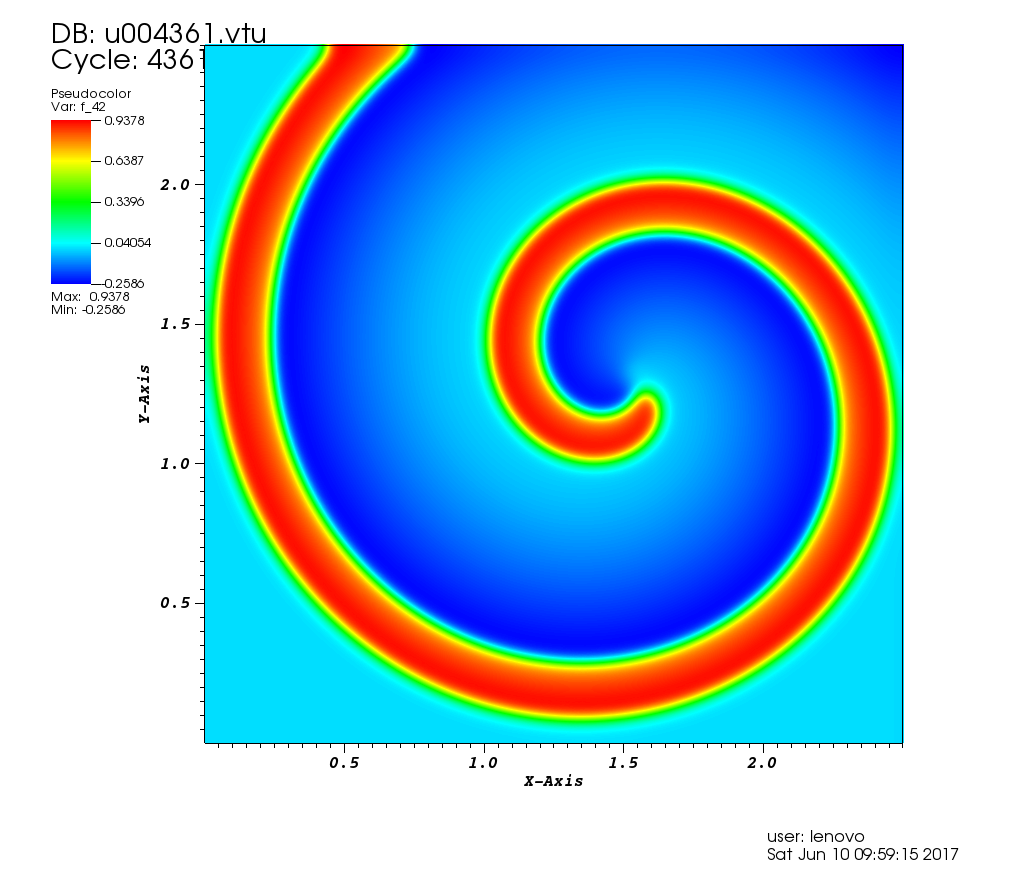
\includegraphics[width=0.25\textwidth,height=0.2\textwidth]{figures/4361.jpg}
	\hspace{0.2\textwidth}
	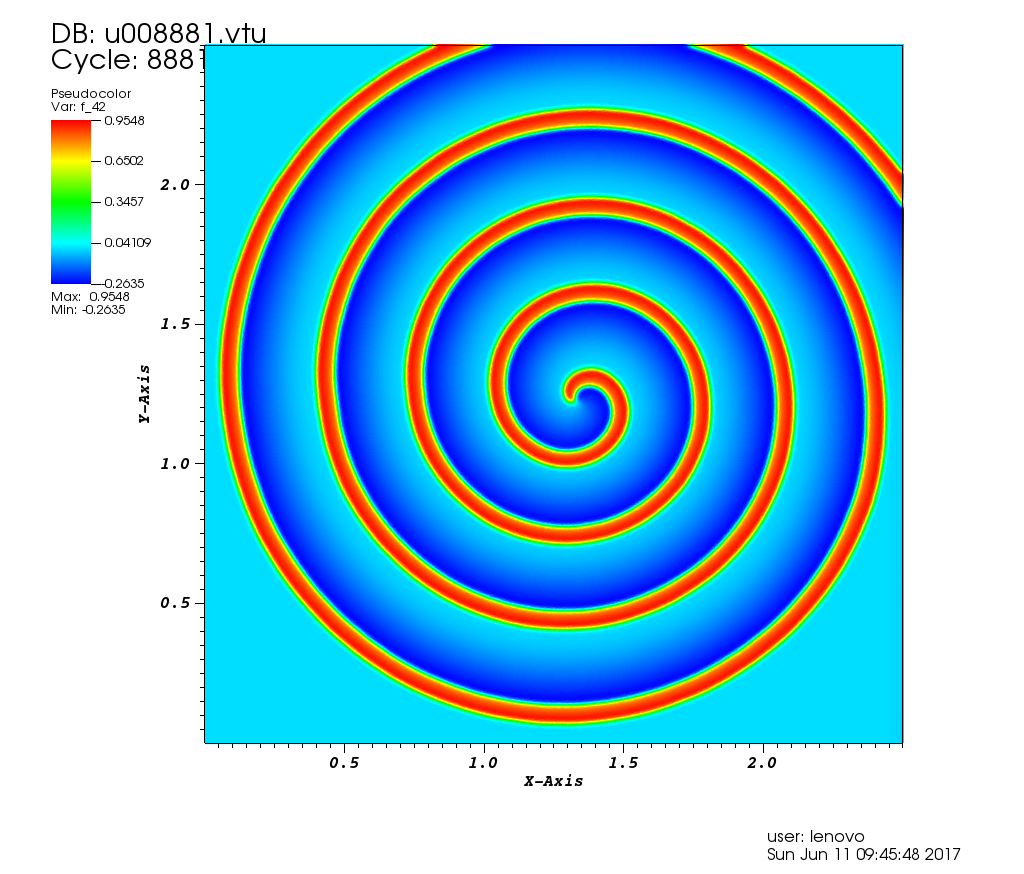
\includegraphics[width=0.25\textwidth,height=0.2\textwidth]{figures/8880.jpg}
	\hspace{0.2\textwidth}
	\subfigure[$K_x=K_y=10^{-4}$]
	{	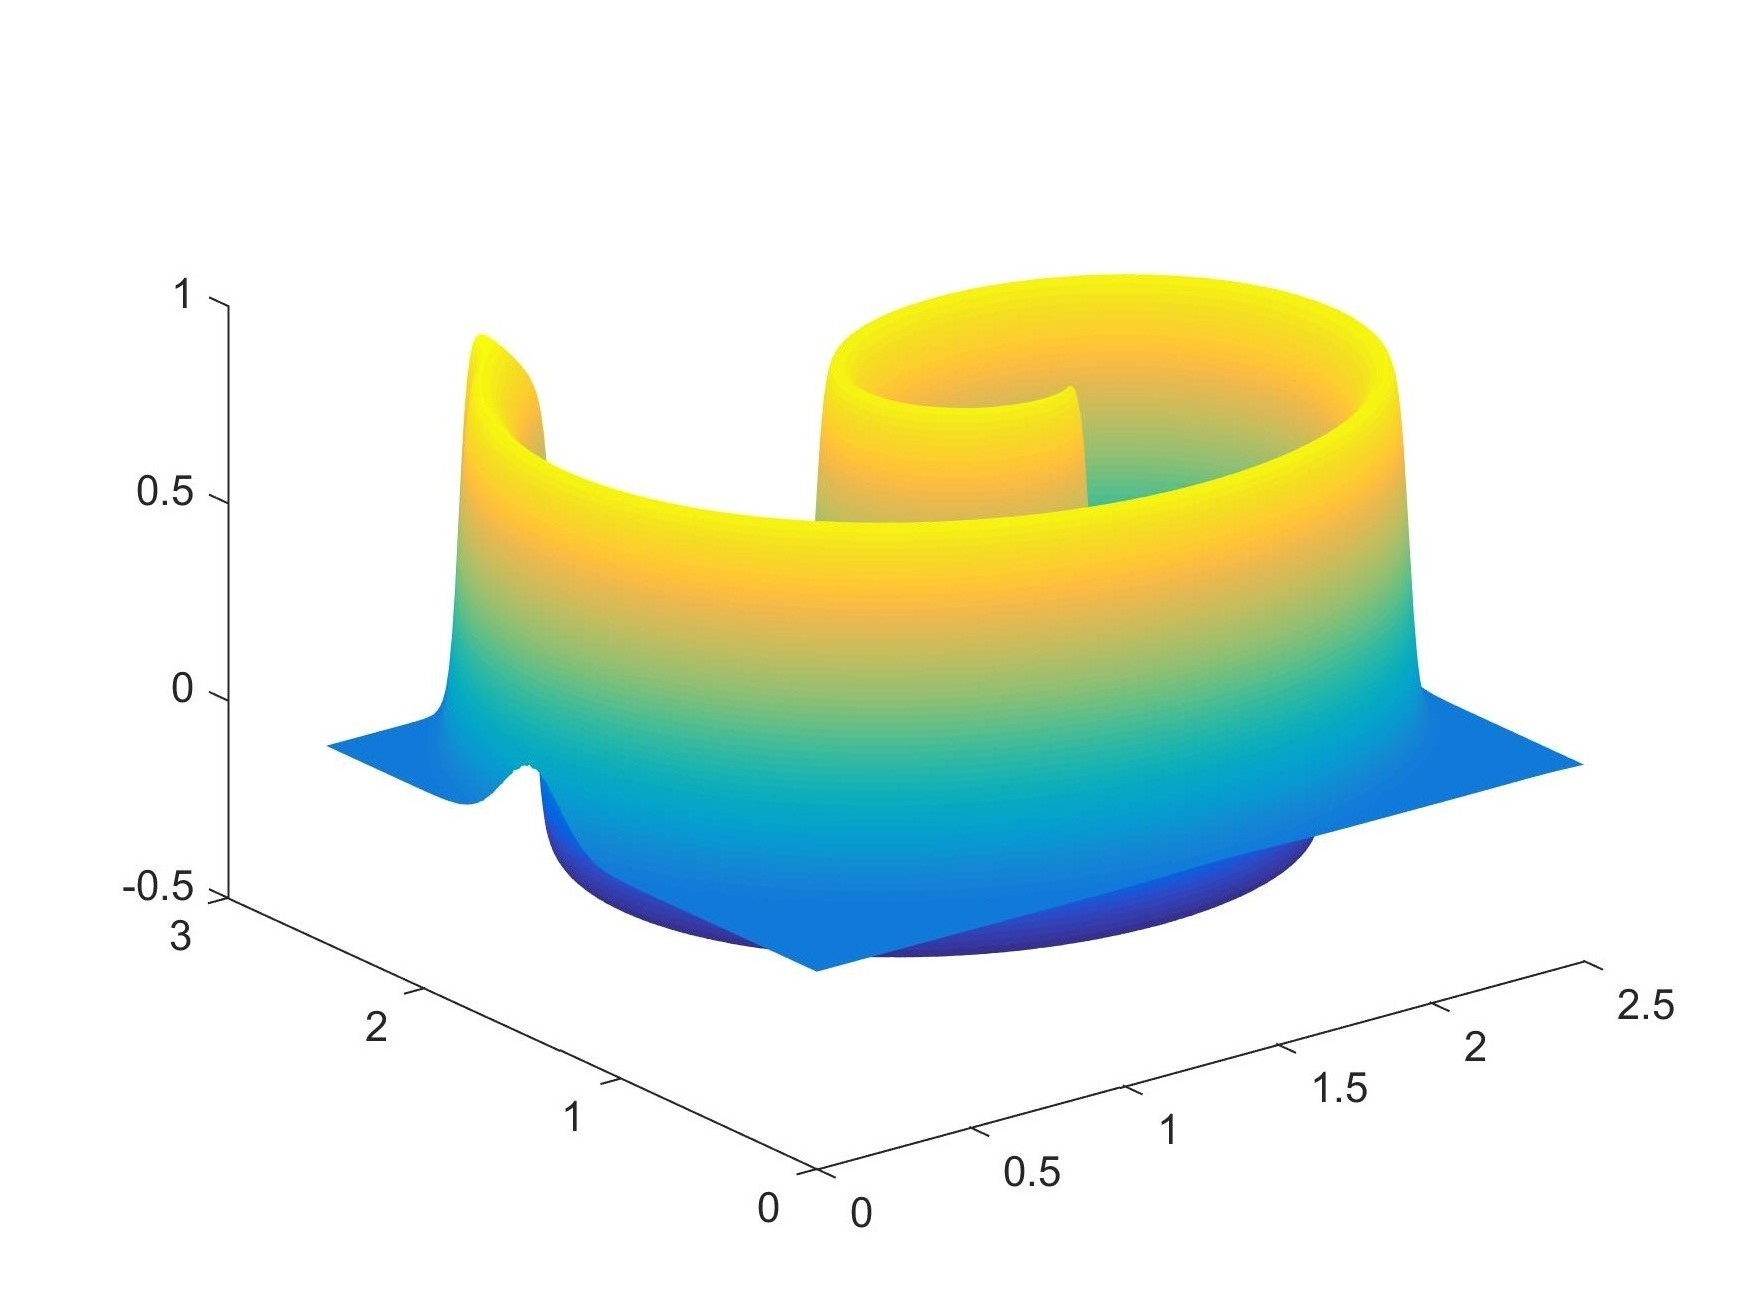
\includegraphics[width=0.25\textwidth,height=0.2\textwidth]{figures/256_p1_K_10_4.jpg}}
	\hspace{0.2\textwidth}
	\subfigure[$K_x=K_y=10^{-5}$]{	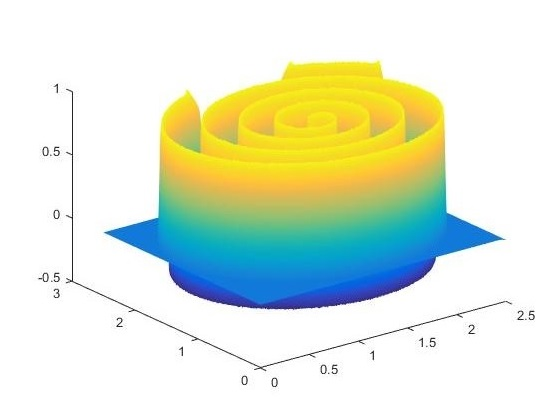
\includegraphics[width=0.25\textwidth,height=0.2\textwidth]{figures/256_p1_K_10_5.jpg}}
	\caption{二维FHN单域模型的螺旋波传播轨迹}
	\label{fig1}
\end{figure}
\begin{figure}[htb]
	\centering
	{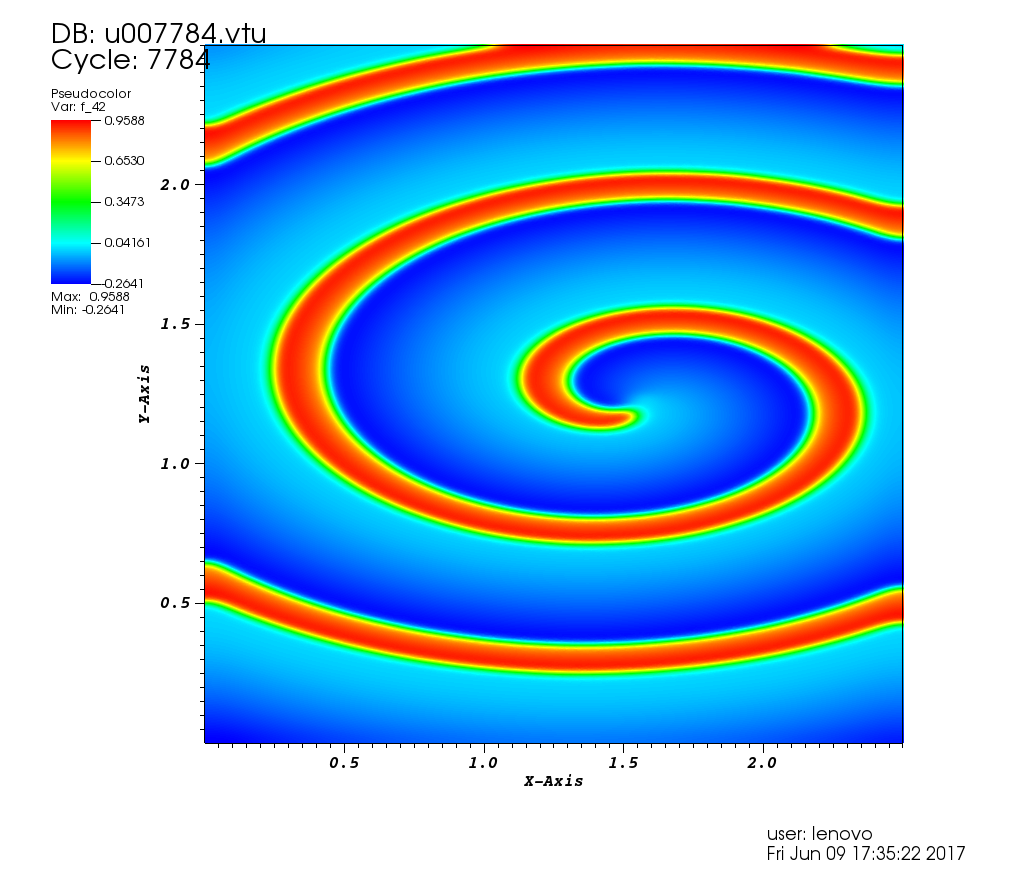
\includegraphics[width=0.25\textwidth,height=0.2\textwidth]{figures/7784.jpg}}
	\hspace{0.2\textwidth}
	{	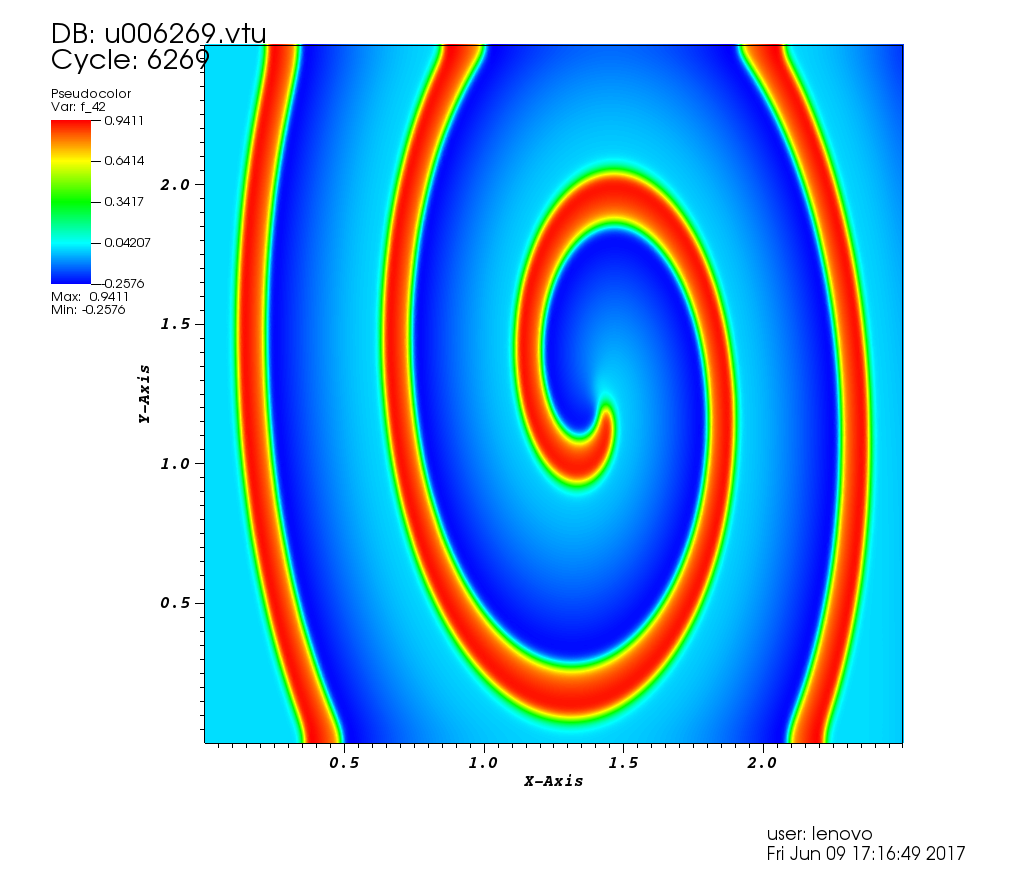
\includegraphics[width=0.25\textwidth,height=0.2\textwidth]{figures/6269.jpg}}
	\hspace{0.2\textwidth}
	\subfigure[$K_x=10^{-4},\frac{K_y}{K_x}=0.25$]
	{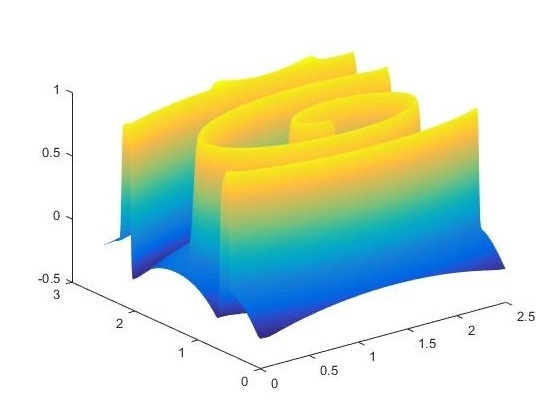
\includegraphics[width=0.25\textwidth,height=0.2\textwidth]{figures/256_p1_kx_10_4.jpg}}
	\hspace{0.2\textwidth}
	\subfigure[$K_y=10^{-4},\frac{K_x}{K_y}=0.25$]
	{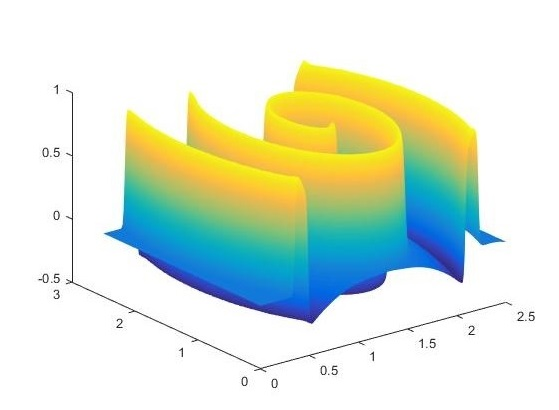
\includegraphics[width=0.25\textwidth,height=0.2\textwidth]{figures/256_p1_ky_10_4.jpg}}
	\caption{二维FHN单域模型的螺旋波传播轨迹}
	\label{fig2}
\end{figure}

\textbf{算例2}  前两个数值算例中假设外部刺激项~$I_s=0$,如果~$I_s\neq0$,通过代表性二维数值示例,可以说明导致心室颤动的心律失常的再入波的形成。再入波的形成可以具有不同的生理起源。常见的说法认为与患病心脏组织中传导特性的改变有关,例如是由心肌梗塞引起的。为了模拟心脏电生理学中螺旋波的形成和稳定的旋转,正确地捕获心脏组织的恢复特性是至关重要的。在稳定的静息组织,如心肌组织,需要两个刺激来启动重入波形。施加外部刺激的时间和区域是非常关键的。如果激发的组织样本足够大,可以启动自我持续的重入激活模式,其以高但不受控制的速率不断地重新激发自身。

考虑二维方形区域~$\Omega=\{(x,y):0\leq x\leq1, 0\leq y\leq1\}$,FHN单域模型如下形式\cite{Ying2005}
\begin{equation*}
\left\{\begin{aligned}&\frac{\partial u}{\partial t}=\varepsilon\nabla\cdot(\nabla u)+\lambda(v-u(1-u)(u-a)),\\
&\frac{\partial v}{\partial t}=\alpha u-\beta v,\end{aligned}\right.
\end{equation*}
其中~$\varepsilon=0.01$,$\lambda=-100$,$\theta=0.25$,$\alpha=0.16875$,$\beta=1.0$,选择~$T=20$,$\tau=0.01$,运用齐次Neumann边界条件,表示细胞膜和外部环境是隔绝的,并且在细胞外域边界是无通量的,初值条件~$v(x,y,0)=0$,
\begin{equation*}
u(x,y,0)=\left\{\begin{aligned}&1.0 \quad\sqrt{x^2+y^2}<0.25,\\
&0.0 \quad others,\end{aligned}\right.
\end{equation*}
在~$t=3-4$~的时间区间施加外部刺激,
\begin{equation*}
I_s=\left\{\begin{aligned}&5.0 \quad\sqrt{(x-0.5)^2+(y-0.5)^2}<0.2,\\
&0.0 \quad others,\end{aligned}\right.
\end{equation*}
结果如图~\ref{fig3}~所示,加入外部刺激后,再入波形成,并能不断地重新激发自身,循环往复。
\begin{figure}
	\centering
	{
		\subfigure[$t=2$]{
			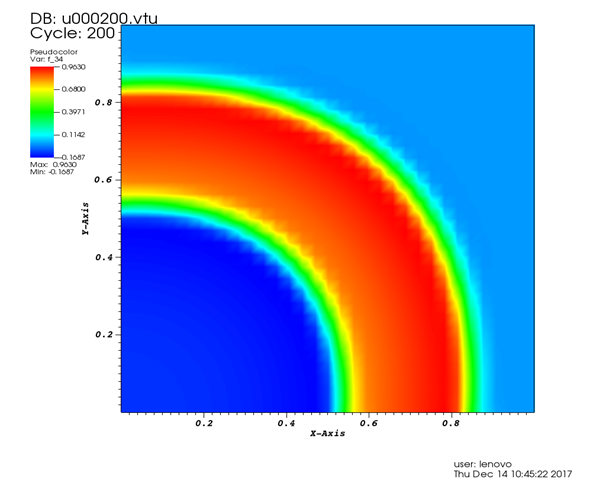
\includegraphics[width=0.3\textwidth,height=0.25\textwidth]{figures/200.png}}}
	\hspace{0.2\textwidth}
	\subfigure[$t=3.5$]{
		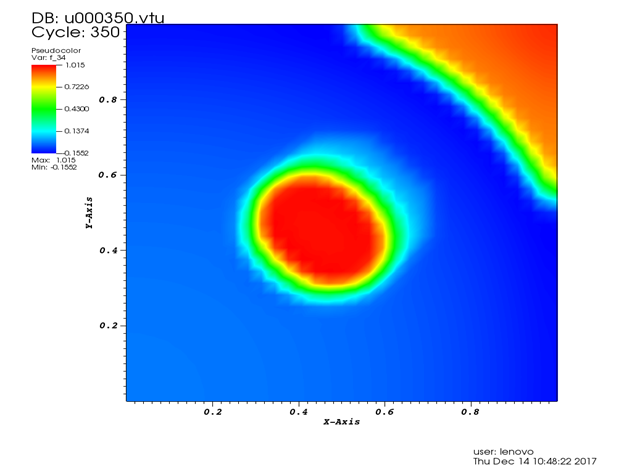
\includegraphics[width=0.3\textwidth,height=0.25\textwidth]{figures/350.png}}
	\hspace{0.2\textwidth}
	\subfigure[$t=5$]{
		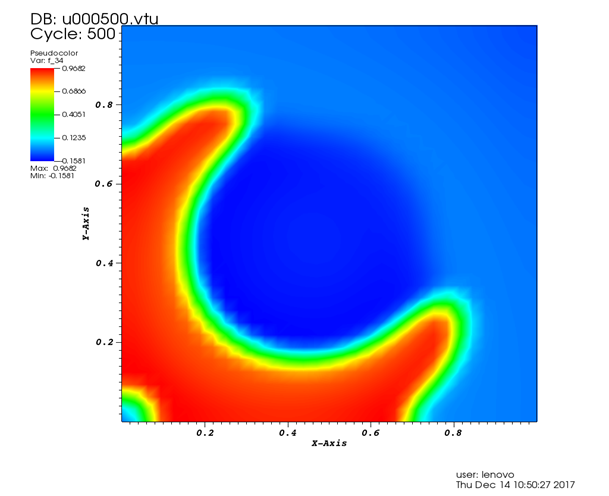
\includegraphics[width=0.3\textwidth,height=0.25\textwidth]{figures/400.png}}
	\hspace{0.2\textwidth}
	\subfigure[跨膜电势~$u$]{
		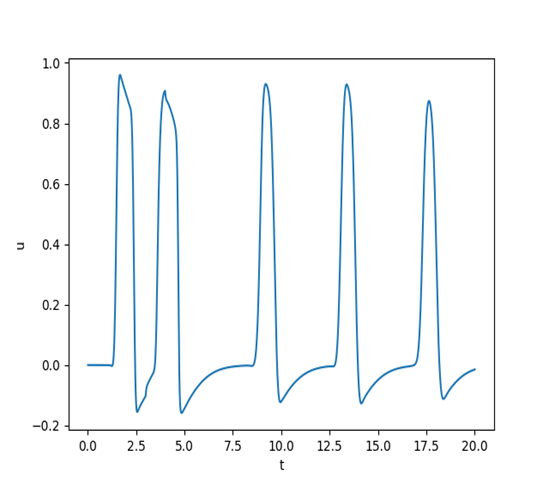
\includegraphics[width=0.3\textwidth,height=0.25\textwidth]{figures/uu.png}}
	\caption{二维FHN单域模型的跨膜电势传播状态}
	\label{fig3}
\end{figure}

\textbf{算例3} 用显-隐有限元方法,基于三维人类左心室结构求解了单域FHN模型,网格单元为四面体,控制方程同~(\ref{fhn}),选取参数~$a=0.25$,$\varepsilon=0.01$,$\beta=0.16875$,$\gamma=1$,$\delta=0$,选取时间~$T=50$,$\tau=0.5$,$K_x=K_y=K_z=1$,用齐次Neumann边界条件,初值~$v(x,y,0)=0$,并且
\begin{equation*}
u(x,y,0) =\left\{\begin{aligned}&1.0 \quad\sqrt{x-1+y-1+z-1}<3,\\
&0.0 \quad others,\end{aligned}\right.
\end{equation*}
跨膜电势的传播轨迹如图~(\ref{fig5})所示,分别表示初始状态和~$t=25$~时刻的跨膜电势传播状态。
\begin{figure}[htb]
	\centering
	{	
		\subfigure[$t=0$]{
			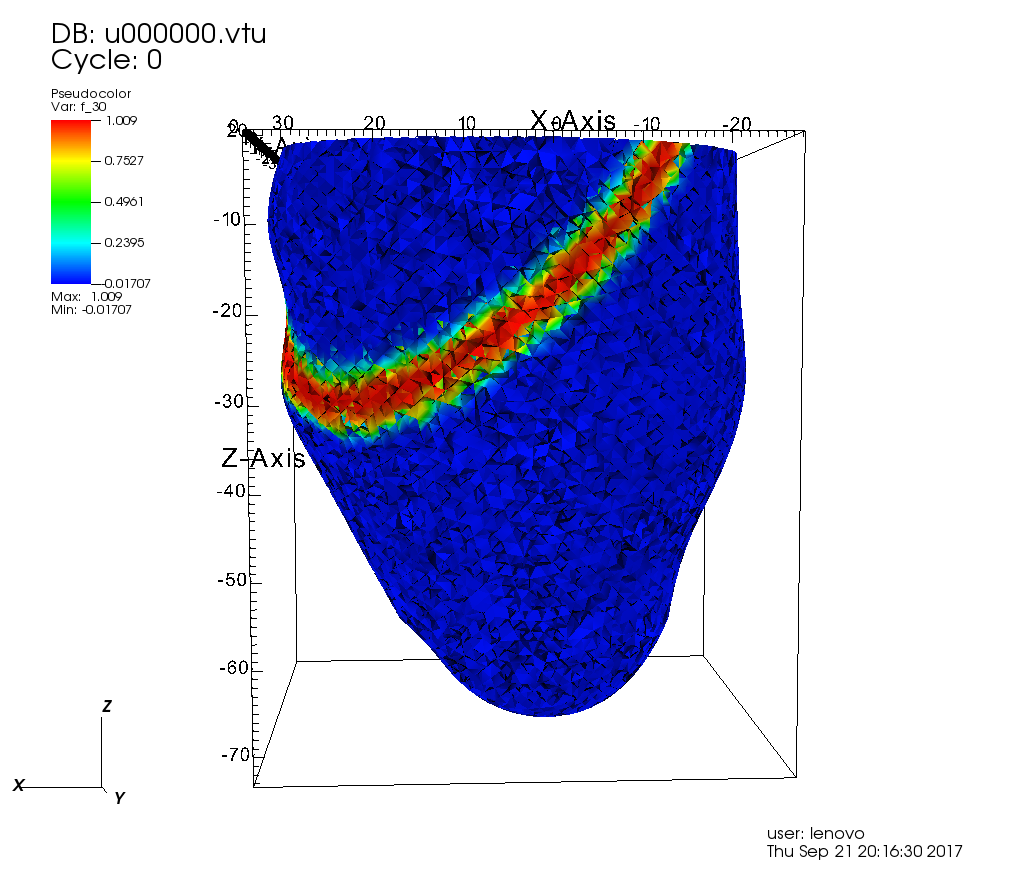
\includegraphics[width=0.25\textwidth,height=0.2\textwidth]{figures/fhn1.png}}}
	\hspace{0.2\textwidth}
	\subfigure[$t=25$]{
		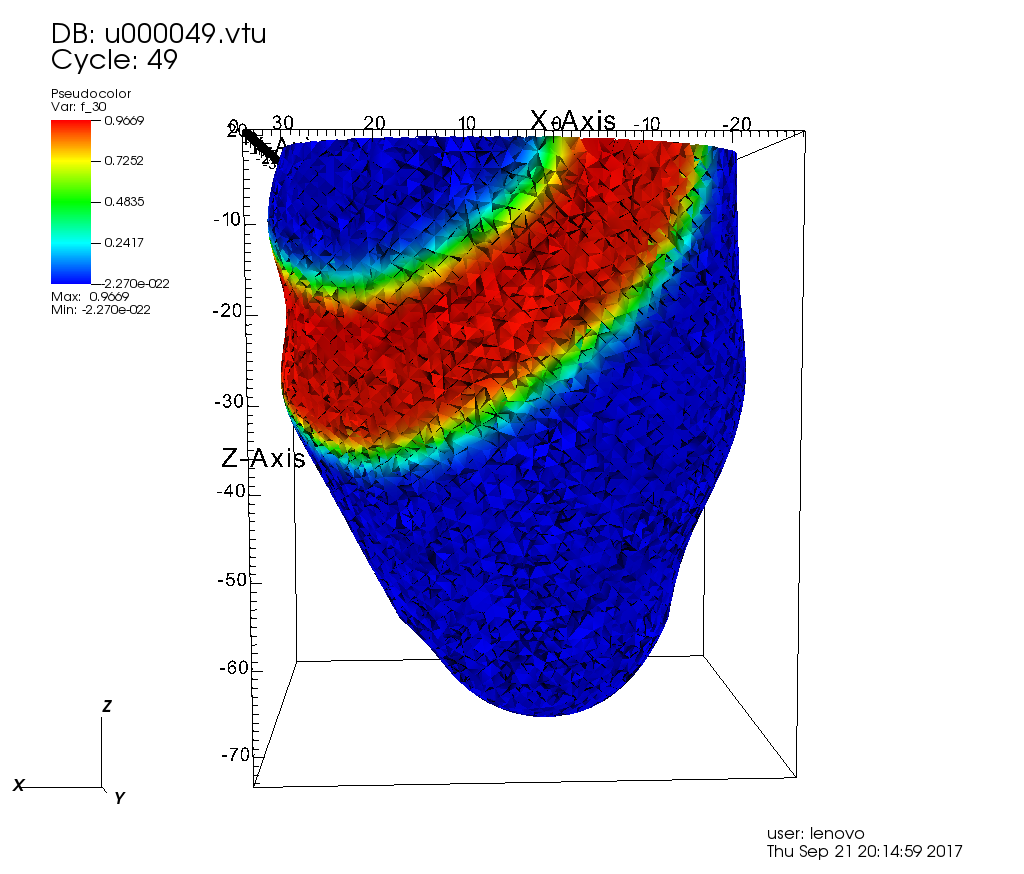
\includegraphics[width=0.25\textwidth,height=0.2\textwidth]{figures/fhn2.png}}
	\caption{三维FHN单域模型的跨膜电势传播轨迹}
	\label{fig5}
\end{figure}

\section{本章小结}
~FHN单域模型由一个反应-扩散偏微分方程和一个常微分方程耦合而成。首先基于二维FHN单域模型构造有限元离散格式,对完全离散的显-隐有限元方法进行稳定性和收敛性证明,发现当时间步长满足一定条件时,该格式稳定且收敛。本文中还将显-隐有限元方法扩展到三维情况,求解了基于三维人类左心室结构的FHN单域模型,最后用数值算例验证了显-隐有限元方法的稳定性和收敛阶,通过给定适当的初边值条件,可以观察到二维情况下FHN单域模型中螺旋波的传播状态和三维情况下跨膜电势的传播轨迹。

%==============第四章节内容==================
\chapter{FHN单域模型的算子分裂有限元方法}

在求解ODE或PDE系统时,对系统的每个部分使用同一种数值方法可能是低效的\cite{split2006}。分裂方法\cite{split2008}采用分而治之的策略,将整个系统分解为多个子系统,使得系统的某些部分可以用一种数值方法进行求解,同时系统的其他部分用另一种数值方法进行求解,从而达到更好的效果。本文利用有限元方法结合算子分裂法求解了二维和三维FHN单域模型。
\section{算子分裂方法}

算子分裂方法\cite{split2007}一般是基于整个控制方程系统,将这个系统分解为更易处理的部分,再对得到的子系统进行数值离散求解,使得求解方法具有灵活多样性,常用来求解复杂庞大的偏微分方程系统。实际研究中,由于子系统的多样性,很难对这种格式的稳定性和准确性进行严格的数学分析\cite{bodo2009}。
%但是反应项和扩散项的求解顺序和实际误差是无关的\ucite{bodo2009}。有待考证!!!
本文中的控制方程系统~(\ref{system}),运用算子分裂法,可以将该反应-扩散系统中的偏微分方程分为一个非线性常微分方程(包含反应项)和偏微分方程(包含扩散项)两部分,具体有以下形式:一个从偏微分方程分裂出来的常微分方程
\begin{equation}
\frac{\partial u}{\partial t}=I_{ion}+I_s,
\end{equation}
%\begin{equation}
%\frac{\partial v}{\partial t}=F(u,v),
%\end{equation}
以及偏微分方程
\begin{equation}
\frac{\partial u}{\partial t}=\nabla\cdot(\textbf{K}\nabla u).
\end{equation}
假设~$t_n=n\Delta t$,$u^n=u(t_n)$,$v^n=v(t_n)$~是已知的,算子分裂算法在每个时间步长需要三个步骤,并且FHN单域模型中求解常微分方程时还需要加上原控制方程~(\ref{system})中已有的线性常微分方程,具体求解过程如下:

(1)第一步在时间区间~$(t_n,t_n+\theta\Delta t]$~求解如下常微分方程初值问题:
\begin{equation*}
\left\{\begin{aligned}&\frac{\partial u}{\partial t}=I_{ion}(u,v)+I_s \quad t\in(t_n,t_n+\theta \Delta t]\quad x\in\Omega,\\& \frac{\partial v}{\partial t}=F(u,v) \quad t\in(t_n,t_n+\theta \Delta t] \quad x\in\Omega.\end{aligned}\right.
\label{1.2}
\end{equation*}
上述常微分方程的初值~$u(t_n)=u^n$,$v(t_n)=v^n$,通过求解常微分方程得到的~$t_n+\theta\Delta t$~时刻的值分别记为~$u^n_\theta$,$v^n_\theta$。

(2)第二步在时间区间~$(t_n,t_n+\Delta t]$~求解如下线性偏微分方程
\begin{equation*}
\frac{\partial u}{\partial t}=\nabla\cdot(\textbf{K}\nabla u).
\end{equation*}
上述偏微分方程的初值~$u(t_n)=u^n_\theta$,则通过求解偏微分方程得到~$t_n+\Delta t$~时刻的值记为~$u^{n+1}_\theta$。

(3)第三步在时间区间~$(t_n+\theta\Delta t,t_n+\Delta t]$~再次求解常微分方程
\begin{equation*}
\left\{\begin{aligned}&\frac{\partial u}{\partial t}=I_{ion}(u,v)+I_s \quad t\in(t_n+\theta \Delta t,t_{n+1}]\quad x\in\Omega,\\& \frac{\partial v}{\partial t}=F(u,v) \quad t\in(t_n+\theta \Delta t,t_{n+1}]\quad x\in\Omega.\end{aligned}\right.
\label{1.3}
\end{equation*}
上述常微分方程中的初值为~$u(t_n+\theta\Delta t)=u^{n+1}_\theta$,$v(t_n+\theta\Delta t,x)=v^{n}_\theta$。这一步求解得到的结果记为$u^{n+1}$,$v^{n+1}$,即为时间层~$t_n+\Delta t$~的数值解。当参数~$\theta$~取~$\frac{1}{2}$~时,为~Strang splitting,属于二阶分裂格式,当~$\theta=1$~ 时,为~Godunov splitting,属于一阶分裂格式。总的来说,二阶算子分裂过程需要求解两次常微分方程和一次偏微分方程,而一阶算子分裂过程需要求解一次常微分方程和一次偏微分方程。为了与分裂算法整体精度相适应,常微分方程和偏微分方程一般要采用和所运用算子分裂算法整体精度一致的时间离散格式。时间离散格式具体有一阶显格式,一阶隐格式,二阶Crank–Nicolson格式等离散格式。因为显格式的数值求解容易实现,但对数值格式稳定性的要求较高,而算子分裂的主要目的是降低在每个时间步骤中要求解的方程组的复杂性。所以算子分裂过程中,可以采用隐格式等时间离散格式来达到更好的数值求解效果。
\section{二维FHN单域模型变分和离散形式}

本节内容采用整体为一阶精度的Godunov splitting,即~$\theta=1$。此时只需要前两个步骤,就能得到跨膜电势~$u$~的数值解。
\subsection{变分形式}
将FHN单域模型进行算子分裂后,会有两个常微分方程和一个偏微分方程,考虑系统~(\ref{1})运用算子分裂方法后的有限元变分形式,将整个方程系统同时乘以测试函数,并将偏微分方程中的扩散项进行分部积分。有~$u(t)$,$v(t)\in U$,使得
\begin{equation}
\left\{\begin{aligned}&(u_t,p_1)=(G(u)u,p_1)-(v,p_1)\quad \forall  p_1\in V,t\in(0,T],
\\&(v_t,p_2)=\big(\varepsilon(\beta u-\gamma v-\delta),p_2\big)\quad \forall p_2\in V,t\in(0,T],
\\&(u_t,p_3)+a(u,p_3)=0\quad \forall p_3\in V,t\in(0,T],
\\&\big(u(x,y,0),p_1\big)=(u_0,p_1),\big(v(x,y,0),p_2\big)=(v_0,p_2)\quad \forall p_1,p_2\in V,\end{aligned}\right.
\label{91}
\end{equation}
成立,其中~$U=L^2(0,T;V)$,$V=H^1_0(\Omega)$~是标准的Sobolev空间。$a(u,p_3)=\int_\Omega K\nabla u\cdot\nabla p_3 dx$。
\subsection{完全离散的算子分裂有限元方法}
我们假设~$\mathcal {T}_h$~是对有界区域~$\Omega$~的三角剖分,$h$~表示所有剖分单元的最大直径。针对变分形式~(\ref{91}),将无限维的空间~$V$~中的求解问题转化为离散(有限维)空间~$V_h$~中的问题,$V_h\in V$,试探函数和测试函数空间如下
\begin{equation*}
V_h=\{p_{1h},p_{2h},p_{3h}\in H_0^1(\Omega):p_{1h},p_{2h},p_{3h}|_K\in P_s(K),\quad\forall K\in \mathcal {T}_h\},
\label{hs}
\end{equation*}
其中~$P_s(K)$~是多项式函数空间,其中最高次幂为~$s$。

记~$\tau=T/N$~为时间步长,$N$~为正整数。 $u^n_h$,$v^n_h$~是精确解~$u(t)$~和~$v(t)$~在空间~$V_h$~中,$t=t_{n}=n\tau$,($n=0,1,...,N-1$)~时刻的近似。在偏微分方程和线性常微分方程中均采用时间精度一阶隐格式,考虑到非线性常微分方程,可以将反应项按照系统~(\ref{4})中的时间离散方法进行简单线性化,在每一时间层需要求解一次常微分方程和偏微分方程,得到该时间层上~$u$~的数值解,对于~$n=0,1,...,N-1$,有~$u^{n+1}_{h*}, u^{n+1}_{h}, v^{n+1}_{h}\in V_h$,并且对~$t\in (0,T]$,$p_{1h}, p_{2h}, p_{3h}\in V_h$,使得
\begin{equation}
\left\{\begin{aligned}&(\frac{u^{n+1}_{h*}-u^n_{h}}{\tau},p_{1h})=(G(u^{n}_{h})u^{n+1}_{h*},p_{1h})-(v^n_{h},p_{1h})\quad \forall  p_{1h}\in V_h,
\\&(\frac{v^{n+1}_{h}-v^n_{h}}{\tau},p_{2h})=\big(\varepsilon(\beta u^{n+1}_{h*}-\gamma v^{n+1}_{h}-\delta),p_{2h}\big)\quad \forall p_{2h}\in V_h,
\\&(\frac{u^{n+1}_{h}-u^{n+1}_{h*}}{\tau},p_{3h})+a(u^{n+1}_{h},p_{3h})=0\quad \forall p_{3h}\in V_h,
\\&u^0_h=u_{h0}, v^0_h=v_{h0},\end{aligned}\right.
\label{92}
\end{equation}
成立,其中~$u_{h0},v_{h0}$~是初值~$u_0,v_0$~在~$V_h$~中的逼近。根据Godunov splitting算子分裂算法,求解每一时间层上的数值解,需要两个步骤。
具体每一时间层求解过程如下:

(1) 第一步在~$\Delta t$~步长求解分裂来的常微分方程和一个表示细胞膜动力学的常微分方程,初值为~$u^n_{h}$和~$v^n_{h}$,求得~$u^{n+1}_{h*}$~和~$v^{n+1}_{h}$。
\begin{equation}
\left\{\begin{aligned}&(\frac{u^{n+1}_{h*}-u^n_h}{\tau},p_{1h})=(G(u^{n+1}_{h*})u^{n}_h,p_{1h})-(v^n_h,p_{1h})\quad \forall  p_{1h}\in V_h,
\\&(\frac{v^{n+1}_{h}-v^n_{h}}{\tau},p_{2h})=\big(\varepsilon(\beta u^{n+1}_{h*}-\gamma v^{n+1}_{h}-\delta),p_{2h}\big)\quad \forall p_{2h}\in V_h,\end{aligned}\right.
\label{93}
\end{equation} 

(2) 第二步在~$\Delta t$~步长求解带有扩散项的偏微分方程,初值为第一步得到的结果~$u^{n+1}_{h*}$,求得~$u^{n+1}_{h}$。
\begin{equation}
(\frac{u^{n+1}_{h}-u^{n+1}_{h*}}{\tau},p_{3h})+a(u^{n+1}_{h},p_{3h})=0\quad \forall p_{3h}\in V_h.
\label{94}
\end{equation}

经过第二步的求解,可以最终得到~$n+1$~时间层上的数值解~$u^{n+1}_h$。
\section{三维FHN单域模型的变分和离散形式}
本节内容将二维FHN单域模型的算子分裂有限元方法扩展到三维FHN单域模型的求解中,整个反应-扩散系统的具体形式同(\ref{1}),此时~$\Omega$~表示三维区域,本文中的三维左右心室结构来自参考文献\cite{Ying2005}作者的研究成果,其利用水平集方法人工构造了左右心室三维模型,三维FHN单域模型的变分和离散形式和二维情况是一致的,在此本文中省略了数值格式的具体内容。

\section{数值算例}
本节中用有限元方法结合一阶算子分裂技术,求解了二维和三维FHN单域模型,获得了跨膜电势的传播状态。数值算例中均采用线性拉格朗日基函数,并且用运用基于多重网格(AMG)预条件的稳定双共轭梯度法,求解线性代数方程组系统。

\textbf{算例~I} 选择~$T=1000$,时间步长~$\tau=0.1$,$K=\left(\begin{array}{cc}K_x & 0 \\0 & K_y \\ \end{array}\right)$。初值条件同~(\ref{bound}),考虑Dirichlet边界条件~$u|_{\partial\Omega}=0$,$ v|_{\partial\Omega}=0$。当~$K_x=K_y=10^{-4}$~时,螺旋波的传播轨迹在如图~\ref{fig4} (a) 所示。当~$K_x=10^{-4}$,$\frac{K_y}{K_x}=0.25$~时,模拟结果如图~\ref{fig4}(b)所示。这些结果和文献\cite{fw2012}中的结果一致,能证实算子分裂方法结合有限元方法的稳定性。
\begin{figure}[htb]
	\centering
	{	
		\subfigure[$K_x=K_y=10^{-4}$]{
			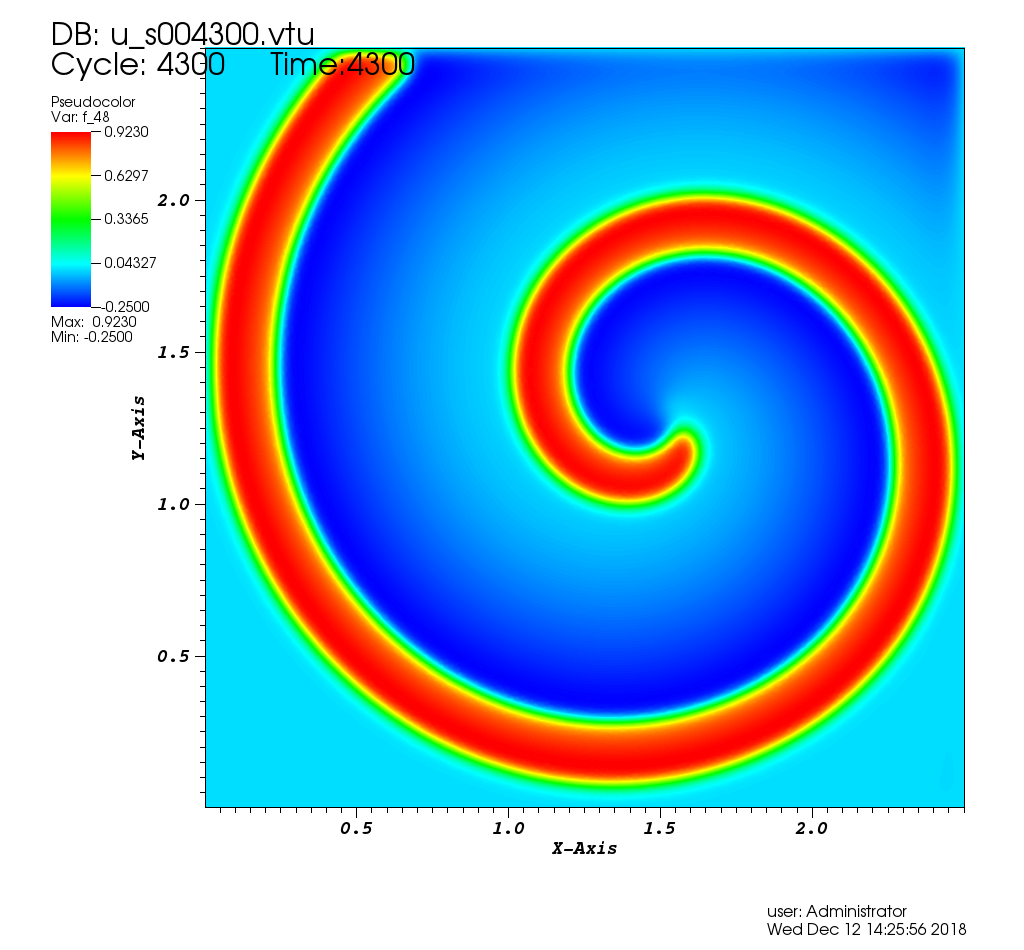
\includegraphics[width=0.25\textwidth,height=0.2\textwidth]{figures/split1.png}}}
	\hspace{0.2\textwidth}
	\subfigure[$K_x=10^{-4}, \frac{K_y}{K_x}=0.25$]{
		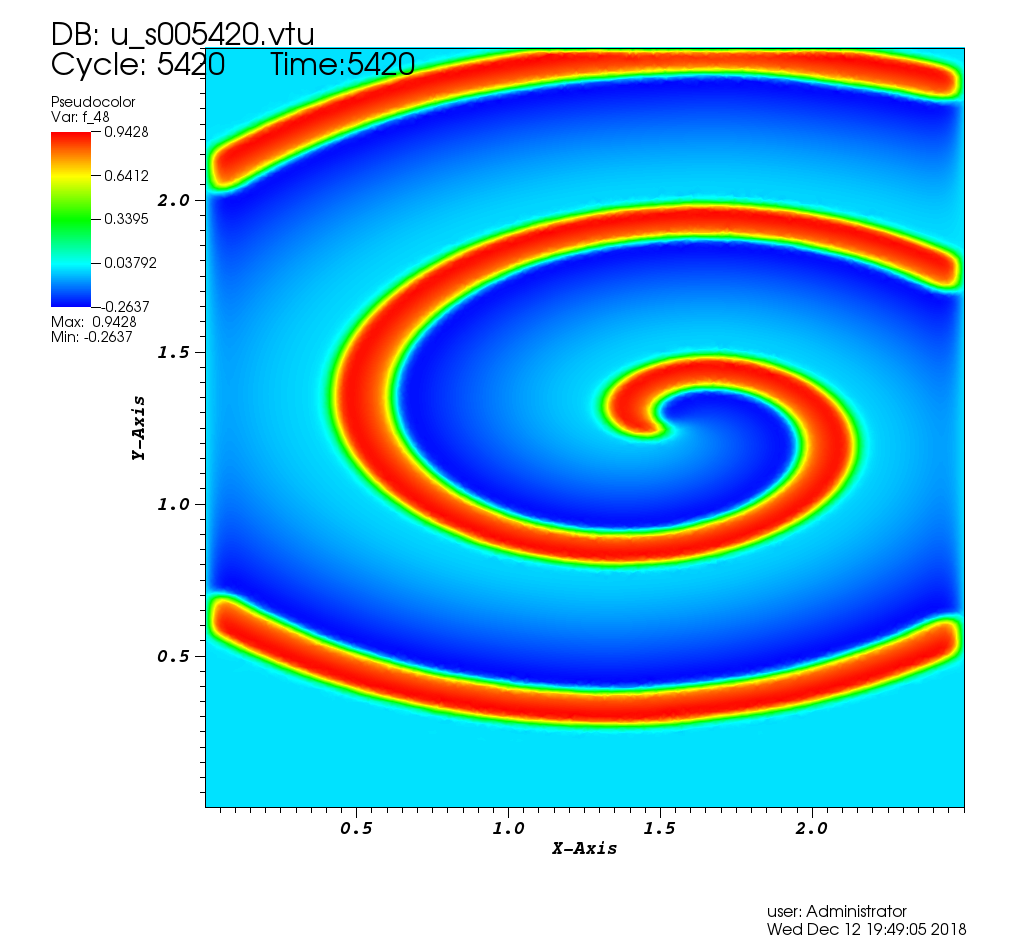
\includegraphics[width=0.25\textwidth,height=0.2\textwidth]{figures/split2.png}}
	\caption{二维FHN单域模型中螺旋波的传播轨迹}
	\label{fig4}
\end{figure}

\textbf{算例~II} 用算子分裂有限元方法,基于三维左右心室结构求解了FHN单域模型,网格单元为四面体,控制方程同~(\ref{1}),选取参数~$a=0.25$,$\varepsilon=0.01$,$\beta=0.16875$,$\gamma=1$,$\delta=0$,选取时间~$T=50$,$\tau=0.1$,$K_x=K_y=K_z=0.01$,用齐次Neumann边界条件,初值~$v(x,y,0)=0$,并且
\begin{equation*}
u(x,y,0) =\left\{\begin{aligned}&1.0 \quad\sqrt{x-0.8+y-0.9+z-1}>0.6,\\
&0.0 \quad others,\end{aligned}\right.
\end{equation*}
跨膜电势的传播轨迹如图~\ref{fig7}~所示,分别表示初始状态以及~$t=10$,$t=15$,$t=20$~时刻的跨膜电势传播趋势。
\begin{figure}[htb]
	\centering
	{	  \subfigure[$t=0$]{
			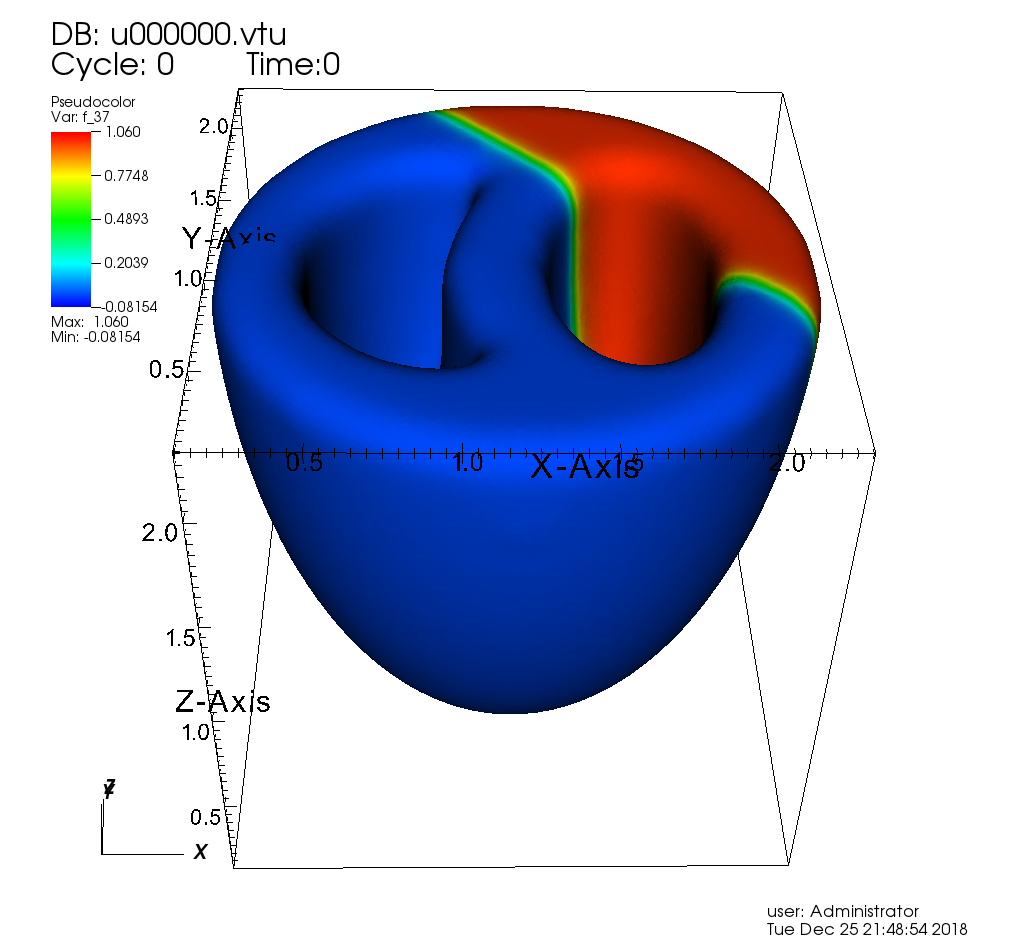
\includegraphics[width=0.3\textwidth,height=0.3\textwidth]{figures/3d0.png}}}
	\hspace{0.2\textwidth}
	\subfigure[$t=10$]{
		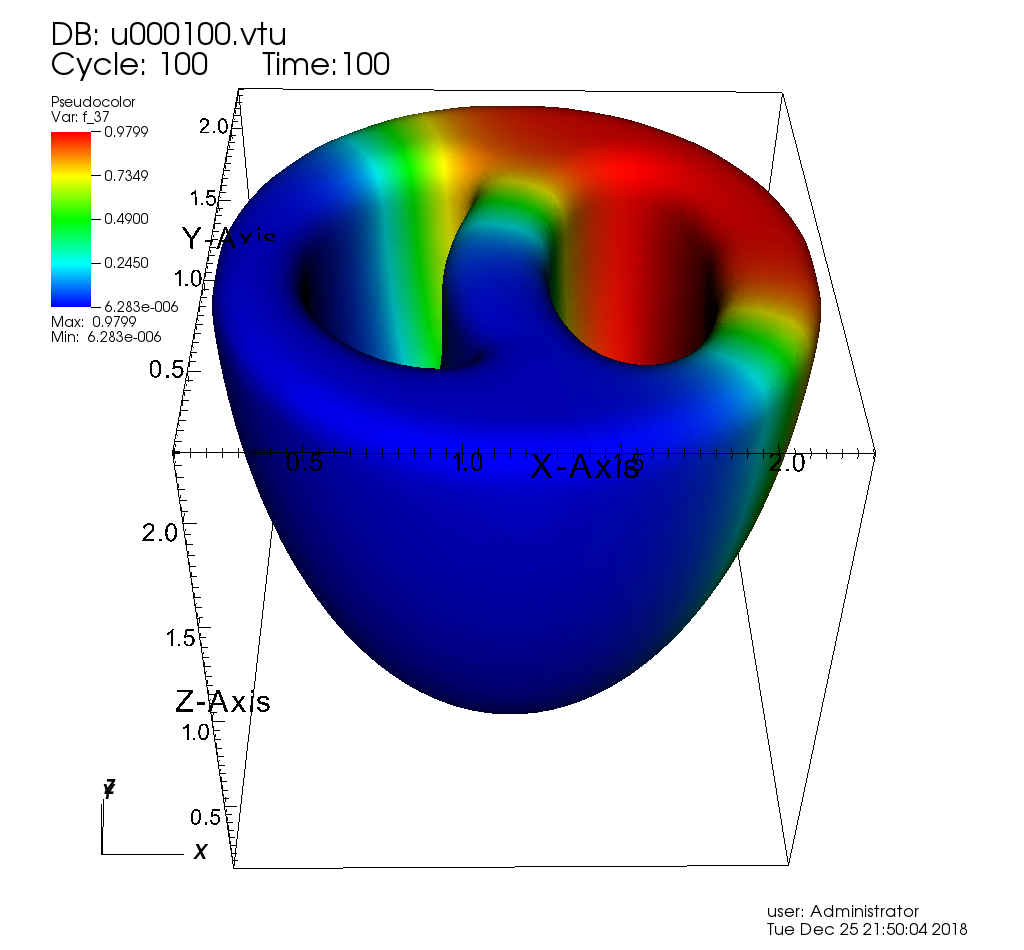
\includegraphics[width=0.3\textwidth,height=0.3\textwidth]{figures/3d2.png}}
	\hspace{0.2\textwidth}
	\subfigure[$t=15$]{
		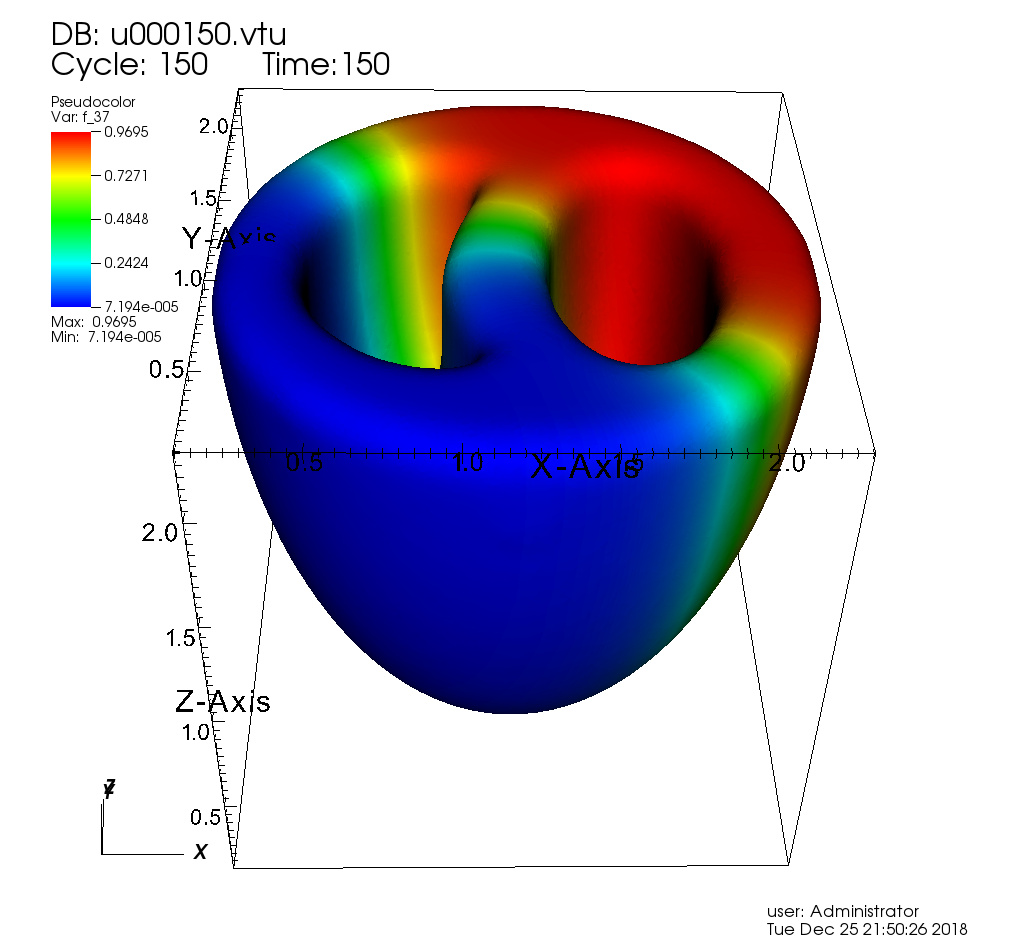
\includegraphics[width=0.3\textwidth,height=0.3\textwidth]{figures/3d3.png}}
	\hspace{0.2\textwidth}
	\subfigure[$t=20$]{
		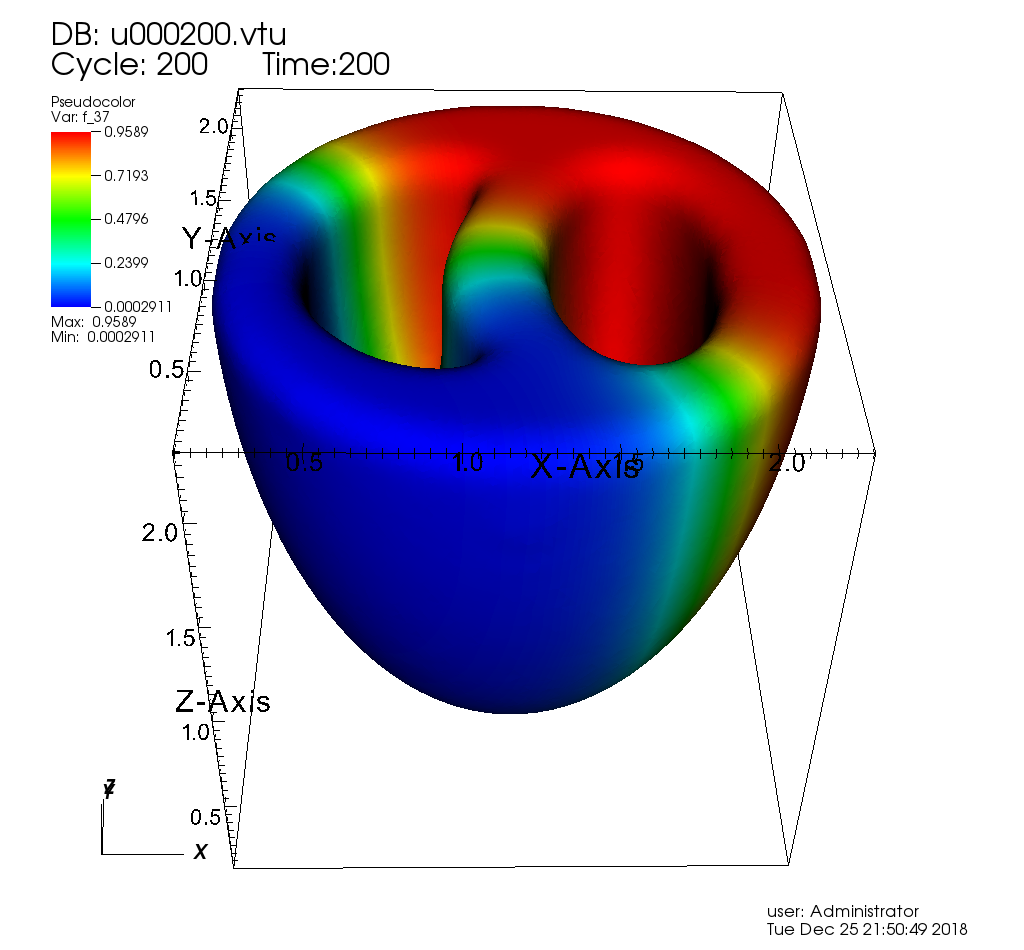
\includegraphics[width=0.3\textwidth,height=0.3\textwidth]{figures/3d4.png}}
	\caption{三维FHN单域模型跨膜电势的传播轨迹}
	\label{fig7}
\end{figure}
\section{本章小结}
本节主要基于有限元方法结合算子分裂技术,求解了FHN单域模型。给出了二维FHN单域模型的时间-空间完全离散格式,每个时间层上需要求解一次常微分方程系统和一次偏微分方程,得到跨膜电势~$u$~的数值解。将该方法扩展到三维FHN单域模型的数值计算中。因为算子分裂方法得到的子系统比较复杂,我们没有给出相关的稳定性和收敛性的理论证明。最后通过数值算例,给定合适的初边值条件,二维情况下得到了稳定的螺旋波传播轨迹,三维情况下可以得到跨膜电势的传播状态。

%==============第五章节内容==================
\chapter{ORd单域模型的算子分裂有限元方法}

一般认为,室性心律失常的维持可能受到心室心肌的复杂三维结构以及动作电位特征的空间不均匀性的影响。因此,借助计算机技术进行数学建模时,应该在模型中结合重要的解剖学特征,使得能够以准确和有效的方式表示心室心肌的不均匀和各向异性的电特性。
O’Hara-Rudy dynamic(ORd)单细胞模型是由O’Hara T等人于2010年基于非病态的人类心室数相关据开发出来的动作电位模型,这个动作电位模型更具有现实意义,因为现有的一些模型大多是基于非心肌细胞的,或者实验数据来自于动物等非人心肌细胞,这导致模型的不严谨性。ORd模型结合人类心室真实的实验数据,并且对心脏电活动至关重要的离子通道动力学,特别是~$Ca^{2+}$~有了新的发现,最终得到了描述真实人类心室肌细胞电生理学的ORd单细胞模型。根据电生理学的性质,通过修改ORd单细胞模型中与离子流相关的参数,能够用来模拟三种类型的心肌细胞,分别是心内膜细胞,心肌中部的细胞,心外膜细胞\cite{ord1}。本文中基于三维左右心室结构,用有限元方法结合一阶算子分裂(Godunov splitting)方法求解了ORd 单域模型。
\section{控制方程}
ORd单域模型的控制方程形式如下:
\begin{equation}
\left\{\begin{aligned}&\frac{\partial u}{\partial t}=\nabla\cdot(\textbf{K}\nabla u)-C_m^{-1}(I_{ion}(u,\textbf{v},\textbf{w})-I_s)\quad (\textbf{x},t)\in\Omega\times(0,T],
\\&\frac{\partial \textbf{v}}{\partial t}=F(u,\textbf{v}) \quad(\textbf{x},t)\in\Omega\times(0,T],
\\&\frac{\partial \textbf{w}}{\partial t}=S(u,\textbf{v},\textbf{w})\quad(\textbf{x},t)\in\Omega\times(0,T],
\\&u_0=u(\textbf{x},0),\textbf{v}_0=\textbf{v}(\textbf{x},0),\textbf{w}_0=\textbf{w}(\textbf{x},0)\quad \textbf{x}\in\Omega,
\\&\frac{\partial u}{\partial \textbf{n}}=0 \quad(\textbf{x},t)\in\partial\Omega\times (0,T).\end{aligned}\right.
\label{ORD}
\end{equation}
这是一个有量纲的反应-扩散系统,$\Omega\in R^3$,$\textbf{x}=(x,y,z)$,$u$~表示跨膜电势(mV),$\textbf{v}\in R^p$~表示控制离子通道的激活和失活的门控因子,$\textbf{w}\in R^q$~ 表示离子浓度相关的变量,表征心肌细胞的生理状态,$C_m$~表示细胞膜电容($\mu F$),包含14种离子流的总电流$I_{ion}=I_{Na}+I_{to}+I_{CaL}+I_{CaNa}+I_{CaK}+I_{Kr}+I_{Ks}+I_{K1}+I_{NaCa}+I_{NaK}+I_{Nab}+I_{Cab}+I_{Kb}+I_{pCa}$,单位均为mM,其中~$I_{Na}$~为~$Na^+$~离子流,$I_{to}$~为瞬态外向~$K^+$~电流,$I_{CaL}$~表示通过~$L$~类型的~$Ca^{2+}$~通道的~$Ca^{2+}$~电流,$I_{CaNa}$~为通过~$L$~类型的~$Ca^{2+}$~通道的~$Na^+$~电流,$I_{CaK}$~表示通过~$L$~类型的~$Ca^{2+}$~ 通道的~$K^+$电流,$I_{Kr}$~为快速延迟整流~$K^+$~电流,$I_{Ks}$~为慢延迟整流~$K^+$~电流,$I_{K1}$~为内向整流~$K^+$~离子流,$I_{NaCa}$~是总~$Na^+/Ca^{2+}$~交换电流,$I_{NaK}$~为~$Na^+ / K^+ ATPase$ ~电流,$I_{Kb}$~表示~$K^+$ 背景电流,$I_{pCa}$~表示肌纤维膜~$Ca^{2+}$~泵电流。$F(u,\textbf{v})$~由离子流决定,该模型涉及40个常微分方程,$I_s$~表示外部刺激($\mu A/\mu F$)。
描述人类心室动作电位的动力学机制如图(\ref{fig:1.1})所示。
\begin{figure}[ht]
	\centering
	%\subfigure[心肌细胞]{
	%\label{fig:subfig:cell}
	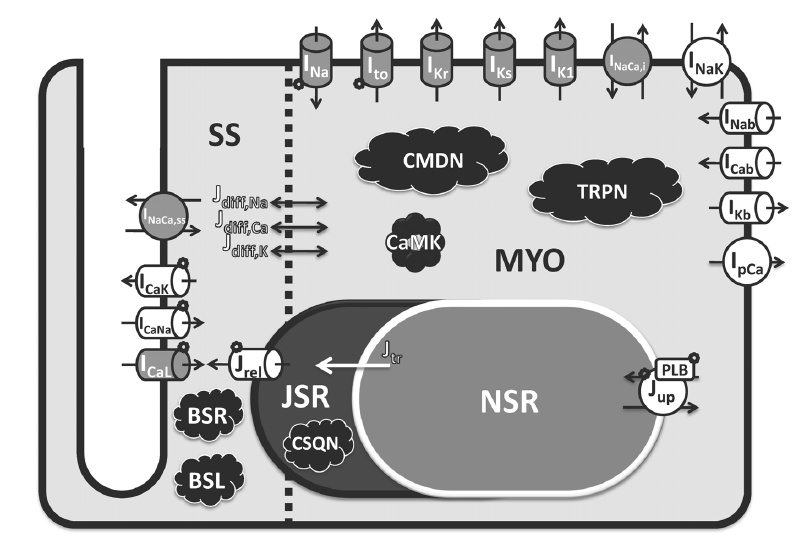
\includegraphics[width=0.8\textwidth,height=0.5\textwidth]{figures/liziliu.PNG}
	\hspace{0.04\textwidth}
	%\subfigure[细胞膜]{
	%\label{fig:subfig:membrane}
	%\includegraphics[width=0.25\textwidth,height=0.3\textwidth]{fig/membrane}}
	\caption{人类心室肌细胞动作电位模型\cite{ORD2011}}
	\label{fig:1.1} %% label for entire figure
\end{figure}
$Na^{+}$~电流在除极阶段以较快的速度激活又以很快的速度失活,这个过程导致动作电位的上升期,$Ca^{2+}$~电流的激活和失活速度都比~$Na^{+}$~缓慢,动作电位的平台期主要由~$Ca^{2+}$~来维持,$K^{+}$~电流激活速度是最慢的,它的外流导致膜电位处于最终复极化阶段。本文考虑到所有离子流涉及到的公式比较冗长,为了表达直观,主要给出了~$I_{Kr}$~ 离子电流的具体形式,具体模型参数可见参考文献\cite{ORD2011}。
\begin{equation*}
x_{r,\infty}=\frac{1}{1+exp(\frac{-(V+8.337)}{6.789})},
\end{equation*}
\begin{equation*}
\tau_{x,r,fast}=12.98+\frac{1}{0.3652\cdot exp(\frac{V-31.66}{3.869})+4.123\cdot10^{-5}\cdot exp(\frac{-(V-47.78)}{20.38})},
\end{equation*}
\begin{equation*}
\tau_{x,r,slow}=1.865+\frac{1}{0.06629\cdot exp(\frac{V-34.70}{7.355})+1.128\cdot10^{-5}\cdot exp(\frac{-(V-29.74)}{25.94})},
\end{equation*}
\begin{equation*}
A_{x,r,fast}=\frac{1}{1+exp(\frac{V+54.81}{38.21})},\quad A_{x,r,slow}=1-A_{x,r,fast},
\end{equation*}
\begin{equation}
\frac{dx_{r,fast}}{dt}=\frac{x_{r,\infty}-x_{r,fast}}{\tau_{x,r,fast}}, \quad \frac{dx_{r,slow}}{dt}=\frac{x_{r,\infty}-x_{r,slow}}{\tau_{x,r,slow}},
\label{rh}
\end{equation}
\begin{equation*}
x_r=A_{x,r,fast}\cdot x_{r,fast}+A_{x,r,slow}\cdot x_{r,slow},
\end{equation*}
\begin{equation*}
R_{Kr}=\frac{1}{\big(1+exp(\frac{V+55}{75})\big)\big(1+exp(\frac{V-10}{30})\big)},
\end{equation*}
\begin{equation*}
I_{Kr}=\overline{G_{Kr}}\cdot \sqrt{\frac{[K^+]_o}{5.4}}\cdot x_r\cdot R_{Kr}\cdot (V-E_K),
\end{equation*}
其中~$V$~为跨膜电势,$[K^+]_o=5.4mM$~为~$K^+$~的外部浓度,
\begin{equation*}
E_{K}=\frac{RT}{F}\cdot ln(\frac{[K^+]_o}{[K^+]_i}),
\end{equation*}
$R=8314~J/kmol/K$~表示气体常数,$T=310^\circ$~表示温度,$F=96485~coul/mol$~表示法拉第常数,$x_{r,fast}$,$x_{r,slow}$~分别表示与~$I_{Kr}$~有关的快速激活和失活状态的门控变量,慢速激活和失活状态的门控变量。$[K^+]_i$~表示与~$K^+$~相关的离子浓度,初值为143.79mM,离子浓度变量~$[K^+]_i$~也会涉及一个与时间相关的常微分方程:
\begin{equation*}
\frac{d[K^+]_i}{dt}=-(I_{to}+I_{Kr}+I_{Ks}+I_{K1}+I_{Kb}+I_{stim}-2I_{NaK})\cdot\frac{A_{cap}}{F\cdot v_{myo}}+J_{diff,Na}\cdot\frac{v_{ss}}{v_{myo}},
\end{equation*}
其中~$I_{stim}$~表示刺激电流($\mu A/\mu F$),
\begin{equation*}
J_{diff,K}=\frac{[K^+]_{ss}-[K^+]_i}{\tau_{diff,K}},
\end{equation*}
其表示扩散通量,$\tau_{diff,K}=2.0~ms$~,$A_{cap}=1.534\cdot10^{-4}~cm^2$~表示电容面积,
$[K^+]_{ss}$~也是一个离子浓度相关的变量,初值为143.79~$mM$,满足
\begin{equation*}
\frac{d[K]_{ss}}{dt}=-I_{CaK}\cdot\frac{A_{cap}}{F\cdot v_{ss}}-J_{diff,K},
\end{equation*}
$v_{myo}=25.84\cdot10^{-6}~\mu L$~和~$v_{ss}=0.76\cdot10^{-6}~\mu L$~均表示与细胞几何相关的常量。可以看出这些常微分方程是相互影响的。


\section{三维ORd单域模型的变分和离散形式}
本文中用了有限元方法结合一阶算子分裂格式求解了ORd单域模型,即~$\theta=1$~时,将控制系统分为一个偏微分方程和一个常微分方程系统,整个过程中在每个时间步长,需要求解一次常微分方程系统和一次偏微分方程。
偏微分方程的时间离散采用隐格式,描述门控变量的常微分方程系统采用RH方法\cite{RL1978,RL1985},这是解决描述心肌细胞模型动态行为所涉及的常微分方程比较常用的方法之一。非门控变量相关的常微分方程也采用隐格式进行时间离散。

该系统中涉及的常微分系统可以先简化为如下初边值问题
\begin{equation}
\frac{d\textbf{y}}{dt}=f(t,\textbf{y}),\quad \textbf{y}(t_n)=\textbf{y}_n,
\end{equation}
其中~$\textbf{y}$~代表多个状态变量的矢量,这些变量包括门控变量(描述细胞膜对不同离子流的通透性)和一些离子浓度相关的变量,门控变量相关的常微分方程,例如方程(\ref{rh}),有以下形式
\begin{equation}
\frac{dy}{dt}=\frac{y_\infty-y}{\tau_y},
\end{equation}
其中~$y_\infty=\frac{\alpha_y}{\alpha_y+\beta_y}$,$\tau_y=\frac{1}{\alpha_y+\beta_y}$,并且~$\alpha_y$~和~$\beta_y$~是与跨膜电势~$u$~相关的速率常数,$\alpha_y=\alpha_y(u)$,$\beta_y=\beta_y(u)$,RH方法假设在每一个时间步长求解时,跨膜电势~$u$~是一个常数。上述方程可以写成
\begin{equation}
y_n=y_\infty+(y_{n-1}-y_\infty)e^{-\frac{\Delta t_n}{\tau_y}} \quad \Delta t_n=t_{n+1}-t_n.
\end{equation}

%求解过程:ovvr.py,即膜模型部分,主要分为四个函数,第一个函数包含所有参数常量,第二个函数包含所有变量(跨膜电势和状态变量)的初值,第三个函数列出来每个离子流$in$的表达式,并且不会涉及常微分方程的离散和表示,只是和常微分相关的变量名用第二个函数中的“初值”名直接代替,返回值为$I_{ion}=i1+i2+...in+is$~即离子流部分。第四个函数就是所有常微分系统(40个)的右端项表达式。并且返回这40个右端项组成的向量。
\subsection{变分形式}
考虑系统(\ref{ORD})在三维情况下运用算子分裂方法后的有限元变分形式,将ORd单域模型进行算子分裂后,会有一个常微分系统和一个偏微分方程,首先明确跨膜电势~$u$~是一个标量,$u\in U$,门控变量~$\textbf{v}\in P$,离子浓度~$\textbf{w}\in Q$,
\begin{equation}
\left\{\begin{aligned}&(u_t,p_1)=-C_m^{-1}\big(I_{ion}(u,\textbf{v}),p_1)-(I_s,p_1)\big) \quad \forall  p_1\in U,  t\in(0,T],
\\&(\textbf{v}_t,p_2)=\big(F(u,\textbf{v}),p_2\big)\quad \forall p_2\in P, t\in(0,T],
\\&(\textbf{w}_t,p_3)=\big(S(u,\textbf{v},\textbf{w}),p_3\big)\quad \forall p_3\in Q, t\in(0,T],
\\&(u_t,p_3)+a(u,p_4)=0\quad \forall p_4\in U,t\in(0,T],
\\&\big(u(\textbf{x},0),p_1\big)=(u_0,p_1),\big(\textbf{v}(\textbf{x},0),p_2\big)=(\textbf{v}_0,p_2),\big(\textbf{w}(\textbf{x},0),p_2\big)=(\textbf{w}_0,p_3).
%\forall p_1,p_2,p_3\in U.
\end{aligned}\right.
\label{01}
\end{equation}
成立,其中~$U=L^2(0,T;V)$,$V=H^1(\Omega)$~是标准的Sobolev空间。$P=L^2(0,T;X_1)$,\\
$X_1=L^2(\Omega)^{p}$,$Q=L^2(0,T,X_2)$,$X_2=L^2(\Omega)^q$,$a(u,p_4)=\int_\Omega K\nabla u\cdot\nabla p_4dx$。
\subsection{完全离散的算子分裂有限元方法}
我们假设~$\mathcal {T}_h$~是对有界区域~$\Omega$~的剖分,$h$~表示所有剖分单元的最大直径。针对变分形式~(\ref{01}),将无限维的空间~$V$,$X_1$,$X_2$~中的求解问题转化为离散(有限维)空间~$V_h$,$X_{1h}$,$X_{2h}$~中的问题,$V_h\in V$,$X_{1h}\in X_1$,$X_{2h}\in X_2$。
%试探函数和测试函数空间如下
%\begin{equation*}
%V_h=\{p_{1h},p_{4h}\in H^1(\Omega):p_{1h},p_{4h}|_K\in %P_s(K),\quad\forall K\in \mathcal {T}_h\},
%\end{equation*}
%\begin{equation*}
%X_{1h}=\{p_{2h}\in L^2(\Omega)^{p}:p_{2h}|_K\in P_s(K),\quad\forall K\in %\mathcal {T}_h\},
%\label{0hs}
%\end{equation*}
%\begin{equation*}
%X_{2h}=\{p_{3h}\in L^2(\Omega)^{q}:p_{3h}|_K\in P_s(K),\quad\forall K\in %\mathcal {T}_h\},
%\label{0hs}
%\end{equation*}
%其中~$P_s(K)$~是多项式函数空间,其中最高次幂为~$s$。

记~$\tau=T/N$~为时间步长,$N$~为正整数。$u^n_h$,$\textbf{v}^n_h$,$\textbf{w}^n_h$~分别是精确解~$u(t)$,$\textbf{v}(t)$~和~$\textbf{w}(t)$~在空间~$V_h$,$X_{1h}$,$X_{2h}$~中,$t=t_{n}=n\tau$,($n=0,1,...,N-1$)时刻的近似。在偏微分方程中用向后欧拉时间离散隐格式,常微分方程系统中门控变量用RL 方法处理,离子浓度变量等非门控变量也用隐格式处理,运用一阶算子分裂技术的完全离散的有限元方法就是对于~$n=0,1,...,N-1$,有~$u^{n+1}_h, u^{n+1}_{h*}\in V_h$,$\textbf{v}^{n+1}_h\in X_{1h}$,$\textbf{w}^{n+1}_h\in X_{2h}$,并且对~$t\in (0,T]$,$p_{1h},p_{4h}\in V_h$,$p_{2h}\in X_{1h}$,$p_{3h}\in X_{2h}$,使得
\begin{equation}
\left\{\begin{aligned}&(\frac{u^{n+1}_{h*}-u^n_h}{\tau},p_{1h})=-C_m^{-1}\big((I_{ion}(u^{n+1}_{h*},\textbf{v}^n_h),p_{1h})-(I_{sh}^n,p_{1h}\big)\quad \forall  p_{1h}\in V_h,
\\&(\textbf{v}^{n+1}_{h},p_{2h})=(\textbf{v}_{1\infty}(u^{n+1}_{h*})+(\textbf{v}^{n}_{h}-\textbf{v}_{1\infty}(u^{n+1}_{h*}))e^{-\frac{\Delta t_n}{\tau_\textbf{v}(u^{n+1}_{h*})}},p_{2h})\quad \forall p_{2h}\in X_{1h},
\\&(\frac{\textbf{w}^{n+1}_{h}-\textbf{w}^n_{h}}{\tau},p_{3h})=\big(S(u^{n+1}_{h*},\textbf{w}^{n+1}_{h},\textbf{v}^{n+1}_{h}),p_{3h}\big)\quad \forall p_{3h}\in X_{2h},
\\&(\frac{u^{n+1}_{h}-u^{n+1}_{h*}}{\tau},p_{4h})+a(u^{n+1}_{h}, p_{4h})=0\quad \forall p_{4h}\in V_h,
\\&u^0_h=u_{h0}, \textbf{v}^0_h=\textbf{v}_{h0}, \textbf{w}^0_h=\textbf{w}_{h0}\end{aligned}\right.
\label{092}
\end{equation}
成立,其中~$u_{h0}$,$\textbf{v}_{h0}$,$\textbf{w}_{h0}$~是初值~$u_0$,$\textbf{v}_0$,$\textbf{w}_{0}$~在~$V_h$,$X_{1h}$,$X_{2h}$~中的近似。
具体每一时间层求解过程如下:

(1) 第一步在~$\Delta t$~步长求解常微分方程系统,初值为~$u^n_h$,$\textbf{v}^n_h$~和~$\textbf{w}^n_h$~求得~$u^{n+1}_{h*}$~以及
$\textbf{v}^{n+1}_{h}$,$\textbf{w}^{n+1}_{h}$。
\begin{equation}
\left\{\begin{aligned}&(\frac{u^{n+1}_{h*}-u^n_h}{\tau},p_{1h})=-C_m^{-1}\big((I_{ion}(u^{n+1}_{h*},\textbf{v}^n_h),p_{1h})-(I_{sh}^n,p_{1h})\big)\quad \forall  p_{1h}\in V_h,
\\&(\textbf{v}^{n+1}_{h},p_{2h})=(\textbf{v}_{1\infty}(u^{n+1}_{h*})+(\textbf{v}^{n}_{h}-\textbf{v}_{1\infty}(u^{n+1}_{h*}))e^{-\frac{\Delta t_n}{\tau_\textbf{v}(u^{n+1}_{h*})}},p_{2h})\quad \forall p_{2h}\in X_{1h},
\\&(\frac{\textbf{w}^{n+1}_{h}-\textbf{w}^n_{h}}{\tau},p_{3h})=\big(S(u^{n+1}_{h*},\textbf{w}^{n+1}_{h},\textbf{v}^{n+1}_{h}),p_{3h}\big)\quad \forall p_{3h}\in X_{2h},\end{aligned}\right.
\label{093}
\end{equation}

(2) 第二步在~$\Delta t$~步长求解偏微分方程,初值为第一步得到的结果~$u^{n+1}_{h*}$,求得~$u^{n+1}_{h}$。
\begin{equation}
(\frac{u^{n+1}_{h}-u^{n+1}_{h*}}{\tau},p_{4h})+a(u^{n+1}_{h},\nabla p_{4h})=0\quad \forall p_{4h}\in V_h.
\label{094}
\end{equation}

经过第二步的求解,可以最终得到~$t_n+\Delta t$~时间层上的数值解~$u^{n+1}_h$。
\section{数值算例}

用有限元方法结合算子分裂技术,求解了ORd单域模型,并且以心内膜细胞为基准。选取~$T=10~ms$,$\tau=0.1~ms$,扩散系数~$K_x=K_y=K_z=0.01$,选择线性拉格朗日基函数,边界条件为Neumann边界条件,初值~$u=-87.5~mV$,刺激区域和强度为
\begin{equation*}
I_s=\left\{\begin{aligned}&30 \quad \sqrt{(x-0.8+y-0.8+z-1.2)}<0.75,\\
&0.0 \quad others,\end{aligned}\right.
\end{equation*}
求解代数方程组时,运用了基于多重网格(AMG)预条件的稳定双共轭梯度法,跨膜电势的传播轨迹如图~\ref{fig6}~所示,分别表示初始状态和~$t=0~ms$,$t=3~ms$,$t=4~ms$,$t=4.5~ms$~时刻的跨膜电势传播趋势。
\begin{figure}[htb]
	\centering
	{	  \subfigure[$t=0~ms$]{
			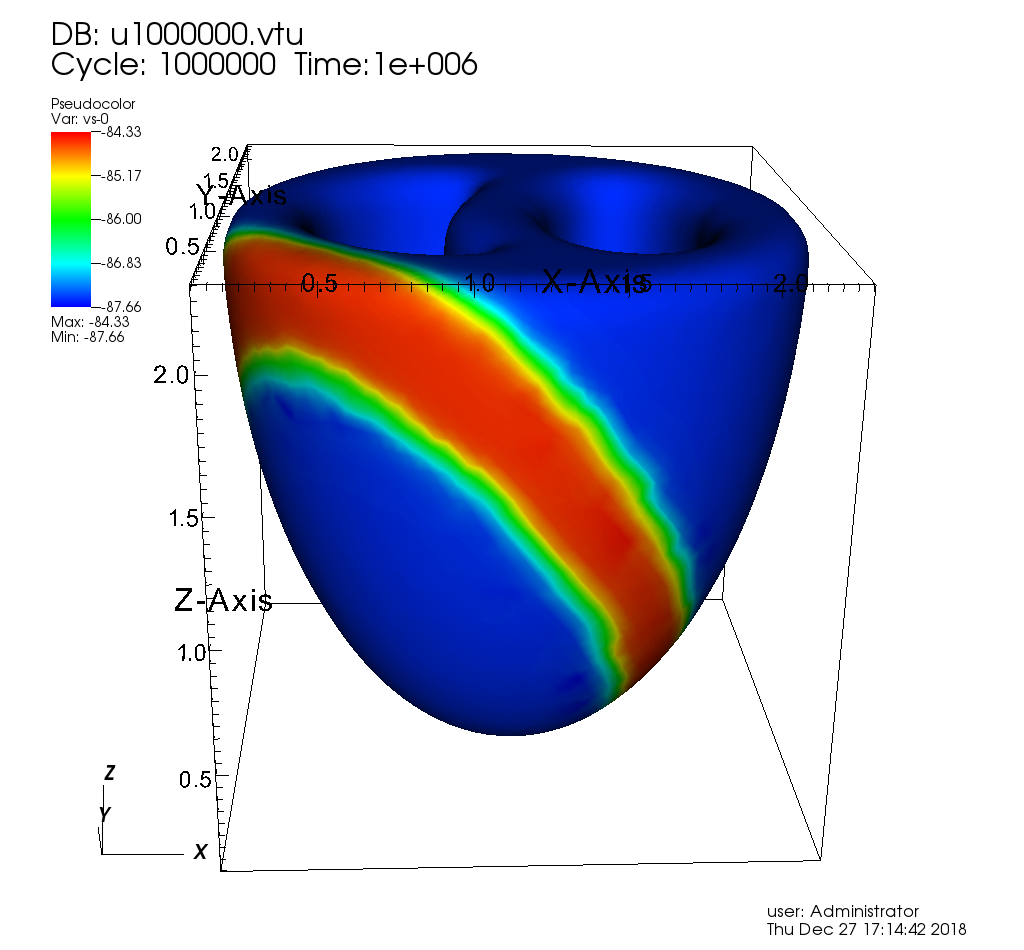
\includegraphics[width=0.3\textwidth,height=0.3\textwidth]{figures/visit0001.png}}}
	\hspace{0.2\textwidth}
	\subfigure[$t=3~ms$]{
		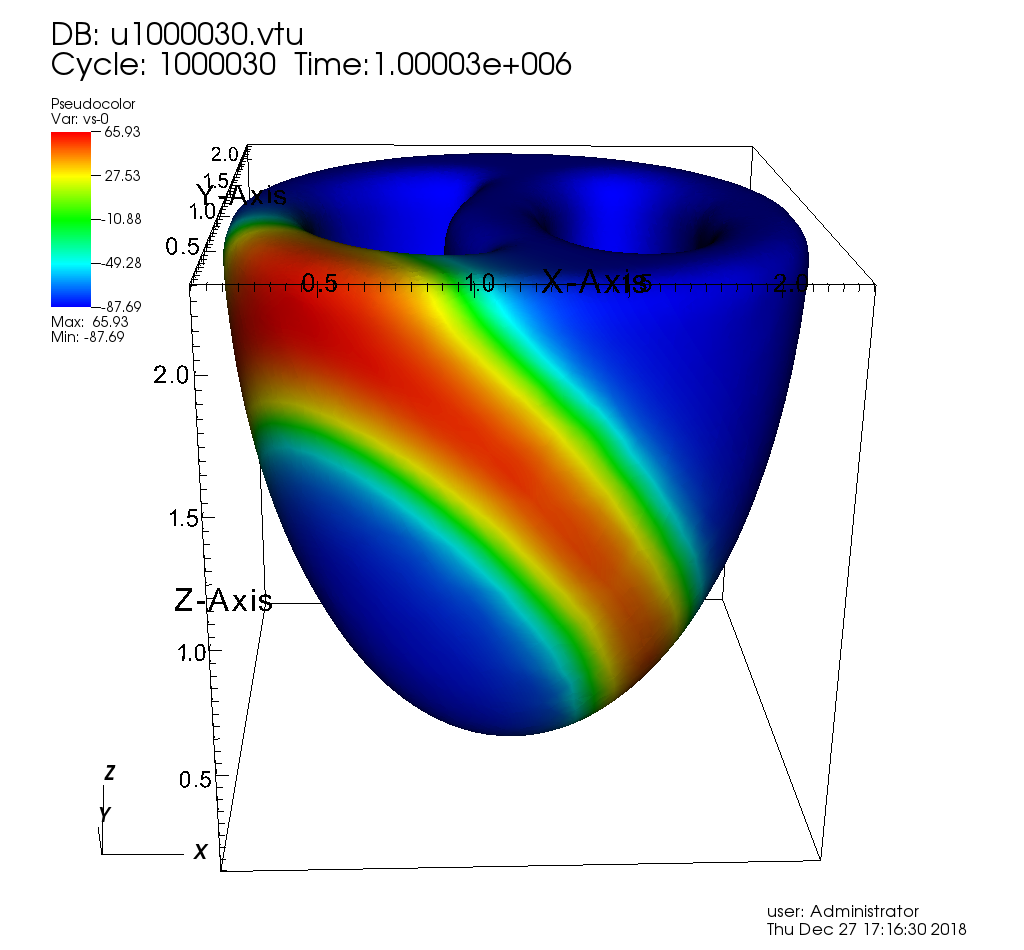
\includegraphics[width=0.3\textwidth,height=0.3\textwidth]{figures/visit0003.png}}
	\hspace{0.2\textwidth}
	\subfigure[$t=3.5~ms$]{
		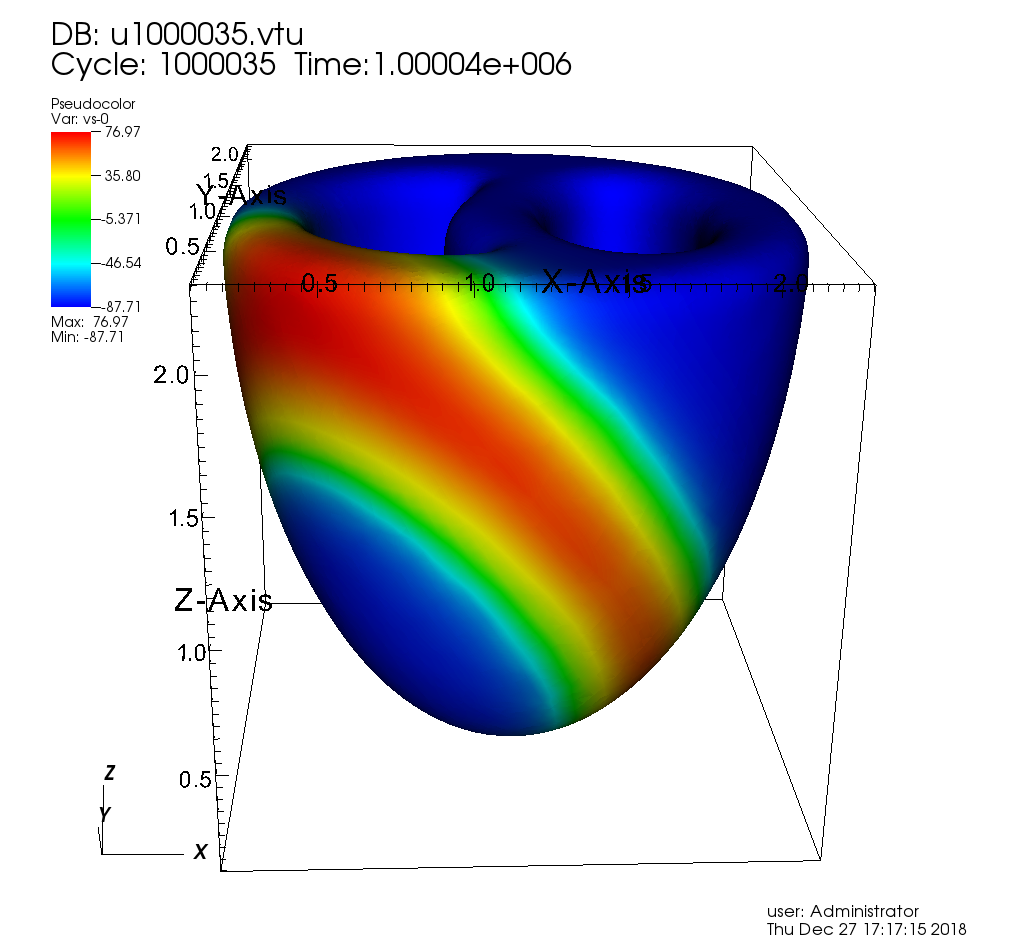
\includegraphics[width=0.3\textwidth,height=0.3\textwidth]{figures/visit0004.png}}
	\hspace{0.2\textwidth}
	\subfigure[$t=4~ms$]{
		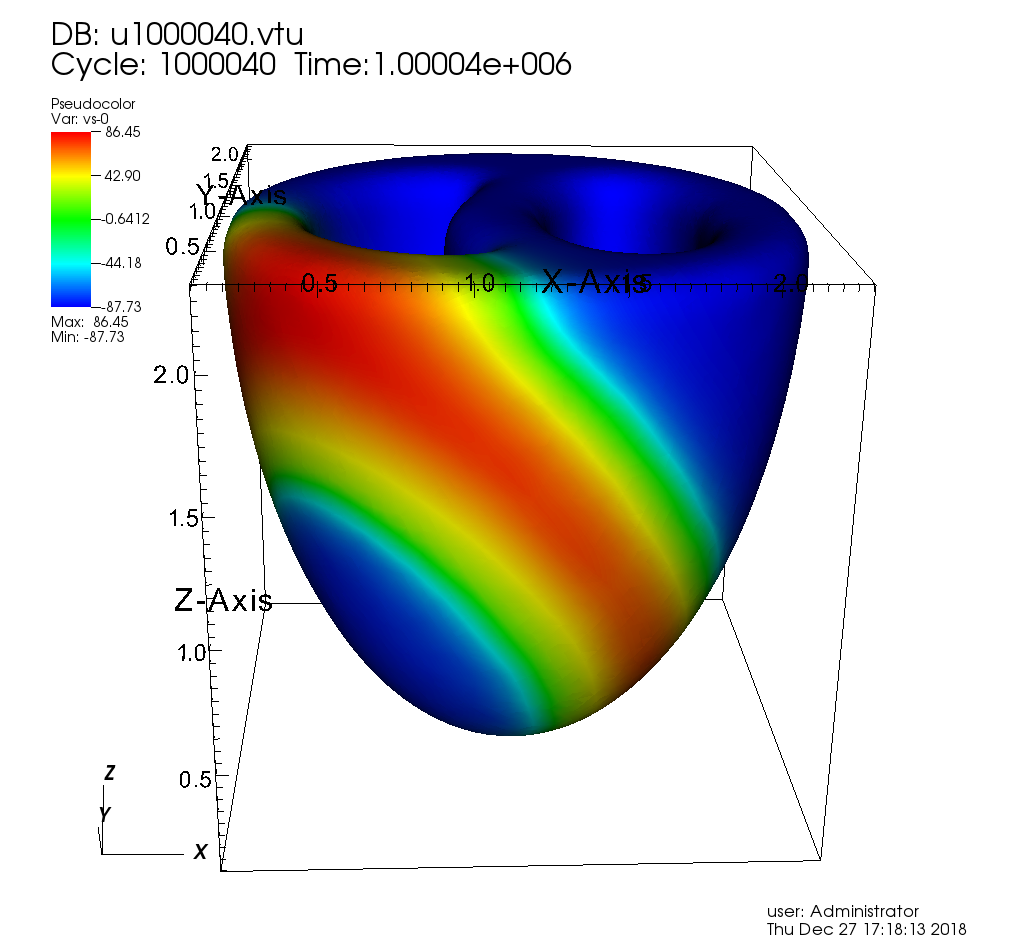
\includegraphics[width=0.3\textwidth,height=0.3\textwidth]{figures/visit0006.png}}
	\caption{三维ORd单域模型跨膜电势的传播轨迹}
	\label{fig6}
\end{figure}
\section{本章小结}
本章主要介绍了ORd单域模型的反应-扩散系统,总的离子流的构成形式,用有限元方法结合一阶算子分裂算法求解了基于三维左右心室结构的ORd单域模型,通过给定恰当的初边值条件,可以看到跨膜电势的传播轨迹,求解该模型,便于以后研究离子流的改变对跨膜电势传播状态的影响,为心律失常等疾病的预防和治疗提供研究基础。


%==============第六章节内容==================
\chapter{总结与展望}

\section{工作总结}
心律失常及心室颤动等心脏疾病已经成为导致人类死亡的常见疾病,而心律失常则是由于心脏电活动机制出现了紊乱,对心脏电活动的研究已经越来越受到人们的关注。借助计算机等技术,通过对心脏电活动进行数值仿真,在心脏疾病的治疗诊断方面发挥了强大的作用。
有限元方法有扎实的理论基础,对不规则几何形状的适应性较好,便于运用到3D心脏结构的数值模拟,并且最终可以归为代数方程组的求解问题,有广泛的应用前景。
本文主要用基于有限元方法开展了一下工作:
由双域模型简化而来的单域模型是一个非线性的反应-扩散系统,由一个偏微分方程和一个常微分方程耦合而成,首先对常用的时间离散格式进行了总结,本文针对非线性反应项,采用了显-隐时间离散格式,用有限元方法求解了二维FHN单域模型,并且证明了完全离散的显-隐有限元方法的稳定性和收敛性。当$\tau<\min\{\frac{2}{(1-a)^2+2+2\varepsilon^2\beta^2},\frac{1}{2(1-\varepsilon\gamma)}\}$~时,数值格式是稳定的;当$\tau<\min\{\frac{1}{8(4C_1(1+a)^2+a^2+4C_3)+2\varepsilon^2\beta^2},\frac{1}{2\varepsilon^2\gamma^2+4}\}$~时,$u$~基于~$H^1$~范数的收敛阶为$O(\tau+h)$;当~$\tau<\min\{\frac{1}{2(1+a+\varepsilon^2\beta^2+(1+a)C_u^1+(C_u^2)^2+2C_u^1C_u^2)},\frac{1}{2(2\varepsilon^2\gamma^2+2)}\}$~时,$u$~ 和~$v$~基于~$L^2$~范数的收敛阶为~$O(\tau+h^2)$。通过数值算例进行验证,收敛性结果与理论分析是一致的,并且运用适当的初边值条件,得到了稳定了螺旋波运动轨迹,也体现了完全离散的显-隐有限元方法的稳定性。利用有限元方法对几何空间适应性较好的特点,可以用来对三位心室或心脏进行数值模拟,将显-隐有限元方法扩展到三维人类左心室结构的FHN单域模型,通过适当的初边值条件,可以观察到跨膜电势的传播轨迹。

考虑到单域模型是一个耦合的反应-扩散系统,特别是膜模型包含多个离子流时,控制方程会很复杂。本文中还研究了算子分裂技术,可以将整个系统分成几个容易求解的子系统,为计算提供了方便。首先用一阶算子分裂有限元方法求解了二维FHN单域模型,数值算例的结果显示,也得到了稳定的螺旋波,并将该方法求解基于三维人工左右心室的FHN单域模型,得到了稳定的跨膜电势的传播状态,体现有限元方法结合算子分裂技术也是可行的。

ORd单域模型包含14种离子流,涉及近40个变量,是一个相对复杂的反应-扩散系统,进而用一阶算子分裂有限元方法求解了基于三维左右心室的ORd模型,得到了跨膜电势的传播轨迹,为以后求解更符合心脏电活动机制的复杂双域模型奠定了基础,有助于三维心脏电生理学更深层次的研究。
\section{工作展望}
现在基于心脏的电生理学模拟越来越引起人们的关注,这些模型能基本反映电生理学机制的同时,都在一定程度上进行了假设和简化。
本文主要利用有限元方法对描述心脏电活动的FHN单域模型和ORd单域模型进行了数值求解,通过数值算例验证了有限元方法的正确性。
在针对更接近心脏电活动机制的复杂模型以及提高数值模拟的效率和精度方面,还需要进一步的研究。

(1)模型选择。本文重点研究了双域域模型简化后的FHN双变量单域模型和ORd单域模型,不能更好的解释心脏电活动的行为状态。可以运用双域模型,其中的膜模型采用多个离子流,使仿真结果更能反映实际生理及病理状态。

(2)螺旋波动力学。本文中以简单的数值模拟,激发了再入波的形成,可以采用切波法或者交叉场法,来激发螺旋波的生成。当运用更复杂的膜模型时,可以针对离子流及电导率的取值大小,心脏组织出现局部缺血,梗塞等病态情况时,对螺旋波的稳定和失稳状态进行研究,为心律失常疾病的诊断与治疗提供依据。

(3)数值方法。本文中的数值模拟,都是采用固定的网格尺寸和时间步长,可以采用空间-时间自适应有限元方法为解决方案,提高数值仿真效率,探究螺旋波尖端更精细的传播行为。

(4)电力耦合。心脏是一个复杂的多尺度系统,心脏组织的电活动与心脏收缩和舒张状态等力学行为有很大的关系,对心脏电生理学及心脏组织中的力学行为耦合问题的研究已经成为一个重要的研究方向。

\backmatter
\bibliographystyle{nputhesis}
%\bibliography{ref}
\begin{thebibliography}{99}
	%\addcontentsline{toc}{chapter}{\protect\numberline{}{参考文献}}
	\addtolength{\itemsep}{-1.1em} % 缩小参考文献间的垂直间距
%	\markboth{参考文献}{参考文献}
	\bibitem{AHA2018}Benjamin E, Virani S, et al. Heart Disease and Stroke Statistics—2018 Update: A Report From the American Heart Association[J]. Circulation, 2018, 137(12):167-492.
	\bibitem{china2016}中国心血管病报告编写组. 《中国心血管病报告2016》概要[J]. 中国循环杂志, 2017, 32(6).
	\bibitem{broken1999}Entcheva E, Trayanov N A, Claydon F J. Patterns of and mechanisms for shock-induced polarization in the heart: a bidomain analysis[J]. IEEE Trans Biomed Eng, 1999, 46(3):260-270.
	\bibitem{broken1994}Roth B J. Mechanisms for electrical stimulation of excitable tissue.[J]. Crit Rev Biomed Eng, 1994, 22(22):253-305.
	\bibitem{china2004}张海澄. 正确评价抗心律失常药物的副作用[J]. 中国医师进修杂志, 2004, 27(1):3-6.
	\bibitem{dian2004}马慧. 心脏电复律并发症的观察及护理[J]. 职业与健康, 2004, 20(9):36-37.
	\bibitem{Bernus2002}Bernus O, Wilders R, Zemlin C W, et al. A computationally efficient electrophysiological model of human ventricular cells[J]. Am J Physiol Heart Circ Physiol, 2002, 282(6):H2296.
	\bibitem{Ten2006}Ten Tusscher K H, Bernus O, Hren R, et al. Comparison of electrophysiological models for human ventricular cells and tissues[J]. Progress in Biophysics \& Molecular Biology, 2006, 90(1-3):326.
	\bibitem{Nickerson2010}Nickerson D P, Hunter P J. Cardiac cellular electrophysiological modeling[J]. Cardiac Electrophysiology Methods \& Models, 2010:135-158.
	\bibitem{Shuaiby2013}Shuaiby S M, Hassan M A, Sharkawy A B, et al. A finite element model for the electrical activity in human cardiac tissues[J]. J. Eco. Heal. Env, 2013, 1: 25-33.
	\bibitem{Groenendaal2015}Groenendaal W, Ortega F A, Kherlopian A R, et al. Cell-specific cardiac electrophysiology models[J]. Plos Computational Biology, 2015, 11(4):e1004242.
	\bibitem{Sachse2004}Sachse F B. Computational cardiology[M]. Springer Berlin Heidelberg, 2004.
	\bibitem{Ying2005}Ying W. A multilevel adaptive approach for computational cardiology[M]. Duke University, 2005.
	\bibitem{HH1952yu}Hodgkin A L, Huxley A F. Propagation of electrical signals along giant nerve fibers[J]. Proceedings of the Royal Society of London, 1952, 140(899):177.
	\bibitem{HH1952}Hodgkin A L, Huxley A F. A quantitative description of membrane current and its application to conduction and excitation in nerve[J]. Bulletin of Mathematical Biology, 1952, 52(4):500–544.
	\bibitem{HH1952a}Hodgkin A L, Huxley A F. Currents carried by sodium and potassium ions through the membrane of the giant axon of Loligo[J]. Journal of Physiology, 1952, 116(4):449.
	\bibitem{HH1952b}Hodgkin A L, Huxley A F. The components of membrane conductance in the giant axon of Loligo[J]. Journal of Physiology, 1952, 116(4):473.
	\bibitem{FitzHugh1961}FitzHugh, Richard. Impulses and physiological states in theoretical models of nerve membrane[J]. Biophysical Journal, 1961, 1(6):445.
	\bibitem{Nagumo1962}Nagumo J, Arimoto S, Yoshizawa S. An active pulse transmission line simulating nerve axon[J]. Proceedings of the Ire, 1962, 50(10):2061-2070.
	\bibitem{Beer1977}Beeler G W, Reuter H. Reconstruction of the action potential of ventricular myocardial fibres[J]. Journal of Physiology, 1977, 268(1):177–210.
	\bibitem{Luo1991}Luo C H, Rudy Y. A model of the ventricular cardiac action potential. Depolarization, repolarization, and their interaction[J]. Circulation Research, 1991, 68(6):1501-1526.
	\bibitem{ORD2011}O'Hara T, Virág L, Varró A, et al. Simulation of the Undiseased Human Cardiac Ventricular ActionPotential: Model Formulation and Experimental Validation[J]. Plos Computational Biology, 2011, 7(5):e1002061.
	\bibitem{3D1}Zhang H, Ye H, Huang W. A Meshfree Method for Simulating Myocardial Electrical Activity[J]. Computational and Mathematical Methods in Medicine, 2012,(2012-9-3), 2012, 2012(3):936243.
	\bibitem{3D2}Belhamadia Y, Fortin A, Bourgault Y. Towards accurate numerical method for monodomain models using a realistic heart geometry[J]. Mathematical Biosciences, 2009, 220(2):89-101.
	\bibitem{3D3}Arevalo H, Rodriguez B, Trayanova N. Arrhythmogenesis in the heart: Multiscale modeling of the effects of defibrillation shocks and the role of electrophysiological heterogeneity[J]. Chaos, 2007, 17(1):25-290.
	\bibitem{bodo1983}Geselowitz D B , Rd M W . A bidomain model for anisotropic cardiac muscle[J]. Annals of Biomedical Engineering, 1983, 11(3-4):191-206.
	\bibitem{EJ1}Vigmond E J, dosSantos R W, Prassl A J, et al. Solvers for the cardiac Bidomain equations, Progress in Biophysics Molecular Biology. 2008, 96(1-3):3-18.
	\bibitem{JS1}Sundnes J, Lines G T, Cai X, et al. Computing the Electrical Activity in the Heart, Springer-Verlag, Berlin, 2006.
	\bibitem{Cla2011}Clayton R H, Bernus O, Cherry E M, et al. Models of cardiac tissue electrophysiology: progress, challenges and open questions[J]. Progress in Biophysics \& Molecular Biology, 2011, 104(1):22-48.
	\bibitem{Per1993}Pertsov A M, Davidenko J M, Salomonsz R, et al. Spiral waves of excitation underlie reentrant activity in isolated cardiac muscle[J]. Circulation Research, 1993, 72(3):631.
	%\bibitem{GGL}Gerardo-Giorda, Luca. (2008). Modeling and numerical simulation of action potential patterns in human atrial tissues.
	\bibitem{ND1}Noble D. Modelling the heart: insights, failures and progress[J]. Bioessays News \& Reviews in Molecular Cellular \& Developmental Biology, 2002, 24(12):1155.
	\bibitem{Vig2008}Vigmond E J, Weber dos Santos R, Prassl A J, et al. Solvers for the cardiac bidomain equations[J]. Progress in Biophysics and Molecular Biology, 2008, 96(1):3-18.
	\bibitem{sprial2006}Lopshire, J C. Sudden Cardiac Death: Better Understanding of Risks, Mechanisms, and Treatment[J]. Circulation, 2006, 114(11):1134-1136.
	\bibitem{Clayton2008}Clayton R H, Panfilov A V. A guide to modelling cardiac electrical activity in anatomically detailed ventricles[J]. Progress in Biophysics and Molecular Biology, 2008, 96(1-3):19-43.
	
	\bibitem{ouyang2001}欧阳颀. 反应扩散系统中螺旋波的失稳[J]. 物理, 2001, 30(1):30-36.
	\bibitem{tangguoning2010}钟敏, 唐国宁. 用钙离子通道激动剂抑制心脏组织中的螺旋波和时空混沌[J]. 物理学报, 2010, 59(5):3070-3076.
	\bibitem{yuan2005}袁国勇, 杨世平, 王光瑞, et al. 两个延迟耦合FitzHugh-Nagumo系统的动力学行为[J]. 物理学报, 2005, 54(4):1510-1522.
	\bibitem{gao2011}高加振, 谢玲玲, 谢伟苗, et al. FitzHugh-Nagumo系统中螺旋波的控制[J]. 物理学报, 2011, 60(8):59-67.
	
	\bibitem{Buweiping2015}Bu W, Tang Y, Wu Y, et al. Crank-Nicolson ADI Galerkin finite element method for two-dimensional fractional FitzHugh-Nagumo monodomain model[J]. Applied Mathematics \& Computation, 2015, 257(C):355-364.
	\bibitem{LFW2015}Liu F, Zhuang P, Turner I, et al. A semi-alternating direction method for a 2-D fractional FitzHugh–Nagumo monodomain model on an approximate irregular domain[J]. Journal of Computational Physics, 2015, 293(C):252-263.
	\bibitem{LFW2012}Liu F, Turner I, Anh V, et al. A numerical method for the fractional Fitzhugh-Nagumo monodomain model[J]. Anziam Journal, 2012, 54:C608-C629.
	\bibitem{YZZ2017}Yang Z, Yuan Z, Nie Y, et al. Finite element method for nonlinear Riesz space fractional
	diffusion equations on irregular domains[J]. Journal of Computational Physics, 2017, 330:863-883.
	\bibitem{Pertsov1993}Pertsov A V. Spiral waves of excitation underlie reentrant activity in isolated cardiac muscle[J]. Circulation Research, 1993, 72(3):631.
	\bibitem{chafen2000}Cherry E M, Greenside H S, Henriquez C S. A Space-Time Adaptive Method for Simulating Complex Cardiac Dynamics[J]. Physical Review Letters, 2000, 84(6):1343-1346.
	\bibitem{SM1}Shuaiby S M, Hassan M A, ElMelegy M, Modeling and Simulation of The Action Potential In Human Cardiac Tissues Using Finite Element Method[J], Archives of Physical Medicine \& Rehabilitation, 2012, 2(3):21-27.
	\bibitem{GG2008}Gerardo-Giorda L. Modeling and numerical simulation of action potential patterns in human atrial tissues[J]. Giorda, 2008.
	
	\bibitem{Vincent2015}Vincent K P, Gonzales M J, Gillette A K, et al. High-order finite element methods for cardiac monodomain simulations[J]. Frontiers in Physiology, 2015, 6:217.
	\bibitem{Dickopf2014}Dickopf T, Krause D, Krause R, et al. Design and analysis of a lightweight parallel adaptive scheme for the solution of the monodomain equation[J]. Siam Journal Onentific Computing, 2014, 36(2).
	\bibitem{Trangenstein2000}Trangenstein J A, Skouibine K and Allard W K, Operator splitting and mesh refinement for the ftzhugh-nagumo problem, 2000.
	\bibitem{Belhamadia2009}Belhamadia Y, Fortin A, Bourgault Y. Towards accurate numerical method for monodomain models using realistic heart geometry[J]. Mathematical Biosciences, 2009, 220(2):89.
	\bibitem{Bendahmane2010}Bendahmane M , Raimund Bürger, Ruiz-Baier R. A finite volume scheme for cardiac propagation in media with isotropic conductivities[J]. Mathematics and Computers in Simulation, 2010, 80(9):1821-1840.
	\bibitem{zhang2005}Zhang H and Shi P, A meshfree method for solving cardiac electrical propagation[C], International Conference of the Engineering in Medicine \& Biology Society, 2005 IEEE Engineering in Medicine and Biology 27th Annual Conference, 2005, 1(1):349-352.
	\bibitem{Jackson1990}Jackson D E, Existence and regularity for the Fitzhugh-Nagumo equations with inhomogeneous
	boundary conditions[J], Nonlinear Analysis, 1990, 14(3):201-216.
	\bibitem{Jackson1992}Jackson D E, Error estimates for the semidiscrete Galerkin approximations of the Fitzhugh-Nagumo equations[J], Applied Mathematics and Computation, 1992, 50(1):93-114.
	\bibitem{Jerome1980}Jerome J W, Convergence of successive iterative semidiscretizations for Fitzhugh-Nagumo reac-
	tion diffusion systems[J], SIAM Journal on Numerical Analysis, 1980, 17(2):192-206.
	\bibitem{SAN1996}Sanfelici S, Numerical and analytic study of a parabolic-ordinary system modelling cardiac activation under equal anisotropy conditions[J], Rivista Di Matematica Della Universita Di Parma, 1996, 5(5):143-157.
	\bibitem{ovvr2015}Elshrif M M, Shi P, Cherry E M. Representing Variability and Transmural Differences in a Model of Human Heart Failure[J]. IEEE Journal of Biomedical \& Health Informatics, 2015, 19(4):1308-1320.
	\bibitem{ovvr2013}Christophe, Bernard. Simulation of early after-depolarisation in non-failing human ventricular myocytes: Can this help cardiac safety pharmacology?[J]. Pharmacological Reports, 2013, 65(5):1281-1293.
	
	\bibitem{ord1}Chen M H, Chen P Y , Luo C H. Quadratic adaptive algorithm for solving cardiac action potential models[J]. Computers in Biology and Medicine, 2016, 77: 261-273.
	\bibitem{ovvr2017}Whittaker D G, Haibo N, Benson A P , et al. Computational Analysis of the Mode of Action of Disopyramide and Quinidine on hERG-Linked Short QT Syndrome in Human Ventricles[J]. Frontiers in Physiology, 2017, 8:759-.
	\bibitem{ovvr2012}Trenor B, Gomis-Tena J , Ferrero J M , et al. A simulation tool to assess the pro-arrhythmic potential of ion channel blockers[C]. Computing in Cardiology. IEEE, 2012.
	\bibitem{ovvr20141}Elshrif M M , Shi P , Cherry E M . Electrophysiological properties under heart failure conditions in a human ventricular cell: A modeling study[J]. Conf Proc IEEE Eng Med Biol Soc, 2014, 2014:4324-4329.
	\bibitem{ovvr20142}Elshrif M M , Cherry E M . A Quantitative Comparison of the Behavior of Human Ventricular Cardiac Electrophysiology Models in Tissue[J]. PLOS ONE, 2014, 9.
	\bibitem{ovvr20172}Dutta S, Mincholé, Ana, Quinn T A , et al. Electrophysiological properties of computational human ventricular cell action potential models under acute ischemic conditions[J]. Progress in Biophysics and Molecular Biology, 2017:S0079610716300918.
	\bibitem{2d2003}Bourgault Y, Ethier M, Leblanc V G. Simulation of Electrophysiological Waves with an Unstructured Finite Element Method[J]. Esaim Proceedings, 2003, 37(4):649-661.
	\bibitem{3d2007}Arevalo H, Rodriguez B , Trayanova N . Arrhythmogenesis in the heart: Multiscale modeling of the effects of defibrillation shocks and the role of electrophysiological heterogeneity[J]. Chaos, 2007, 17(1):25-290.
	\bibitem{3d2009}Deuflhard P, Erdmann B , Roitzsch R , et al. Adaptive finite element simulation of ventricular fibrillation dynamics[J]. Computing \& Visualization in Science, 2009, 12(5):201-205.
	\bibitem{3d2005}Rodriguez, B. Differences Between Left and Right Ventricular Chamber Geometry Affect Cardiac Vulnerability to Electric Shocks[J]. Circulation Research, 2005, 97(2):168-175.
	\bibitem{3d20009}Prassl A J, Kickinger F, Ahammer H, et al. Automatically Generated, Anatomically Accurate Meshes for Cardiac Electrophysiology Problems[J]. IEEE transactions on bio-medical engineering, 2009, 56(5):1318-30.
	
	
	\bibitem{FEM2010}陈锡栋, 杨婕, 赵晓栋等. 有限元法的发展现状及应用[J]. 机械设计与制造工程, 2010, 39(11):6-8.
	\bibitem{begin1986}章本照. 流体力学中的有限元方法[M]. 机械工业出版社, 1986.
	
	\bibitem{Courant1943}Courant R. Variational methods for the solution of problems of equilibrium and vibrations[J]. Bulletin of the American Mathematical Society, 1943, 49(1943):1-23.
	\bibitem{Turner1956}Turner M J, Clough R W, Martin H C, et al. Stiffness and Deflection Analysis of Complex Structures[J]. J.aero.sci, 1956, 23(9):805-823.
	\bibitem{Clough1960}Clough R W. The Finite Element Method in Plane Stress Analysis. proceeding of the second ASEC Conference on Electronic Computation Pittsburgh, PA, 1960, 9(3):345-347.
	\bibitem{Hu1954}胡海昌.论弹性体力学和受范性体力学中的一般变分原理.物理学报,1954,10(3):259—289.
	\bibitem{Feng1965}冯康. 基于变分原理的差分格式[J]. 应用数学与计算数学, 1965, 2(4):238―262.
	\bibitem{shi2000}石钟慈, 王家城. 一类非协调元的收敛性分析[J]. 计算数学, 2000, 22(1):97-2.
	\bibitem{Feng2001}Feng X , Karakashian O A . Two-Level Additive Schwarz Methods for a Discontinuous Galerkin Approximation of Second Order Elliptic Problems[J]. SIAM Journal on Numerical Analysis, 2001, 39(4):1343-1365.
	\bibitem{ANSYS2000}蓝宇, 张连杰. 大型有限元分析软件ANSYS[J]. 应用科技, 2000, 27(6):11-12.
	\bibitem{L2003}Logan著 D L. 有限元方法基础教程[J]. 2003.
	\bibitem{fanhan2006}刘培德. 泛函分析基础[M]. 科学出版社, 2006.
	\bibitem{holder2013}乔建斌. $H\ddot{o}lder$不等式的离散形式与积分形式的推广[J]. 河南科学, 2013(2):127-129.
	\bibitem{Shi2010}石钟慈, 王鸣. 有限元方法[M]. 科学出版社, 2010.
	\bibitem{Chen2010}Chen, Wu Z , Haijun. Selected topics in finite element methods =[M]. Science Press, 2010.
	\bibitem{qianru2012}杜其奎, 陈金如. 有限元方法的数学理论[M]. 科学出版社, 2012.
	\bibitem{ouyang2000}欧阳颀. 反应扩散系统中的斑图动力学[M]. 上海科技教育出版社, 2000.
	\bibitem{exist1978}Rauch J, Smoller J. Qualitative theory of the FitzHugh-Nagumo equations[J]. Advances in Mathematics, 1978, 27(1):12-44.
	\bibitem{bianzhi1978}Schonbek M E. Boundary value problems for the Fitzhugh-Nagumo equations[J]. Journal of Differential Equations, 1978, 30(1):119-147.
	\bibitem{He2003}He Y, A fully discrete stabilized finite-element method for the time-dependent Navier-Stokes prob-
	lem. Ima Journal of Numerical Analysis, 2003, 23(4):665-691.
	\bibitem{Caili2015}Cai L, Gao H, Luo X, et al. Multi-scale modelling of the human left ventricle[J]. Scientia Sinica Physica Mechanica \& Astronomica, 2015, 45(2):024702.
	\bibitem{b1994}Brener S C and Scott L R, The Mathematical Theory of Finite Element Methods, Springer-Verlag, New York, 1994.
	\bibitem{CiarletPG}Ciarlet P G, The Finite Element Method for Elliptic Problems, North-Holland, Amsterdam, 1978.
	
	\bibitem{split2006}Sundnes J, Lines G T, Cai X, et al. Computing the Electrical Activity in the Heart[J]. 2006.
	\bibitem{split2008}Vigmond E J, Santos R W D, Prassl A J, et al. Solvers for the Cardiac Bidomain Equations[J]. Progress in Biophysics \& Molecular Biology, 2008, 96(1):3-18.
	\bibitem{split2007}Schroll H J, Lines G T, Tveito A. On the accuracy of operator splitting for the monodomain model of electrophysiology[J]. International Journal of Computer Mathematics, 2007, 84(6):871-885.
	\bibitem{bodo2009}Linge S, Sundnes J, Hanslien M, et al. Numerical solution of the bidomain equations[J]. Philosophical Transactions of the Royal Society A: Mathematical, Physical and Engineering Sciences, 2009, 367(1895):1931-1950.
	\bibitem{fw2012}Liu F, Turner I, Anh V, et al, A numerical method for the fractional Fitzhugh-Nagumo monodomain model[J], Anziam Journal, 2012, 54:608-629.
	
	
	\bibitem{RL1978}Rush S, Larsen H. A practical algorithm for solving dynamic membrane equations[J]. IEEE Trans Biomed Eng, 1978, BME-25(4): 389-392.
	\bibitem{RL1985}Victorri B, Vinet A, Roberge F A, et al. Numerical integration in the reconstruction of cardiac action potentials using Hodgkin-Huxley-type models[J]. Computers \& Biomedical Research An International Journal, 1985, 18(1):10-23.
	

\end{thebibliography}
 
%\Appendix
%This is appendix.

\Thanks

时光荏苒,带走了青春,留下了回忆。随着毕业设计接近尾声,我在西北工业大学的学习生活即将告一段落。在这两年多的学习生活中,我掌握了许多学习技巧,养成了良好的学习习惯,提高了解决问题的能力,结识了善良可爱的朋友,培养了积极乐观的心态,收获颇丰。这些收获离不开我的指导老师,任课老师,师兄师姐,师弟师妹的帮助与关怀,在此对他们表示衷心的感谢,希望他们身体健康,工作顺利。

此次撰写毕业论文期间,获得了蔡力副教授的悉心指导。蔡老师在论文选题中,为我指引了方向,在研究过程中发现问题时,耐心的给我提供建议,在论文撰写时,对论文大方向和小细节把握透彻,多次为我提供建设性意见,使我的论文内容更丰富饱满。在学习阶段,蔡老师多次组织专家学者进行学术报告,提供了与专家教授之间学习交流的机会,不定期的组内汇报,督促我按时完成科研工作,并能及时解决遇到的问题,养成良好的学习习惯。除了学习科研方面,蔡老师还教会了我积极乐观,严于律己的生活态度。这些收获将是我宝贵的财富,在以后的工作中也会继续鼓励我,再次对蔡老师表示诚挚的感谢。在这里,我还要感谢荆菲菲老师,在我遇到问题时,能够耐心的给我解答,为我指出论文撰写中的细节错误,帮助我培养严谨务实的学习态度,他们都是我学习的榜样。

其次要感谢我204教研室的小伙伴们,在我的学习生活中,给予我帮助和关心。特别要感谢博士王永恒师兄,数值模拟阶段,在编程计算上给予我耐心的指导,为我解决问题,助我进步。感谢杨宗泽师兄,在理论分析上为我耐心解释,指点迷津。感谢我的同门及师弟师妹的帮助与关怀,希望他们在以后各自领域继续努力,取得更高的成就。

最后要感谢我的父母,他们是我学习生活中最坚实的后盾,给予我无微不至的关怀和爱。感谢645可爱的舍友,让我感受到在学校中“家”的温暖与快乐。感谢这些善良可爱的人,让我在西北工业大学的生活充满乐趣,陪伴我顺利完成硕士研究生学业。


\Work
% TODO 如何直接引用使参考文献的内容显示在这里
\begin{itemize}
\item[1] Cai L, Sun Y, Jing F, et al. A Fully Discrete Implicit-Explicit Finite Element Method for Solving the FitzHugh-Nagumo Model[J]. Journal of Computational Mathematics, 2017. (已投稿)
\item[2] 国家自然科学基金面上项目(11871399),受损心脏电力耦合问题高效数值模拟方法及其应用研究(2019.01-2022.12),负责人:蔡力
\item[3] 国家自然科学基金面上项目(11471261),人类左心室3D重构及相关流固耦合问题的数值方法研究(2015.01-2018.12),负责人:蔡力
\item[4] 陕西省自然科学基础研究计划面上项目(2017JM1005),左心室流固耦合系统的建模与数值计算(2017.01-2018.12),负责人:蔡力
\end{itemize}

\statement
\end{document}
